% =====================================================================
% User Guide (appendix guide) --- GENERATED from USER_GUIDE.md
% Regenerate with scratchpad build-appendix-guide.py; do not hand-edit.
% Screenshots live in Backmatter/UserGuideImages/ and are included via \IfFileExists,
% so a missing image shows a "screenshot pending" box until the PNG is added.
% Figures float ([htbp]) but are flushed per section (\FloatBarrier); they are
% kept out of the global List of Figures.
% Helper macros below are the minimal set the pandoc body relies on (\real comes
% from the calc package, already loaded by the thesis). They are guarded so two
% guides can be \input in the same document without clashing.
% =====================================================================
\providecommand{\tightlist}{\setlength{\itemsep}{0pt}\setlength{\parskip}{0pt}}
\makeatletter\@ifundefined{c@none}{\newcounter{none}}{}\makeatother % unnumbered tables
\providecommand{\guidescreenshotpending}[1]{\fbox{\parbox[c][3cm][c]{0.9\linewidth}{\centering\itshape Screenshot pending: place the image file at \texttt{#1}.}}}
\captionsetup{list=no}

\chapter{User Guide}\label{app:user-guide}

A handbook for researchers operating the Reading the Reader adaptive reading platform.

\FloatBarrier
\section{Overview}\label{1-overview}

Reading the Reader is a \textbf{researcher-operated} adaptive reading system. It connects to a
Tobii eye tracker, runs a controlled reading session for an invited participant, mirrors the
participant's screen for the researcher in real time, and can apply context-aware
micro-interventions while the participant reads. After a session, all data can be exported or
replayed for analysis.

A typical experiment moves through these stages:

\begin{enumerate}
\def\labelenumi{\arabic{enumi}.}
\tightlist
\item
  \textbf{Prepare content} --- save one or more reading texts as reusable \emph{reading materials}.
\item
  \textbf{Compose a template} --- combine materials into a reusable \emph{experiment template} with
  presentation defaults and a runtime strategy.
\item
  \textbf{Run a session} --- follow the guided stepper to set up the tracker, baseline, participant
  details, and calibration, then start reading.
\item
  \textbf{Monitor live} --- watch the participant's gaze, attention, and struggle signals; trigger or
  approve interventions.
\item
  \textbf{Export / replay} --- save the recorded session and review it later.
\end{enumerate}

\FloatBarrier
\section{Before You Start}\label{2-before-you-start}

{\small\def\LTcaptype{none} % do not increment counter
\begin{longtable}[]{@{}
  >{\raggedright\arraybackslash}p{(\linewidth - 2\tabcolsep) * \real{0.2500}}
  >{\raggedright\arraybackslash}p{(\linewidth - 2\tabcolsep) * \real{0.7500}}@{}}
\toprule\noalign{}
\begin{minipage}[b]{\linewidth}\raggedright
Requirement
\end{minipage} & \begin{minipage}[b]{\linewidth}\raggedright
Detail
\end{minipage} \\
\midrule\noalign{}
\endhead
\bottomrule\noalign{}
\endlastfoot
\textbf{Browser} & A Chromium-based browser is recommended. Fullscreen permission is required for calibration and the live view. \\
\textbf{Eye tracker} & A Tobii device connected to the Windows machine (for real eye-tracking sessions). \\
\textbf{Backend running} & The backend service must be running and reachable by the frontend. \\
\textbf{Two screens (recommended)} & One screen for the \textbf{Participant View}, one for the \textbf{Researcher Live View}. \\
\textbf{Content format} & Reading materials are \textbf{Markdown only}. PDF is not supported. \\
\end{longtable}
}

\begin{quote}
\textbf{Tip:} If you do not have hardware available, switch to \textbf{Mouse mode} in Settings to run a
demo where the participant's mouse position acts as synthetic gaze. See
\hyperref[7-sensing-modes-explained]{Sensing Modes}.
\end{quote}

\FloatBarrier
\section{Tour of the Workspace}\label{3-tour-of-the-workspace}

The workspace is where the researcher prepares, runs, and reviews experiments. The left
\textbf{sidebar} is the primary navigation the researcher uses to move between the reading-material
library, experiment templates, the live session view, replay, and settings. Each sidebar item is
described below.

{\small\def\LTcaptype{none} % do not increment counter
\begin{longtable}[]{@{}
  >{\raggedright\arraybackslash}p{(\linewidth - 2\tabcolsep) * \real{0.2500}}
  >{\raggedright\arraybackslash}p{(\linewidth - 2\tabcolsep) * \real{0.7500}}@{}}
\toprule\noalign{}
\begin{minipage}[b]{\linewidth}\raggedright
Sidebar item
\end{minipage} & \begin{minipage}[b]{\linewidth}\raggedright
What it's for
\end{minipage} \\
\midrule\noalign{}
\endhead
\bottomrule\noalign{}
\endlastfoot
\textbf{Home} & The researcher dashboard. Lists ``Ready to run'' templates and drafts; start or edit a template from here. \\
\textbf{Material Library} & Create, edit, export, and delete reusable reading materials. \\
\textbf{Experiment Templates} & Manage reusable experiment setups (ready / drafts / archived). Duplicate, export, edit, delete. \\
\textbf{Researcher Live} & The live monitoring view of the currently running session. \\
\textbf{Participant View} & Opens the participant-facing flow (opens in a new tab --- put this on the participant's screen). \\
\textbf{Replay} & Load a saved or exported session and play it back frame by frame. \\
\textbf{Settings} & Input mode, calibration point count, and reading-view (ReaderShell) defaults. \\
\end{longtable}
}

\begin{figure}[htbp]
\centering
\IfFileExists{Backmatter/UserGuideImages/Sidebar.png}{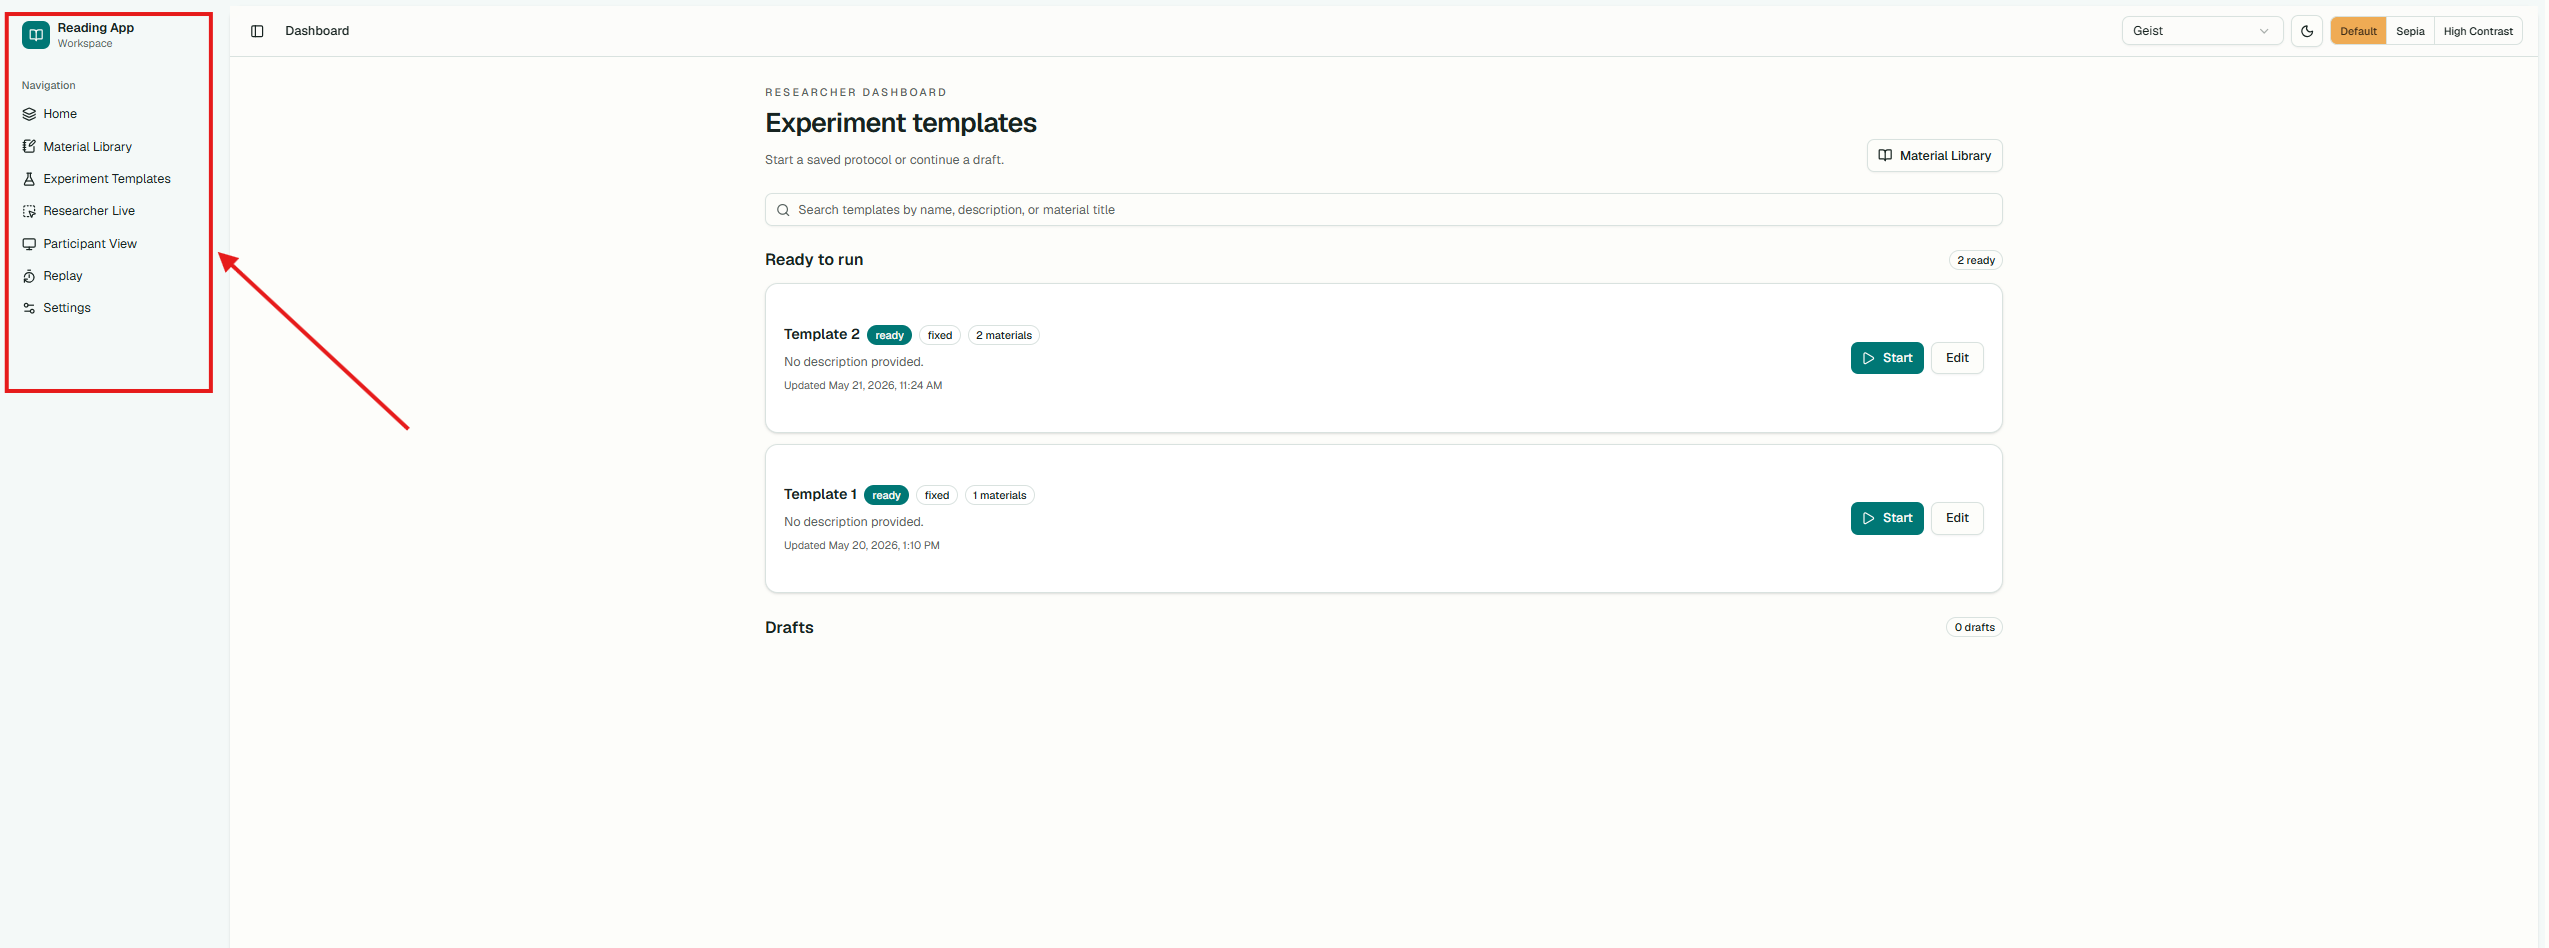
\includegraphics[width=\linewidth,height=0.86\textheight,keepaspectratio]{Backmatter/UserGuideImages/Sidebar.png}}{\guidescreenshotpending{Backmatter/UserGuideImages/Sidebar.png}}
\caption{The left sidebar, with every navigation item.}
\end{figure}

The \textbf{top bar} (right side) holds the app font selector, light/dark mode toggle, and color
palette toggle. These affect the app appearance.

\begin{figure}[htbp]
\centering
\IfFileExists{Backmatter/UserGuideImages/topbar.png}{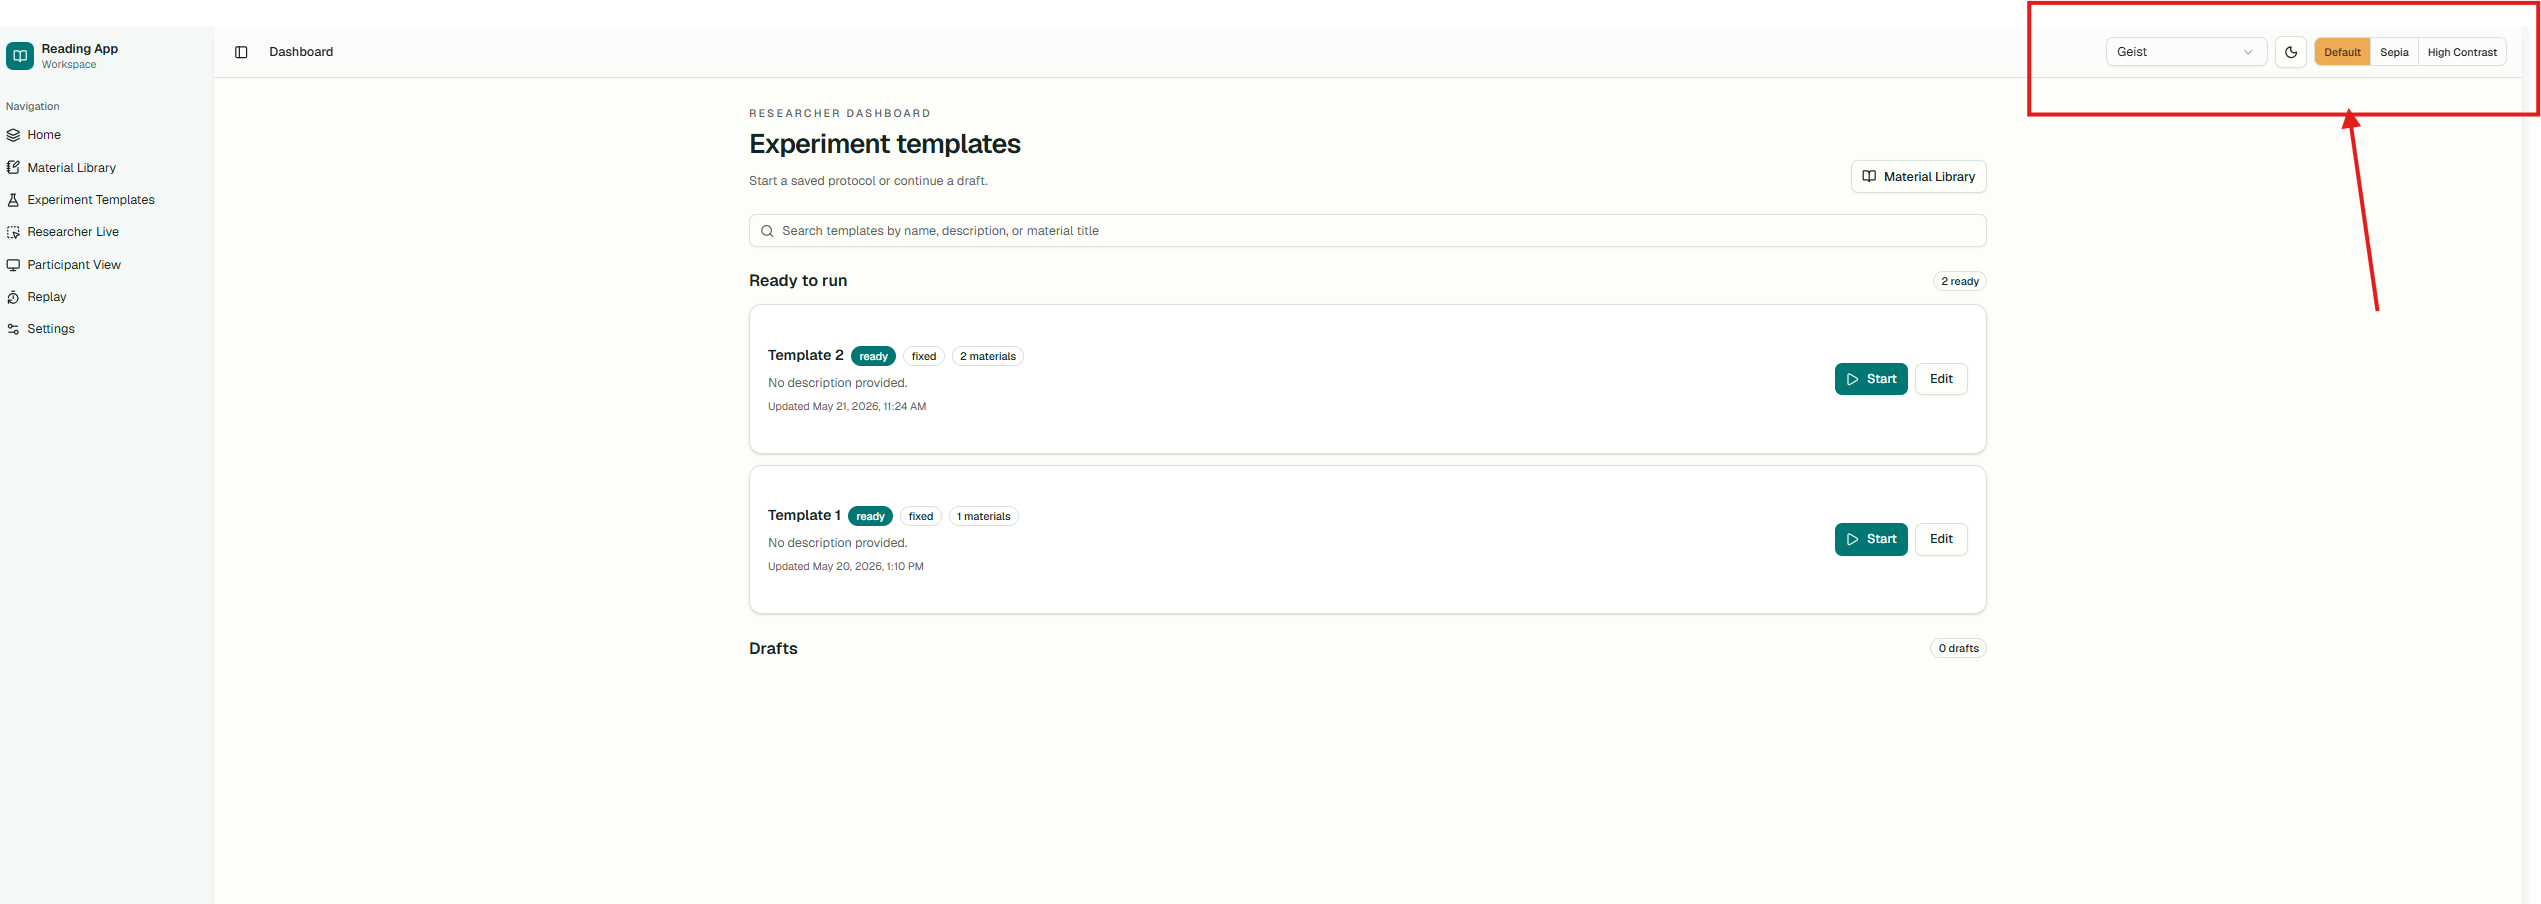
\includegraphics[width=\linewidth,height=0.86\textheight,keepaspectratio]{Backmatter/UserGuideImages/topbar.png}}{\guidescreenshotpending{Backmatter/UserGuideImages/topbar.png}}
\caption{The top bar controls (right side): app font selector, light/dark mode toggle, and color palette.}
\end{figure}

\FloatBarrier
\section{Quick Start (5-minute run)}\label{4-quick-start-5-minute-run}

If you just want to get a session going, follow this condensed path. Each step links to its full
section below.

\begin{enumerate}
\def\labelenumi{\arabic{enumi}.}
\tightlist
\item
  \textbf{Create at least one reading material} → \cref{51-create-a-reading-material}
\item
  \textbf{Build a template} from that material and mark it \textbf{Ready} → \cref{52-build-an-experiment-template}
\item
  From \textbf{Home}, click \textbf{Start} on the ready template → \cref{53-run-an-experiment-session}
\item
  Open the \textbf{Participant View} on the participant's screen → \cref{54-the-participant-view}
\item
  Complete \textbf{Step 1--4} of the stepper (tracker → baseline → participant info → calibration)
\item
  Click \textbf{Start reading session}, then open \textbf{Researcher Live} to monitor → \cref{56-the-live-researcher-view}
\item
  When done, \textbf{Finish experiment} and \textbf{export} the data → \cref{57-finishing--exporting-a-session}
\end{enumerate}

\FloatBarrier
\section{Step-by-Step Workflows}\label{5-step-by-step-workflows}

\subsection{Create a Reading Material}\label{51-create-a-reading-material}

A \emph{reading material} is one Markdown text plus its comprehension quiz and presentation defaults,
saved as a reusable baseline.

\begin{enumerate}
\def\labelenumi{\arabic{enumi}.}
\item
  In the sidebar, open \textbf{Material Library}.

\begin{figure}[htbp]
  \centering
\IfFileExists{Backmatter/UserGuideImages/OpenMaterialLibrary.png}{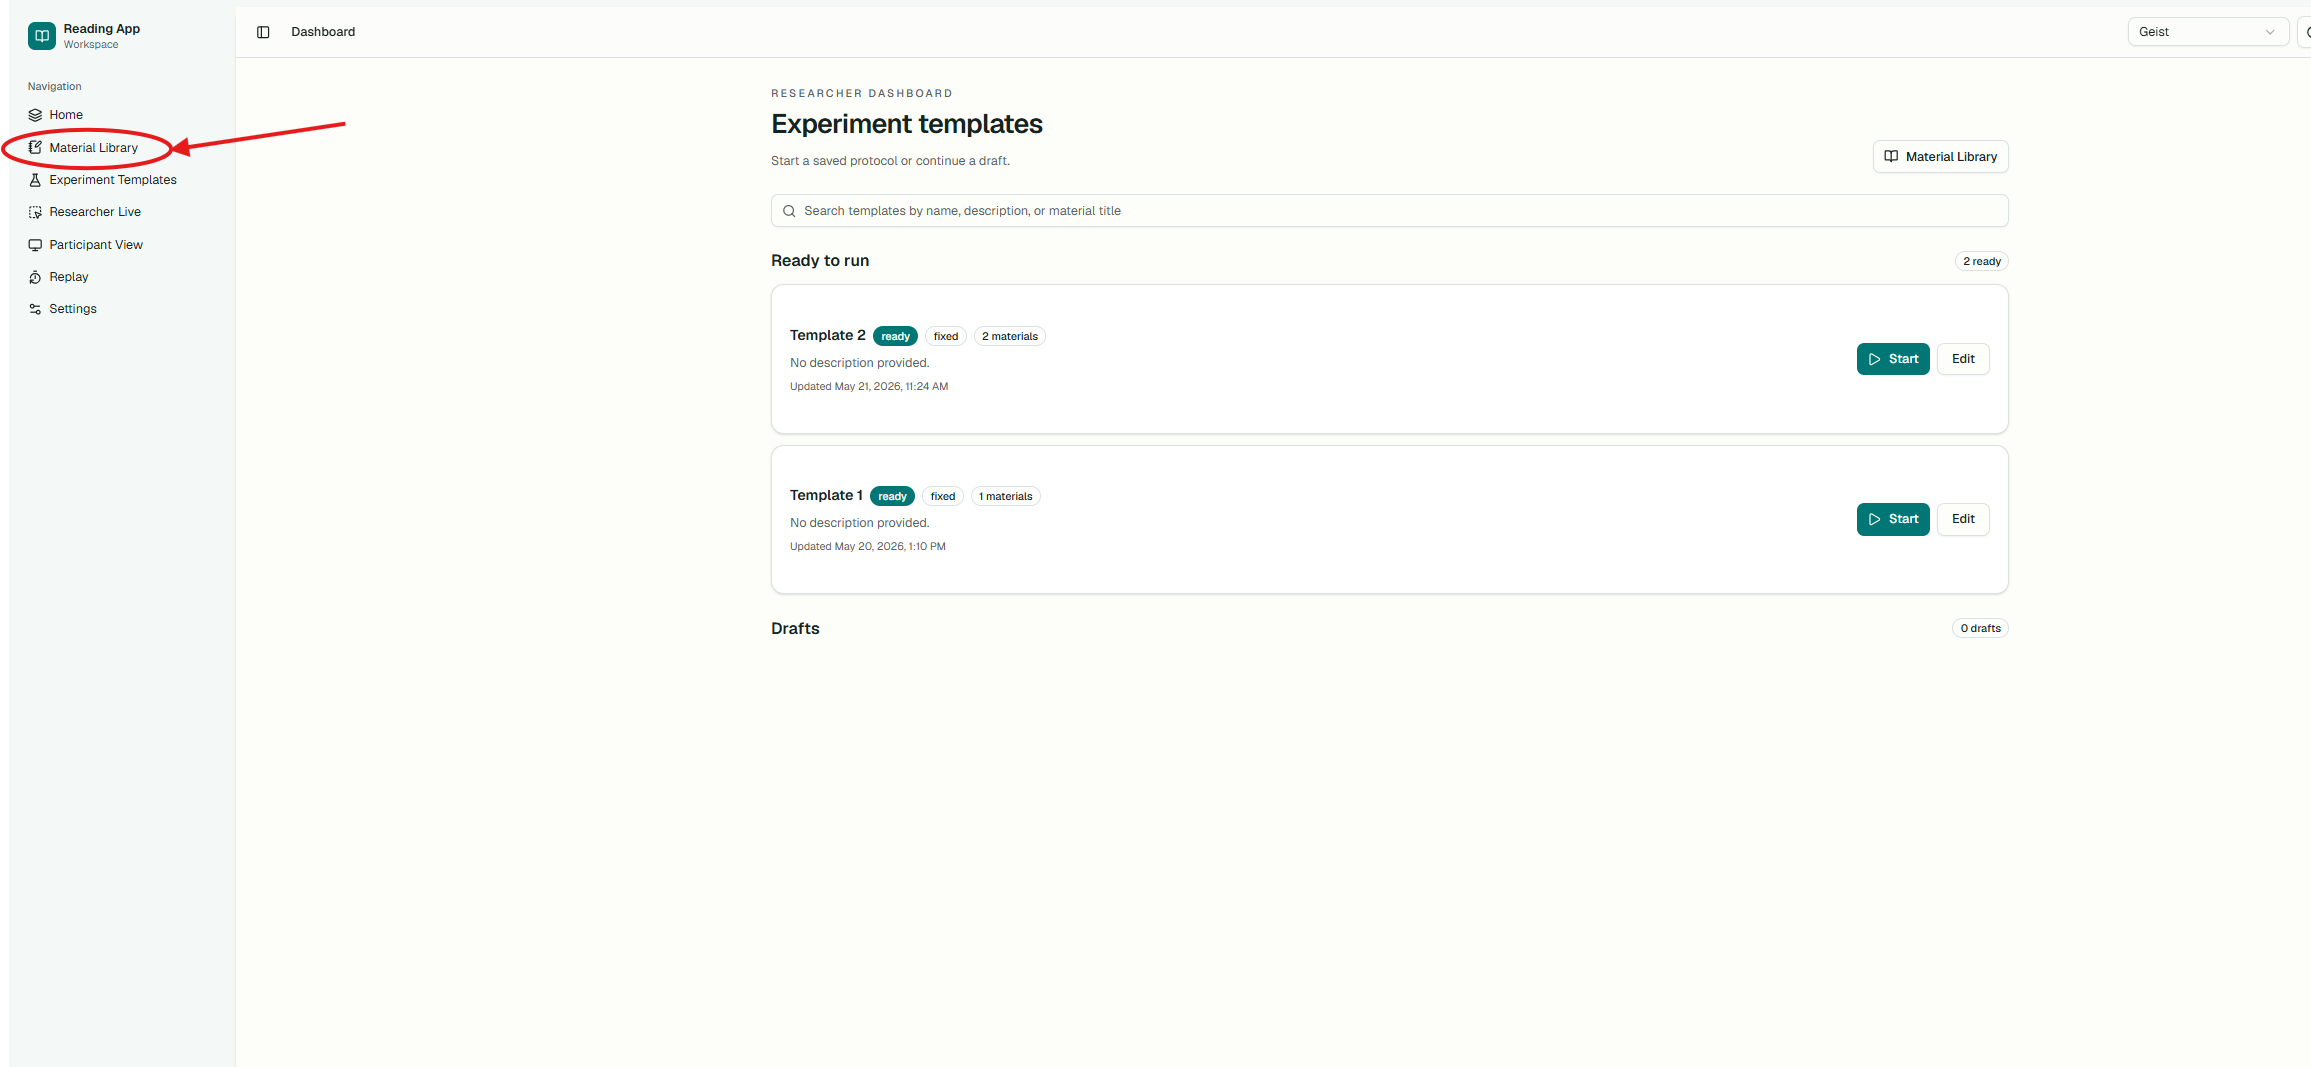
\includegraphics[width=\linewidth,height=0.86\textheight,keepaspectratio]{Backmatter/UserGuideImages/OpenMaterialLibrary.png}}{\guidescreenshotpending{Backmatter/UserGuideImages/OpenMaterialLibrary.png}}
  \caption{Opening the Material Library from the sidebar.}
  \end{figure}
\item
  Click \textbf{New material} (top-right).

\begin{figure}[htbp]
  \centering
\IfFileExists{Backmatter/UserGuideImages/CreateReadingMaterial.png}{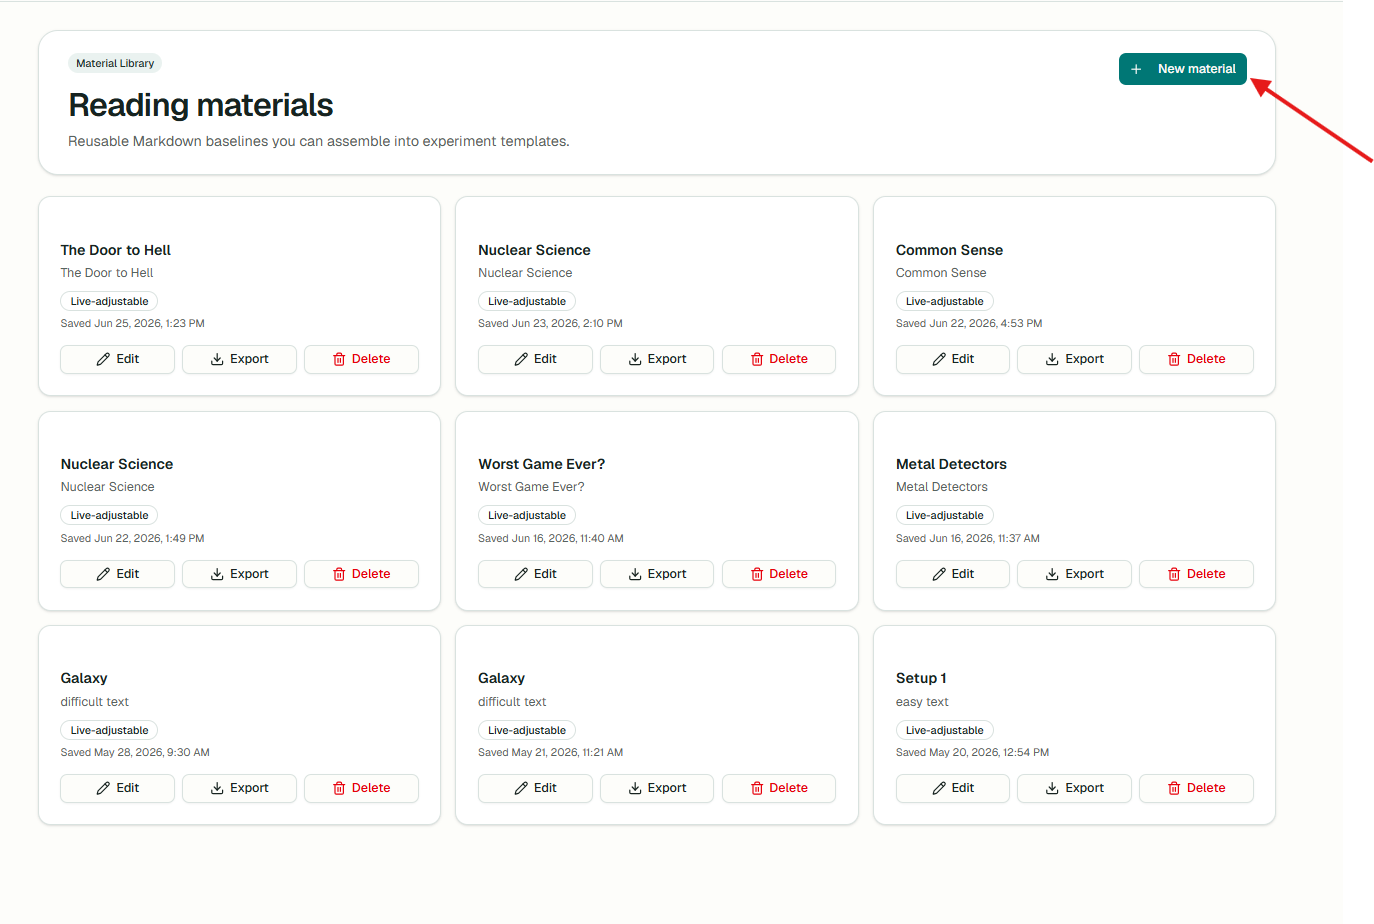
\includegraphics[width=\linewidth,height=0.86\textheight,keepaspectratio]{Backmatter/UserGuideImages/CreateReadingMaterial.png}}{\guidescreenshotpending{Backmatter/UserGuideImages/CreateReadingMaterial.png}}
  \caption{The Material Library listing saved reading materials, with New material at the top right.}
  \end{figure}
\item
  Fill in the \textbf{Reading text} card:

  \begin{itemize}
  \tightlist
  \item
    \textbf{Setup name} --- the internal name shown to researchers (required).
  \item
    \textbf{Text title} --- the title the participant sees (required).
  \item
    \textbf{Markdown text} --- paste your Markdown, or click \textbf{Import .md} to load a file
    (\texttt{.md}, \texttt{.markdown}, \texttt{.txt}). The title can auto-fill from the filename.
  \end{itemize}

\begin{figure}[htbp]
  \centering
\IfFileExists{Backmatter/UserGuideImages/MarkdownPasted.png}{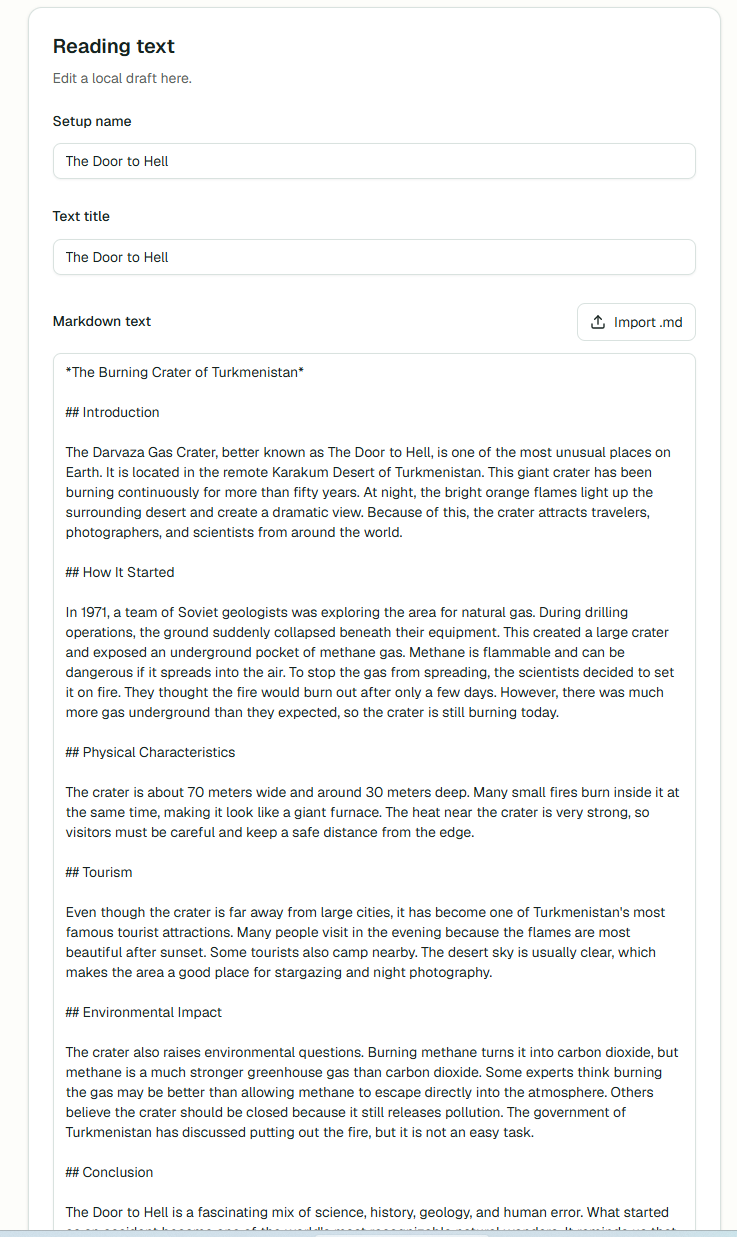
\includegraphics[width=\linewidth,height=0.86\textheight,keepaspectratio]{Backmatter/UserGuideImages/MarkdownPasted.png}}{\guidescreenshotpending{Backmatter/UserGuideImages/MarkdownPasted.png}}
  \caption{The Reading text card with setup name, title, and Markdown pasted in.}
  \end{figure}
\item
  \emph{(Optional)} Add a \textbf{Comprehension quiz}. Each question needs at least two options and one
  marked correct. The quiz is shown to the participant after they finish this text.

\begin{figure}[htbp]
  \centering
\IfFileExists{Backmatter/UserGuideImages/quizEditor.png}{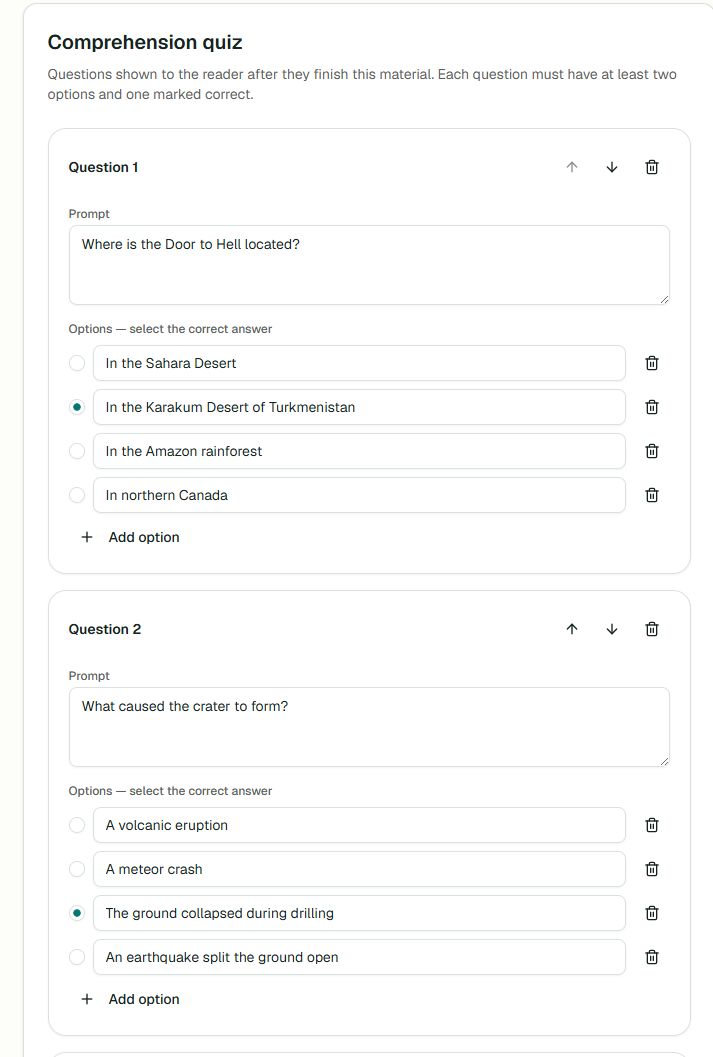
\includegraphics[width=\linewidth,height=0.86\textheight,keepaspectratio]{Backmatter/UserGuideImages/quizEditor.png}}{\guidescreenshotpending{Backmatter/UserGuideImages/quizEditor.png}}
  \caption{The comprehension quiz editor.}
  \end{figure}
\item
  Adjust \textbf{Presentation settings} --- font family, font size, line width, line height, letter
  spacing. Use the \textbf{Live preview} panel on the right to see the participant's reading view
  update as you change values.

\begin{figure}[htbp]
  \centering
\IfFileExists{Backmatter/UserGuideImages/PresentationSettingsWithLivePreview.png}{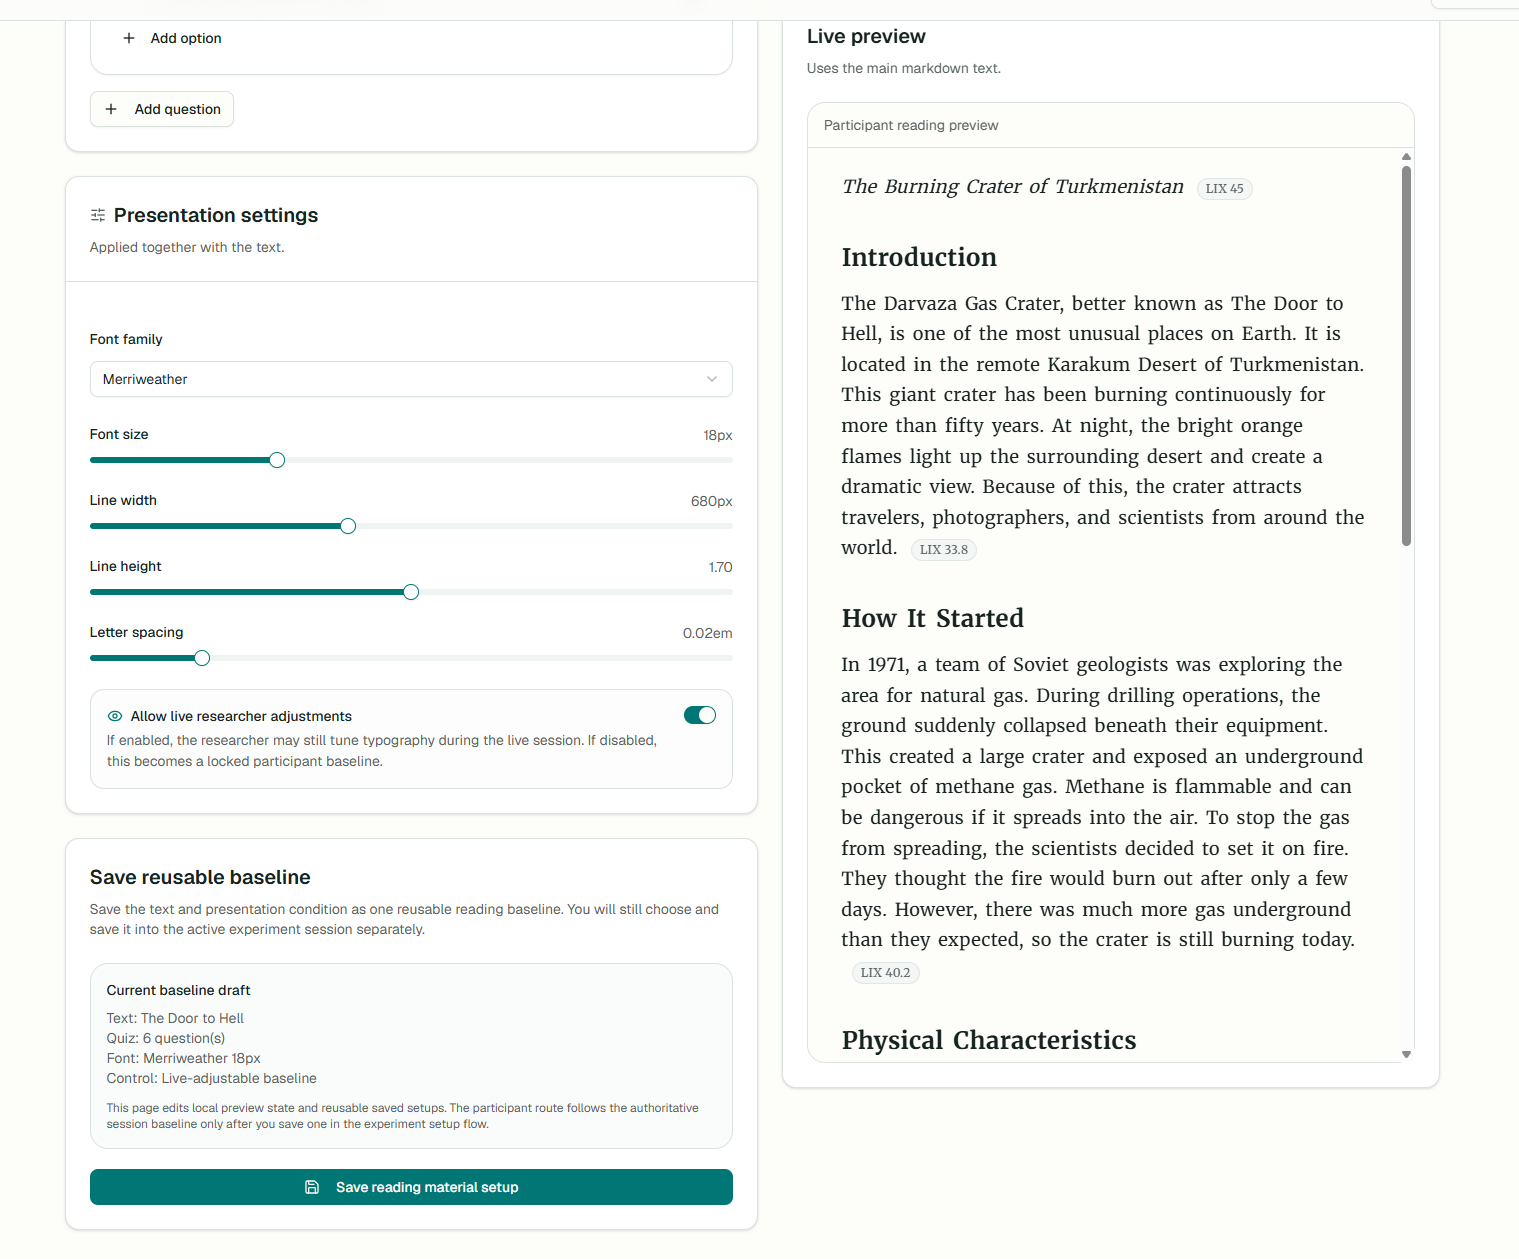
\includegraphics[width=\linewidth,height=0.86\textheight,keepaspectratio]{Backmatter/UserGuideImages/PresentationSettingsWithLivePreview.png}}{\guidescreenshotpending{Backmatter/UserGuideImages/PresentationSettingsWithLivePreview.png}}
  \caption{Presentation settings on the left with the live participant preview on the right.}
  \end{figure}
\item
  Toggle \textbf{Allow live researcher adjustments}:

  \begin{itemize}
  \tightlist
  \item
    \textbf{On} → a \emph{live-adjustable baseline} (the researcher can still tune typography mid-session).
  \item
    \textbf{Off} → a \emph{locked baseline}.
  \end{itemize}
\item
  Click \textbf{Save reading material setup}. You return to the Material Library.
\end{enumerate}

\begin{quote}
\textbf{Import / Export:} Use \textbf{Import JSON} (top-right of the editor) to load a previously
exported material, and the \textbf{Export} button on a library card to download one as
\texttt{*.reading-material.json}.
\end{quote}

\subsection{Build an Experiment Template}\label{52-build-an-experiment-template}

An \emph{experiment template} is a reusable sequence of texts plus presentation defaults, order mode,
runtime strategy, and a calibration requirement.

\begin{enumerate}
\def\labelenumi{\arabic{enumi}.}
\item
  Open \textbf{Experiment Templates} → click \textbf{New template} (or \textbf{Home → continue a draft}).

\begin{figure}[htbp]
  \centering
\IfFileExists{Backmatter/UserGuideImages/ExperimentTemplateLibrary.png}{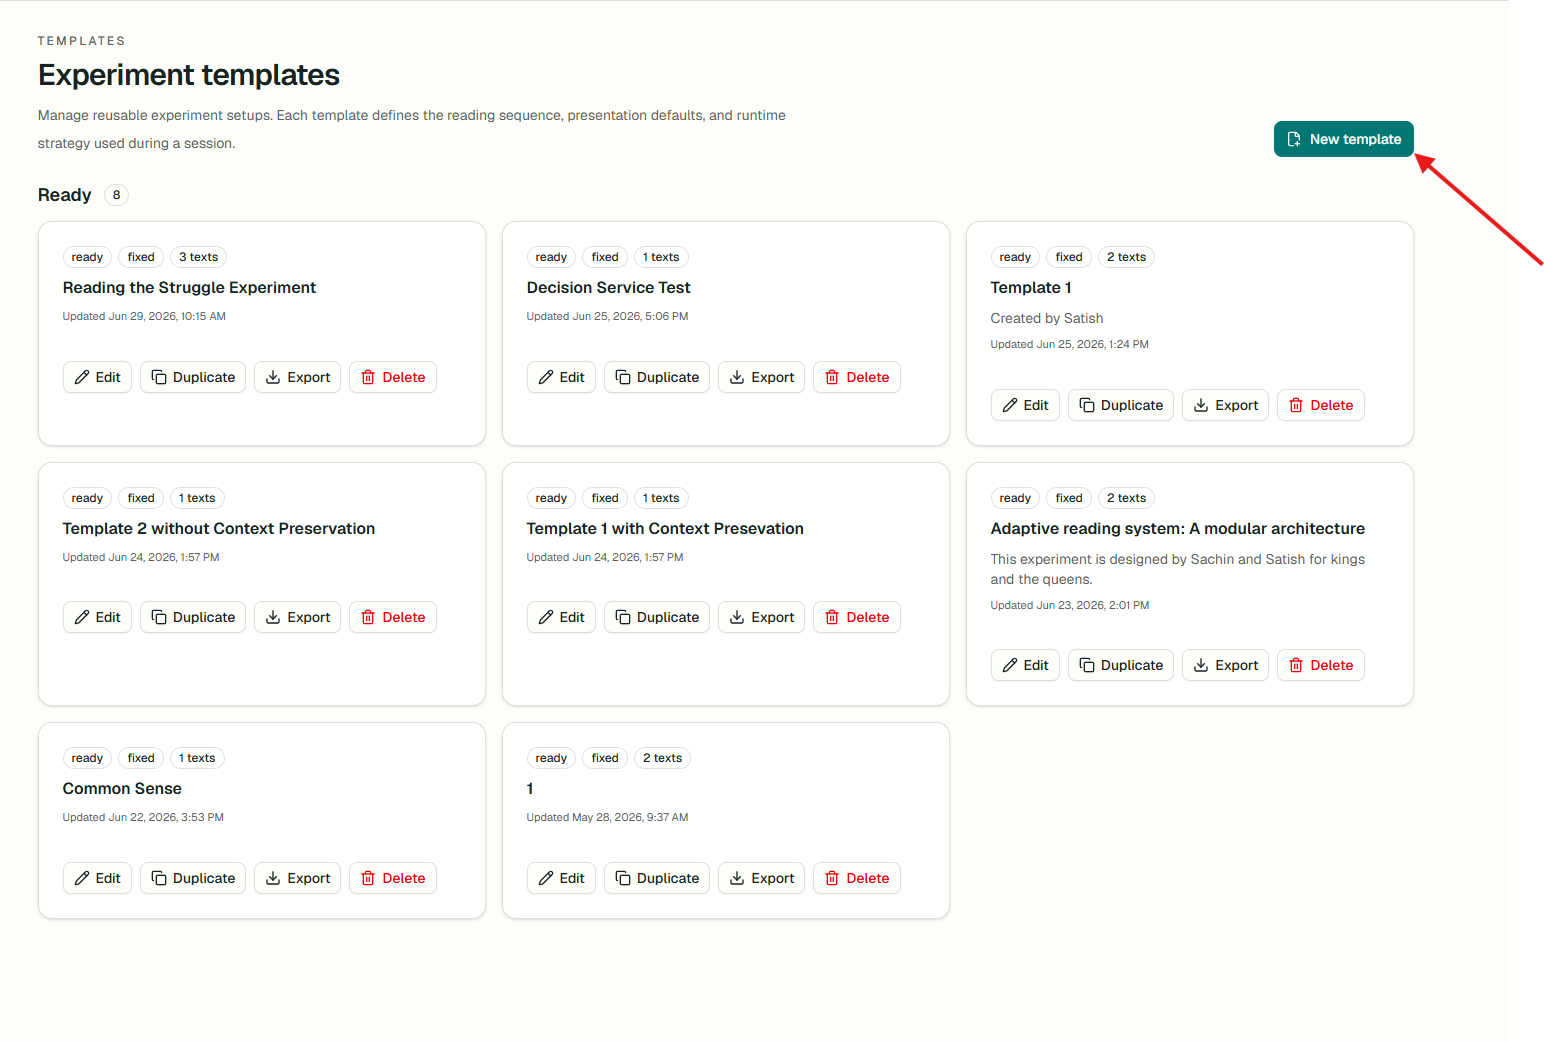
\includegraphics[width=\linewidth,height=0.86\textheight,keepaspectratio]{Backmatter/UserGuideImages/ExperimentTemplateLibrary.png}}{\guidescreenshotpending{Backmatter/UserGuideImages/ExperimentTemplateLibrary.png}}
  \caption{The Experiment Templates library (ready, drafts, archived).}
  \end{figure}
\item
  In \textbf{Template settings}, set:

  \begin{itemize}
  \tightlist
  \item
    \textbf{Template name} (required) and an optional \textbf{Description}.
  \item
    \textbf{Status} --- \texttt{Draft}, \texttt{Ready}, or \texttt{Archived}. Only \textbf{Ready} templates can be started from Home.
  \item
    \textbf{Material order} --- \texttt{Fixed\ order} or \texttt{Fully\ random\ at\ session\ start}.
  \item
    \textbf{Decision strategy} --- the runtime decision plugin/mode (see \cref{8-runtime-plugins-decision--eye-analysis}).
  \item
    \textbf{Require calibration} --- keep enabled for real eye-tracker sessions.
  \item
    \textbf{Default font / size / line width / live adjustments} --- applied as defaults to added texts.
  \end{itemize}

\begin{figure}[htbp]
  \centering
\IfFileExists{Backmatter/UserGuideImages/ExperimentTemplate.png}{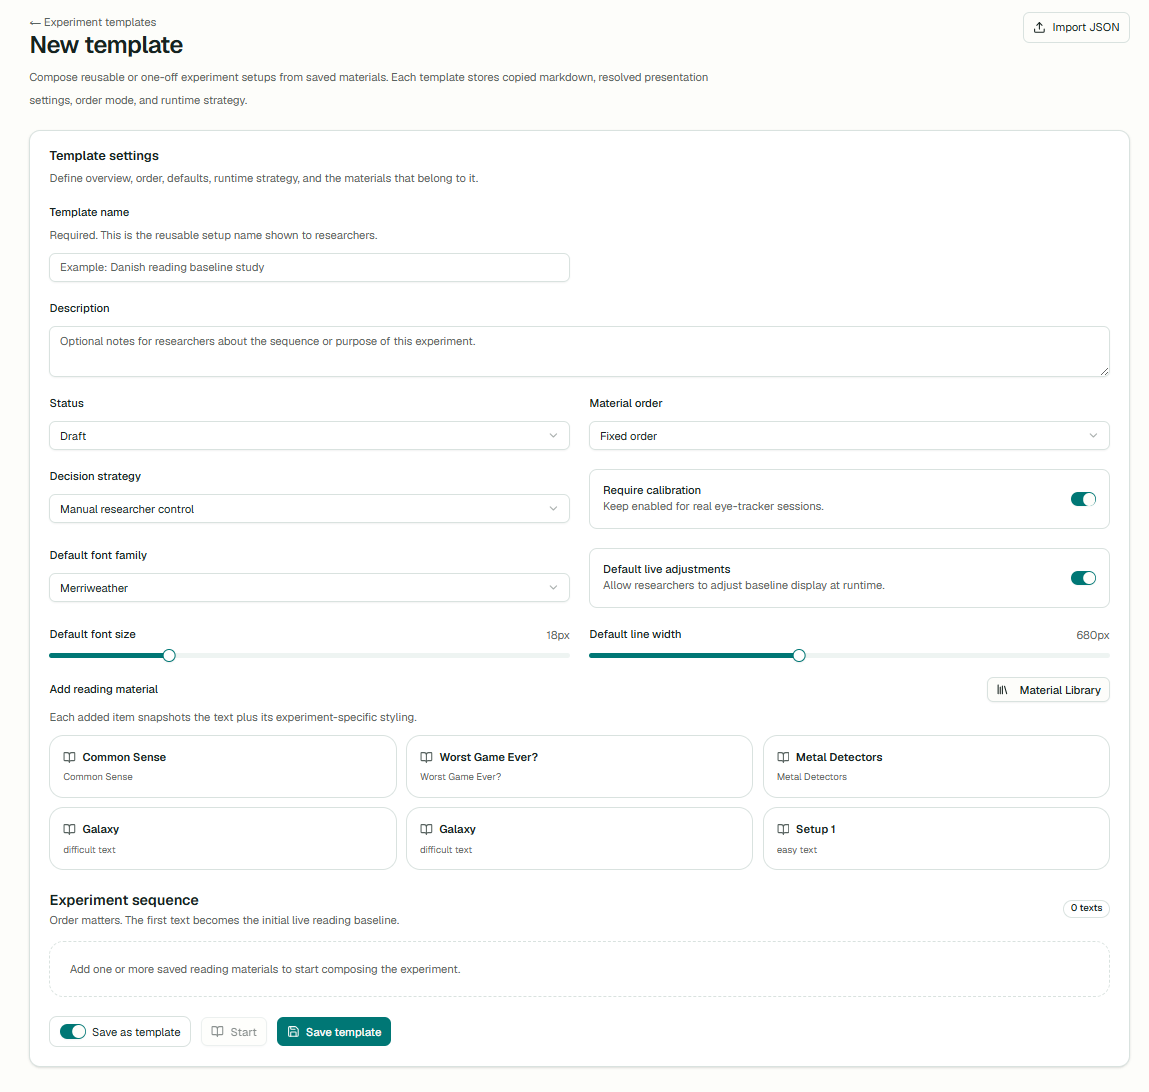
\includegraphics[width=\linewidth,height=0.86\textheight,keepaspectratio]{Backmatter/UserGuideImages/ExperimentTemplate.png}}{\guidescreenshotpending{Backmatter/UserGuideImages/ExperimentTemplate.png}}
  \caption{The New template editor: template settings, defaults, and the reading-material picker.}
  \end{figure}
\item
  Under \textbf{Add reading material}, click any saved material to add it to the sequence. Each added
  item \emph{snapshots} the text and its styling into the template.

\begin{figure}[htbp]
  \centering
\IfFileExists{Backmatter/UserGuideImages/MaterialPikcerGrid.png}{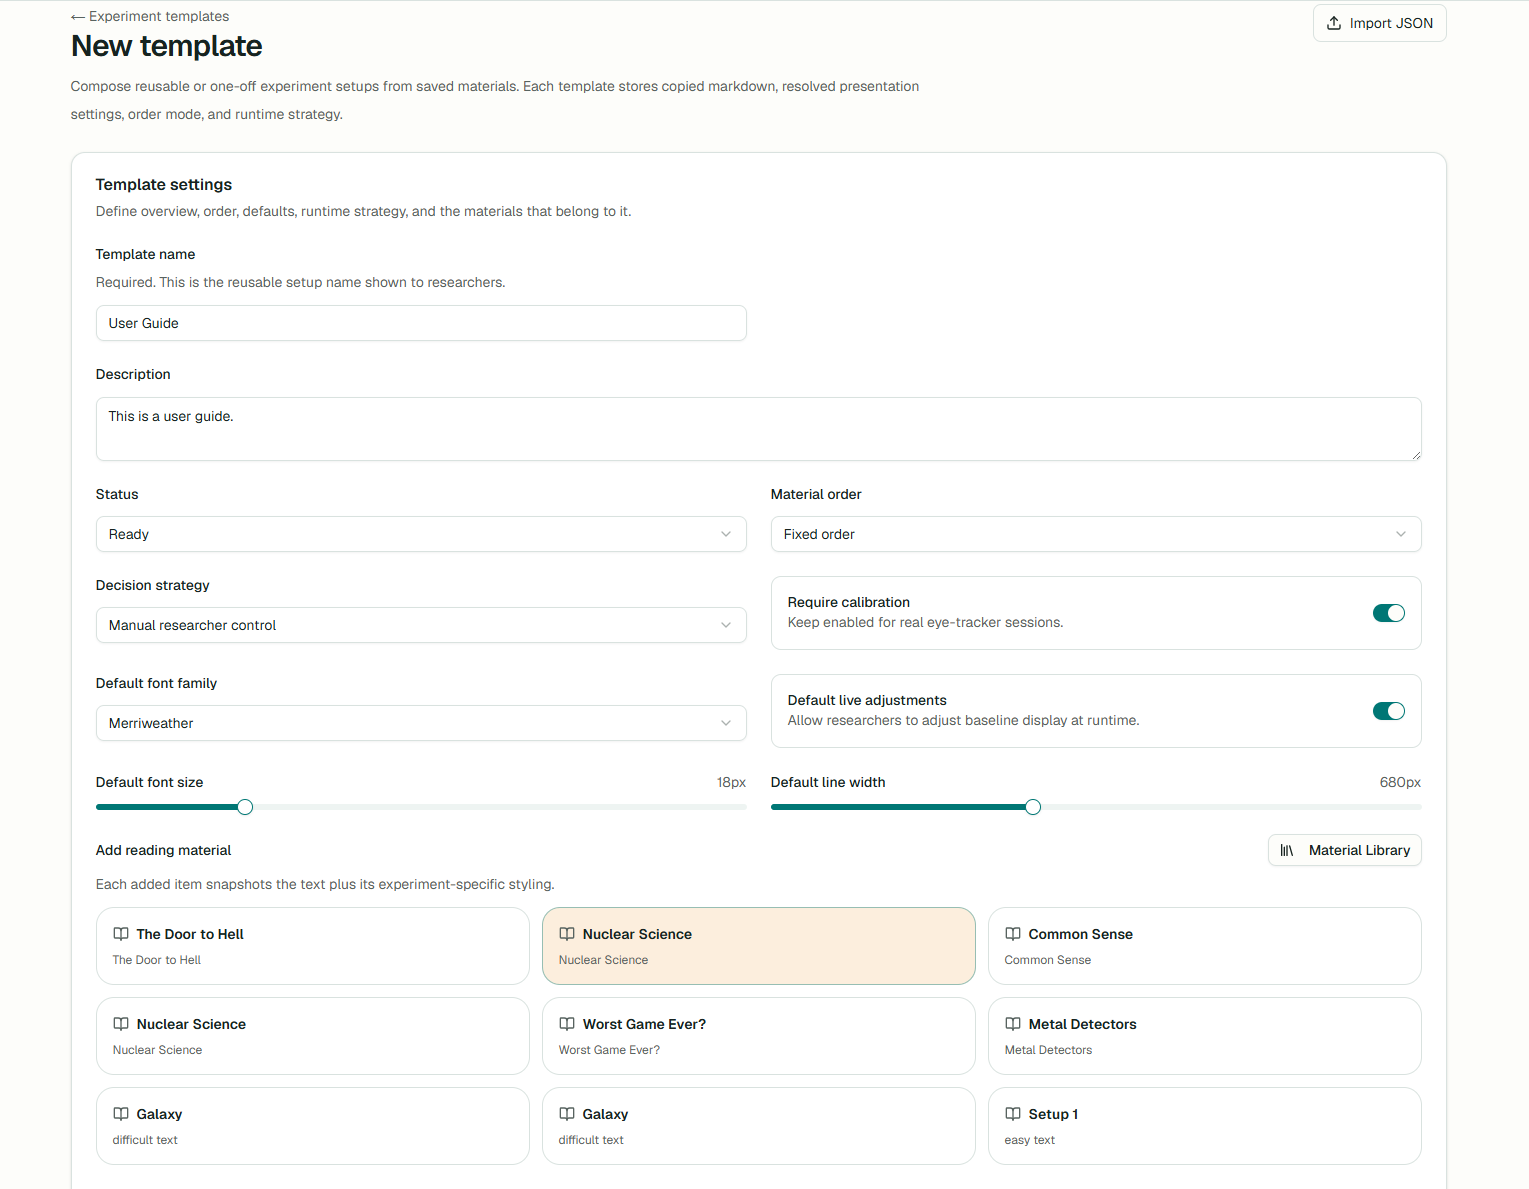
\includegraphics[width=\linewidth,height=0.86\textheight,keepaspectratio]{Backmatter/UserGuideImages/MaterialPikcerGrid.png}}{\guidescreenshotpending{Backmatter/UserGuideImages/MaterialPikcerGrid.png}}
  \caption{The reading-material picker grid for adding texts to the template.}
  \end{figure}
\item
  Arrange the \textbf{Experiment sequence}:

  \begin{itemize}
  \tightlist
  \item
    The \textbf{first text becomes the initial live reading baseline}.
  \item
    Use the up/down arrows to reorder, the trash icon to remove.
  \item
    Per text, override \textbf{displayed title, font, size, line width, line height, letter spacing}, and
    \textbf{Allow live presentation adjustments}.
  \end{itemize}

\begin{figure}[htbp]
  \centering
\IfFileExists{Backmatter/UserGuideImages/ExperiementSequence.png}{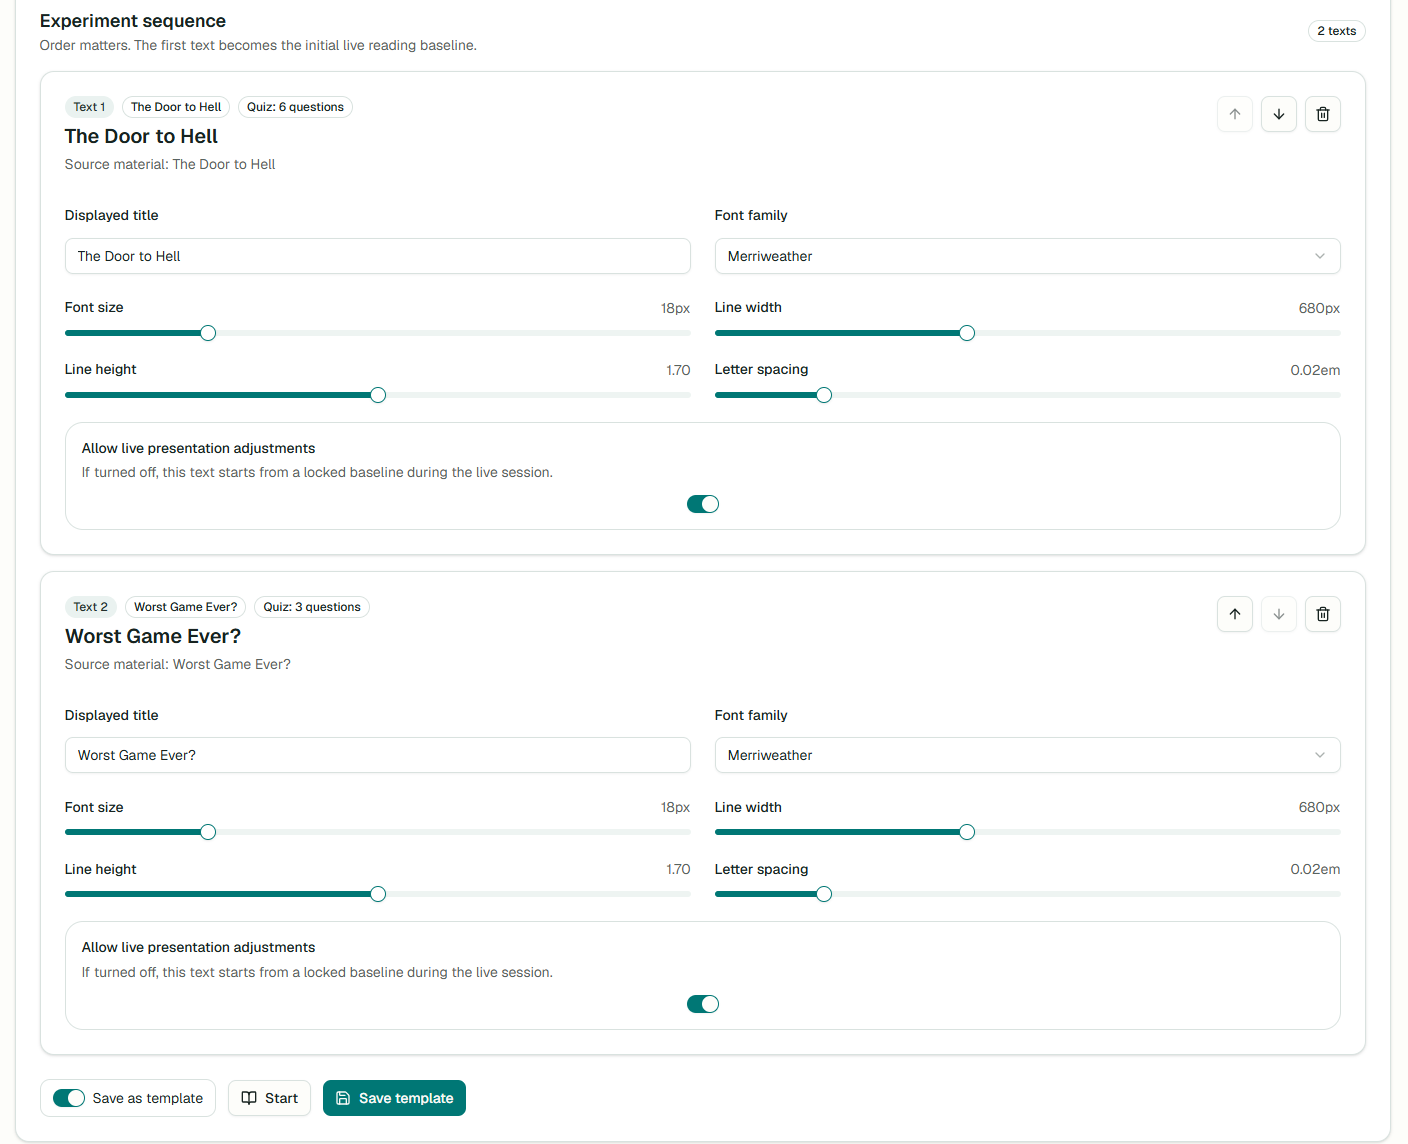
\includegraphics[width=\linewidth,height=0.86\textheight,keepaspectratio]{Backmatter/UserGuideImages/ExperiementSequence.png}}{\guidescreenshotpending{Backmatter/UserGuideImages/ExperiementSequence.png}}
  \caption{The experiment sequence: ordered text cards with per-text presentation overrides.}
  \end{figure}
\item
  Finish:

  \begin{itemize}
  \tightlist
  \item
    \textbf{Save template} (or \textbf{Update template}) --- keeps you in the library.
  \item
    \textbf{Start} --- saves and jumps straight into a session for this template. (Turn off \textbf{Save as
    template} first if you want a one-off run that is not stored.)
  \end{itemize}
\end{enumerate}

\begin{quote}
\textbf{Duplicate / Export:} From the template library, use \textbf{Duplicate} to clone a setup as a new
draft, or \textbf{Export} to download it as \texttt{*.experiment-template.json}. \textbf{Import JSON} is at the
top-right of the template editor.
\end{quote}

\subsection{Run an Experiment Session}\label{53-run-an-experiment-session}

Sessions are driven by a \textbf{4-step stepper}. The researcher completes Steps 1--2 (preparation); the
participant completes Steps 3--4. Start a session by clicking \textbf{Start} on a ready template (Home),
or \textbf{Start} from the template editor.

\begin{figure}[htbp]
\centering
\IfFileExists{Backmatter/UserGuideImages/StartExperiment.png}{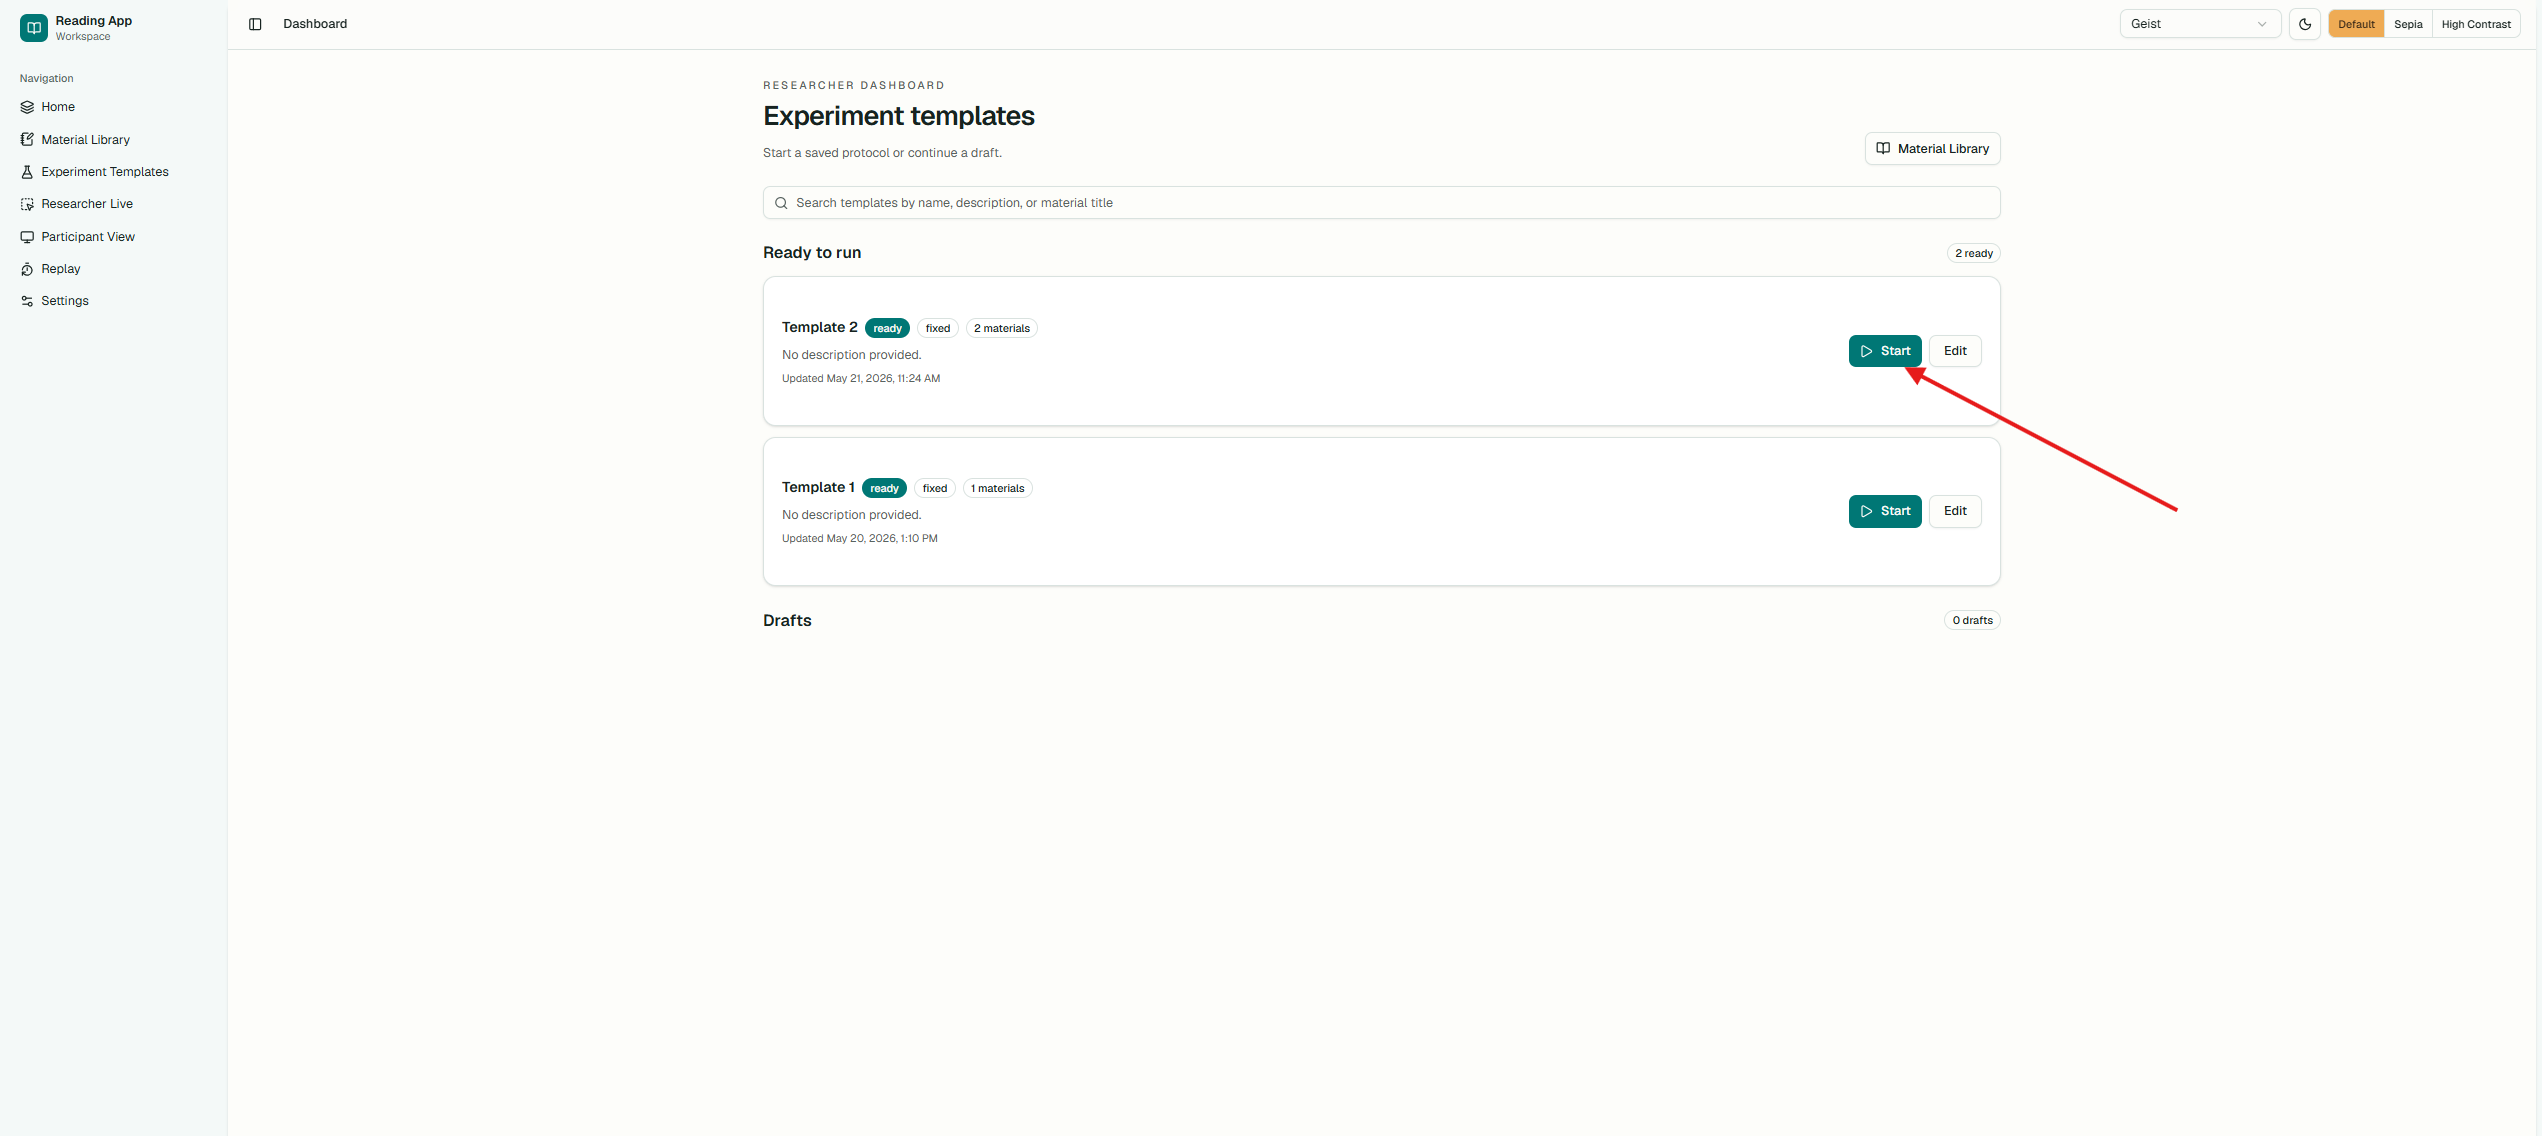
\includegraphics[width=\linewidth,height=0.86\textheight,keepaspectratio]{Backmatter/UserGuideImages/StartExperiment.png}}{\guidescreenshotpending{Backmatter/UserGuideImages/StartExperiment.png}}
\caption{Start a session by clicking Start on a ready template from the dashboard.}
\end{figure}

The left rail shows all four steps with status badges (\texttt{Done}, \texttt{Current}, \texttt{Available}, \texttt{Locked})
and an owner badge (Researcher / Participant).

\subsubsection{\texorpdfstring{Step 1 --- Choose eyetracker \emph{(Researcher)}}{Step 1 --- Choose eyetracker (Researcher)}}\label{step-1--choose-eyetracker-researcher}

\begin{quote}
This step's content depends on the active \textbf{input mode} (Settings → Input mode). In \textbf{Mouse
mode} it shows a ``Mouse input is active'' card and completes automatically. The steps below
describe full \textbf{Eyetracker} mode (also used for \textbf{Eyetracker + face}).
\end{quote}

\begin{enumerate}
\def\labelenumi{\arabic{enumi}.}
\item
  Pick the device from the \textbf{eyetracker} dropdown (shown as \emph{name / model / serial}). Click the
  refresh icon to re-scan if your device is missing.
\item
  Upload the device \textbf{licence} file (drag-and-drop or browse). Optionally tick \textbf{save licence}
  and/or \textbf{overwrite existing licence}.
\item
  Confirm the selection. Click \textbf{Save researcher setup} to continue.

\begin{figure}[htbp]
  \centering
\IfFileExists{Backmatter/UserGuideImages/Stepper1.png}{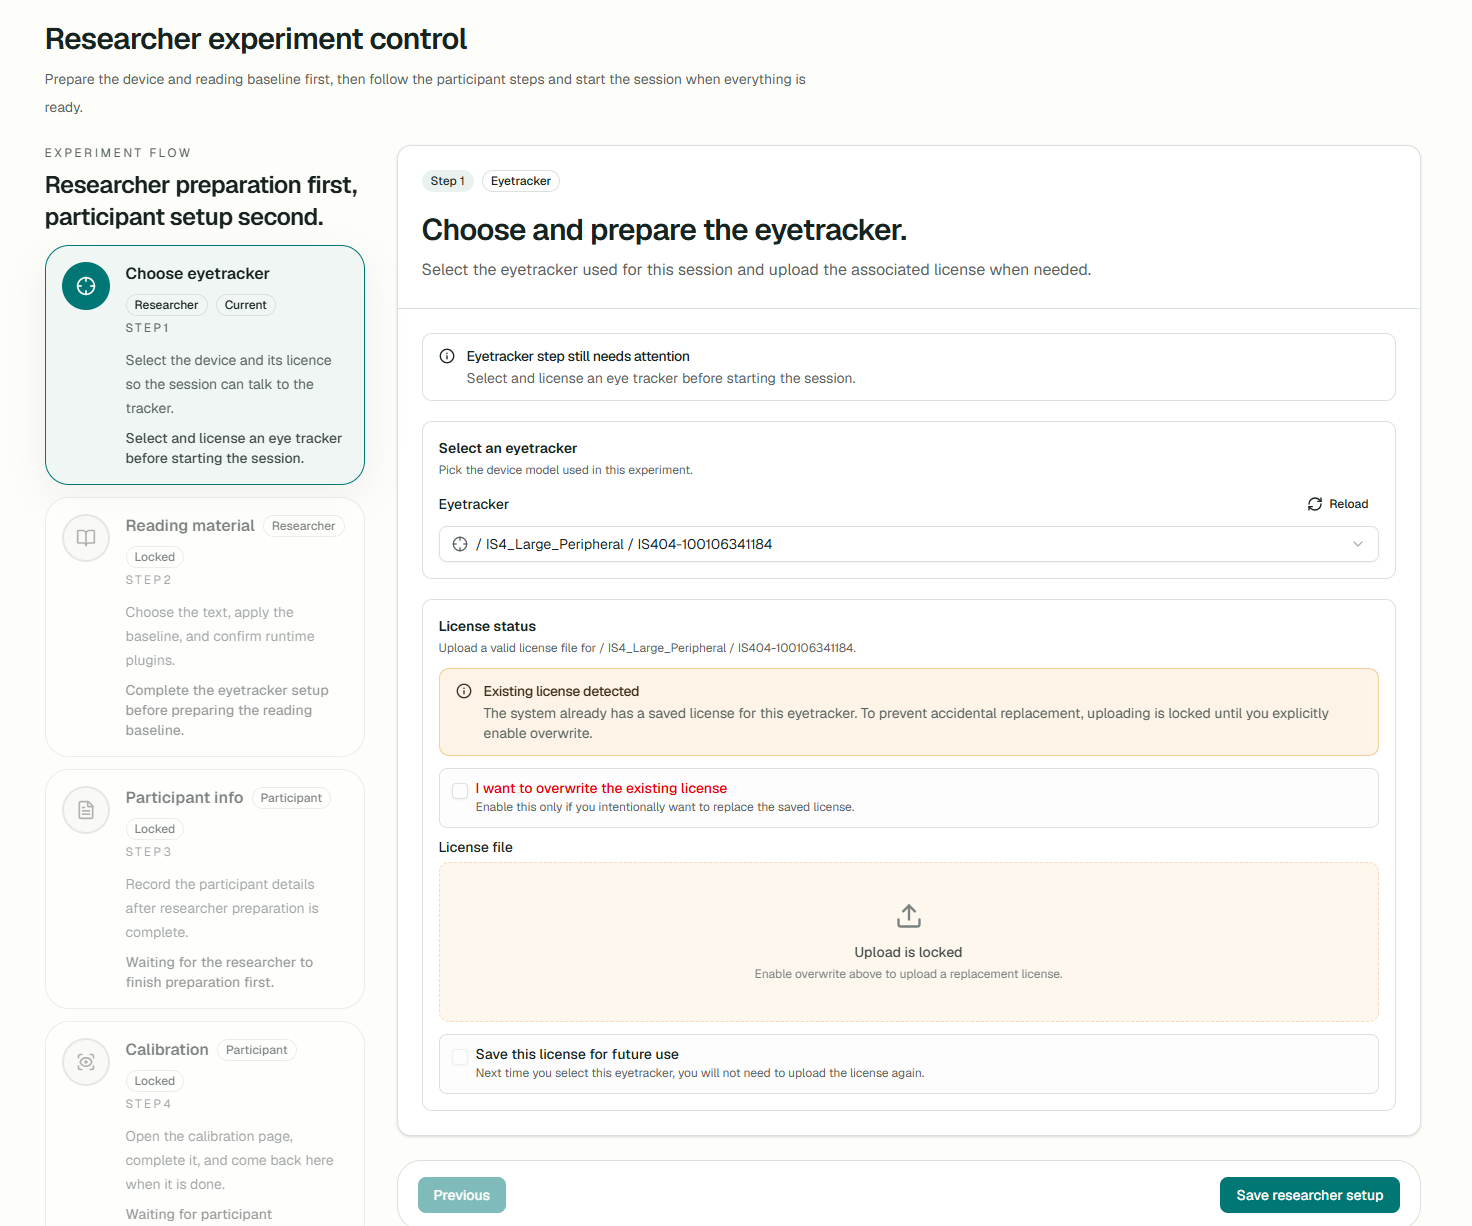
\includegraphics[width=\linewidth,height=0.86\textheight,keepaspectratio]{Backmatter/UserGuideImages/Stepper1.png}}{\guidescreenshotpending{Backmatter/UserGuideImages/Stepper1.png}}
  \caption{Step 1: choosing and preparing the eyetracker, including licence upload.}
  \end{figure}
\end{enumerate}

\subsubsection{\texorpdfstring{Step 2 --- Reading material \emph{(Researcher)}}{Step 2 --- Reading material (Researcher)}}\label{step-2--reading-material-researcher}

\begin{enumerate}
\def\labelenumi{\arabic{enumi}.}
\item
  Pick a \textbf{reusable experiment} (Ready templates appear as cards). Its first text becomes the
  live reading baseline. \emph{(If you started from a template, this selection is locked.)}
\item
  Confirm the \textbf{Runtime plugins}:

  \begin{itemize}
  \tightlist
  \item
    \textbf{Decision plugin} --- Manual / Rule-based (advisory or autonomous) / external Decision-maker.
  \item
    \textbf{Eye analyzer} --- Built-in analyzer or an external Eye analyzer service.
  \item
    Status badges show whether each external service is \emph{Connected}, \emph{Built-in}, or \emph{Unavailable}.
  \end{itemize}
\item
  Review the selection summary, then click \textbf{Apply baseline \& continue}.

\begin{figure}[htbp]
  \centering
\IfFileExists{Backmatter/UserGuideImages/Step2.png}{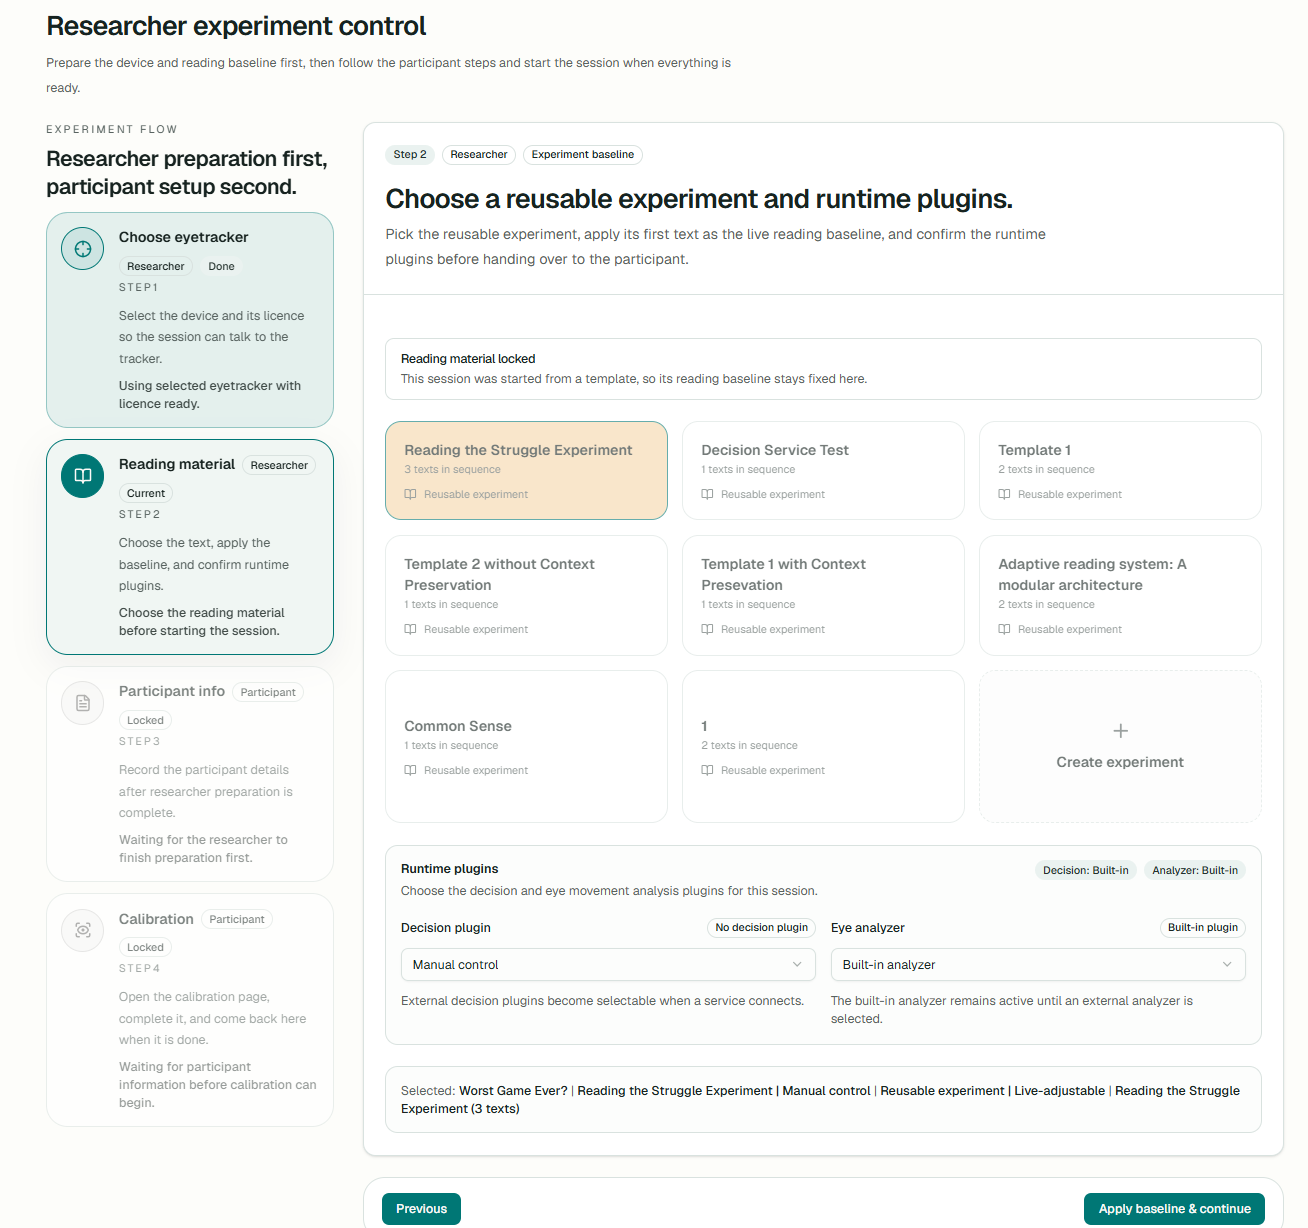
\includegraphics[width=\linewidth,height=0.86\textheight,keepaspectratio]{Backmatter/UserGuideImages/Step2.png}}{\guidescreenshotpending{Backmatter/UserGuideImages/Step2.png}}
  \caption{Step 2: selecting a reusable experiment and confirming the runtime plugins.}
  \end{figure}
\end{enumerate}

\subsubsection{\texorpdfstring{Step 3 --- Participant info \emph{(Participant)}}{Step 3 --- Participant info (Participant)}}\label{step-3--participant-info-participant}

Recorded on the participant's screen (or by the researcher). Fields: \textbf{Name, Age, Sex, Existing eye
condition, Reading proficiency}. All are required and validated. Click \textbf{Continue to calibration}.

\begin{figure}[htbp]
\centering
\IfFileExists{Backmatter/UserGuideImages/Step3.png}{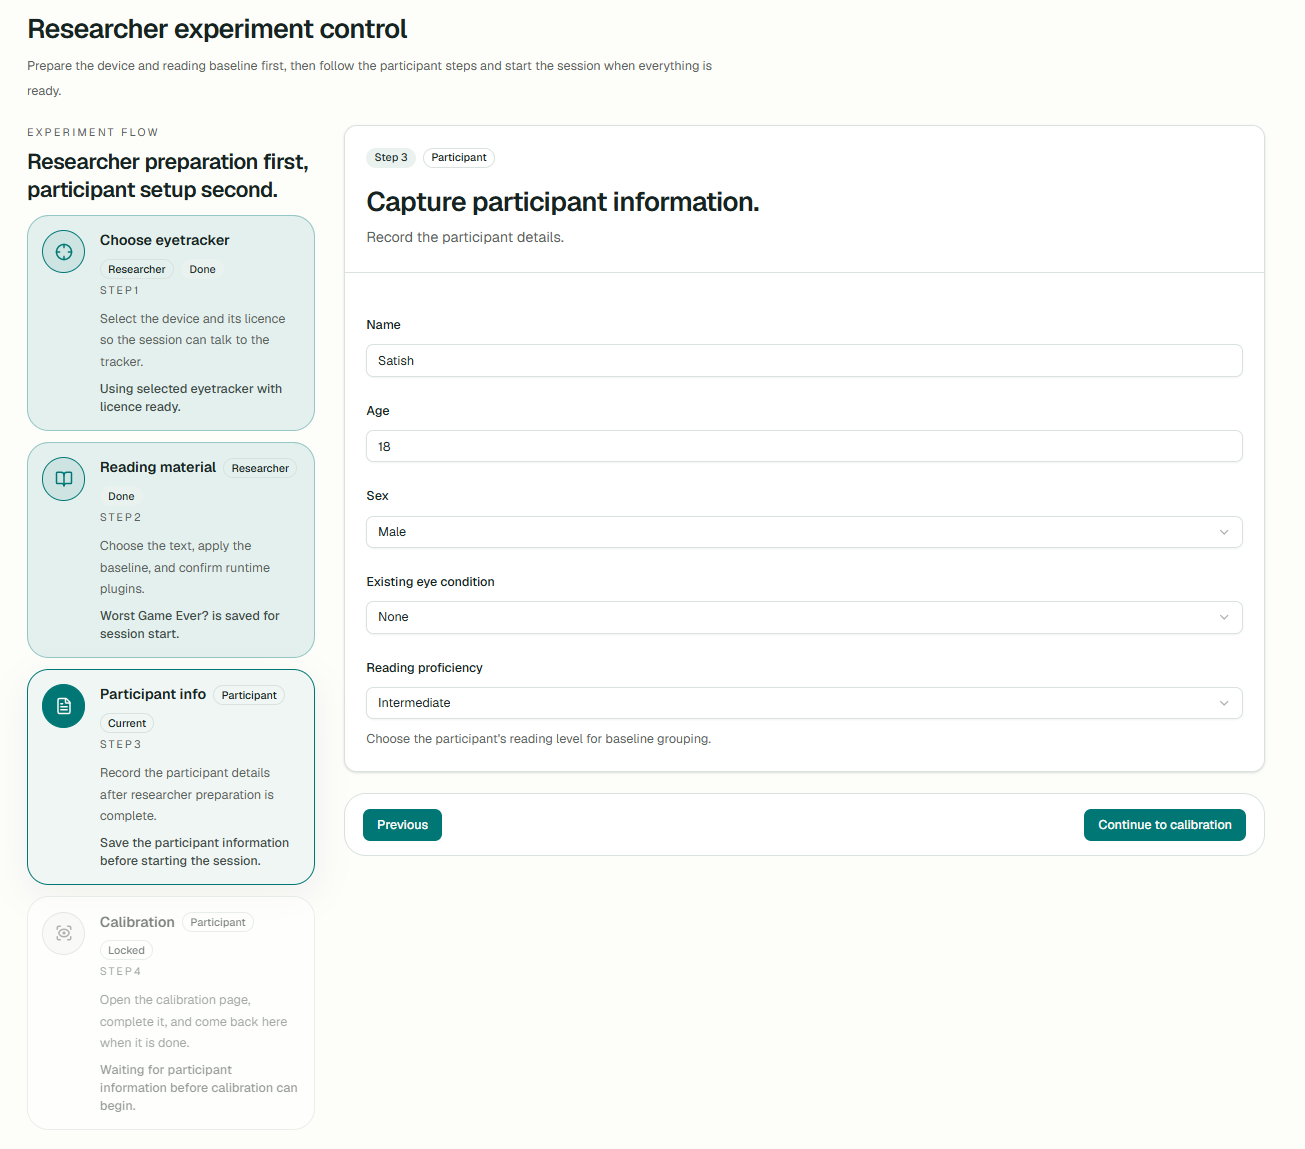
\includegraphics[width=\linewidth,height=0.86\textheight,keepaspectratio]{Backmatter/UserGuideImages/Step3.png}}{\guidescreenshotpending{Backmatter/UserGuideImages/Step3.png}}
\caption{Step 3: the participant information form.}
\end{figure}

\subsubsection{\texorpdfstring{Step 4 --- Calibration \emph{(Participant)}}{Step 4 --- Calibration (Participant)}}\label{step-4--calibration-participant}

Opens the full-screen calibration routine. See \cref{55-calibration}. When validation passes, the
participant returns here automatically.

\subsubsection{Start the session}\label{start-the-session}

Once all four steps show \textbf{Done}, the final button becomes \textbf{Start reading session}. Clicking it:
- (Researcher start) → opens \textbf{Researcher Live}.
- (Participant start) → opens the \textbf{Reading} page on the participant screen.

\begin{figure}[htbp]
\centering
\IfFileExists{Backmatter/UserGuideImages/Stepper4.png}{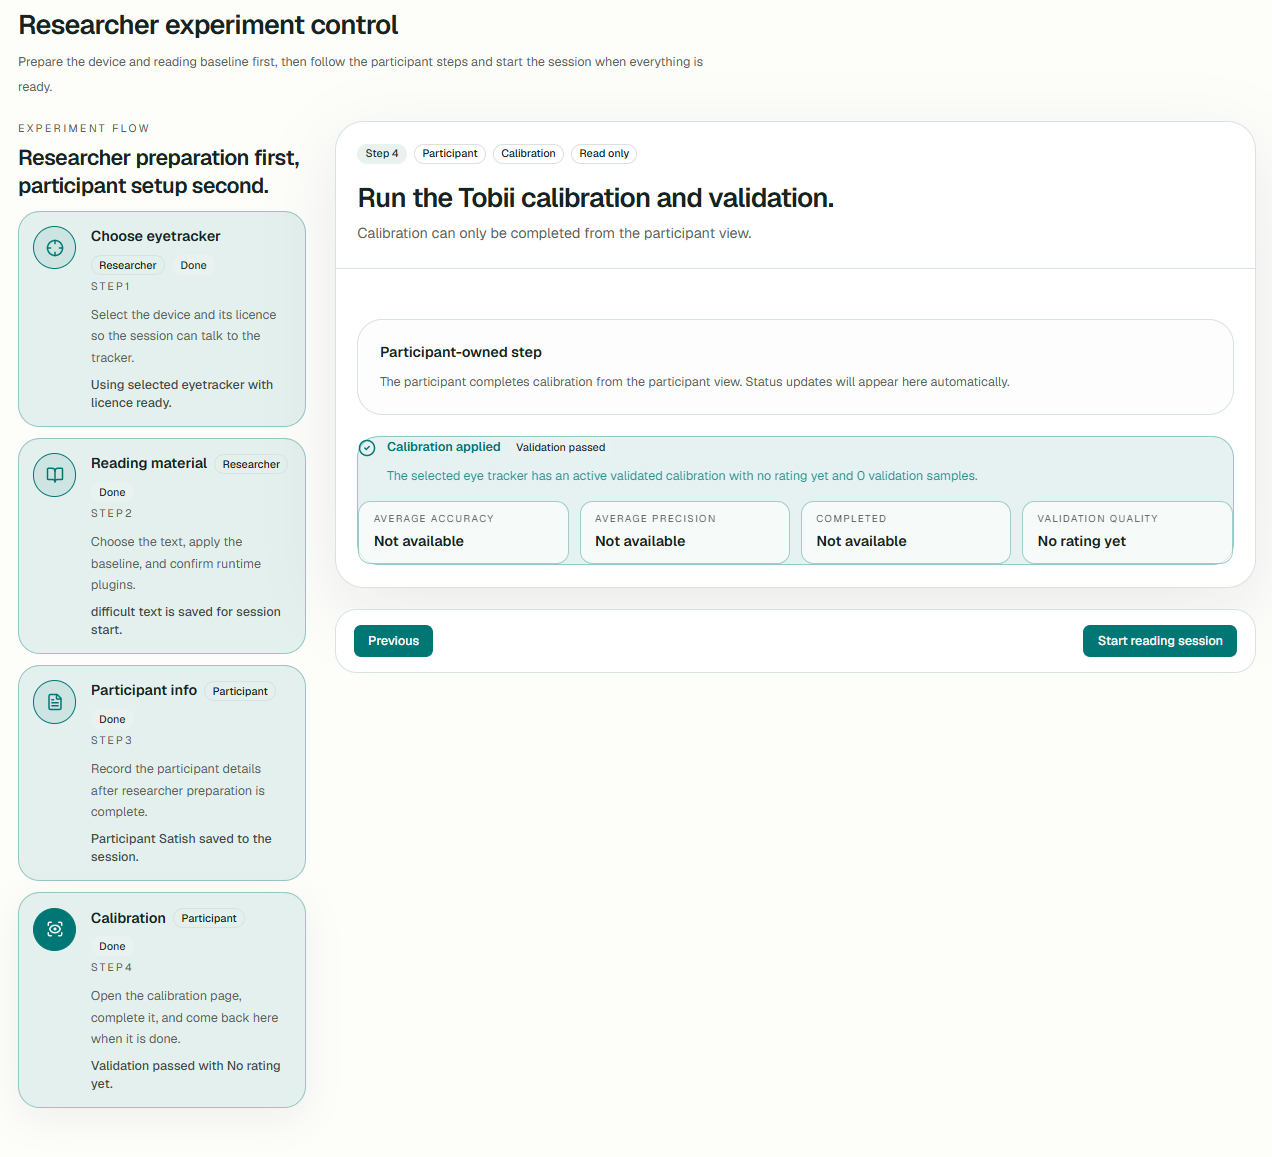
\includegraphics[width=\linewidth,height=0.86\textheight,keepaspectratio]{Backmatter/UserGuideImages/Stepper4.png}}{\guidescreenshotpending{Backmatter/UserGuideImages/Stepper4.png}}
\caption{All four steps complete, with the reading session ready to start.}
\end{figure}

\subsection{The Participant View}\label{54-the-participant-view}

Open \textbf{Participant View} from the sidebar (it opens in a new tab) and place it on the
participant's screen.

\begin{itemize}
\item
  Before the researcher begins setup, the page shows a \textbf{waiting} card (``Experiment has not
  started yet'' / ``Your session is being prepared'').

\begin{figure}[htbp]
  \centering
\IfFileExists{Backmatter/UserGuideImages/ExperimentNotStarted.png}{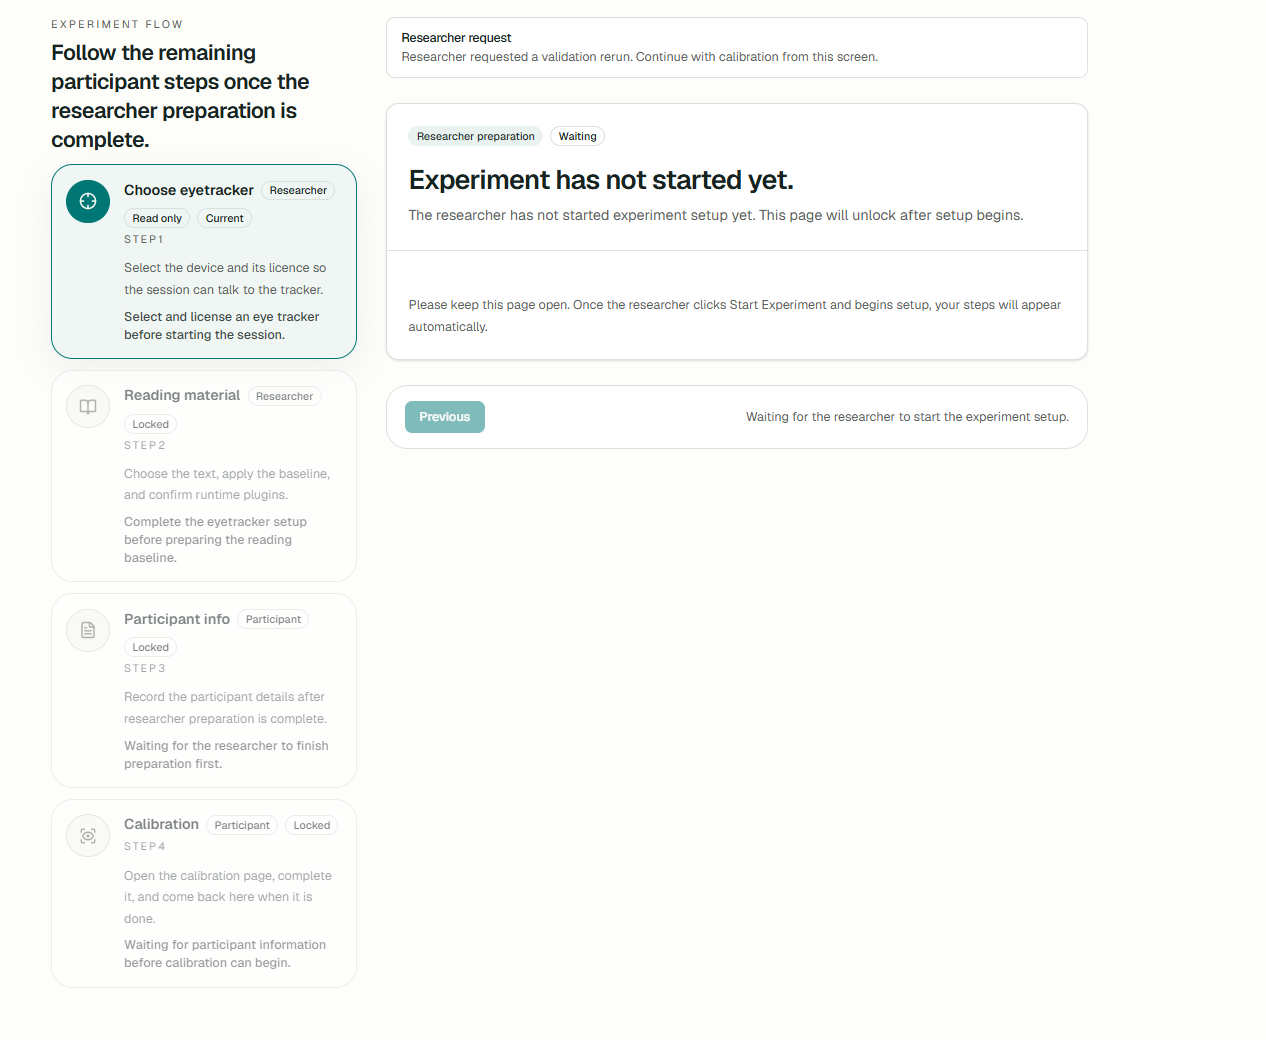
\includegraphics[width=\linewidth,height=0.86\textheight,keepaspectratio]{Backmatter/UserGuideImages/ExperimentNotStarted.png}}{\guidescreenshotpending{Backmatter/UserGuideImages/ExperimentNotStarted.png}}
  \caption{The participant view before the researcher has started setup (``Experiment has not started yet'').}
  \end{figure}

\begin{figure}[htbp]
  \centering
\IfFileExists{Backmatter/UserGuideImages/SessionBeingReady.png}{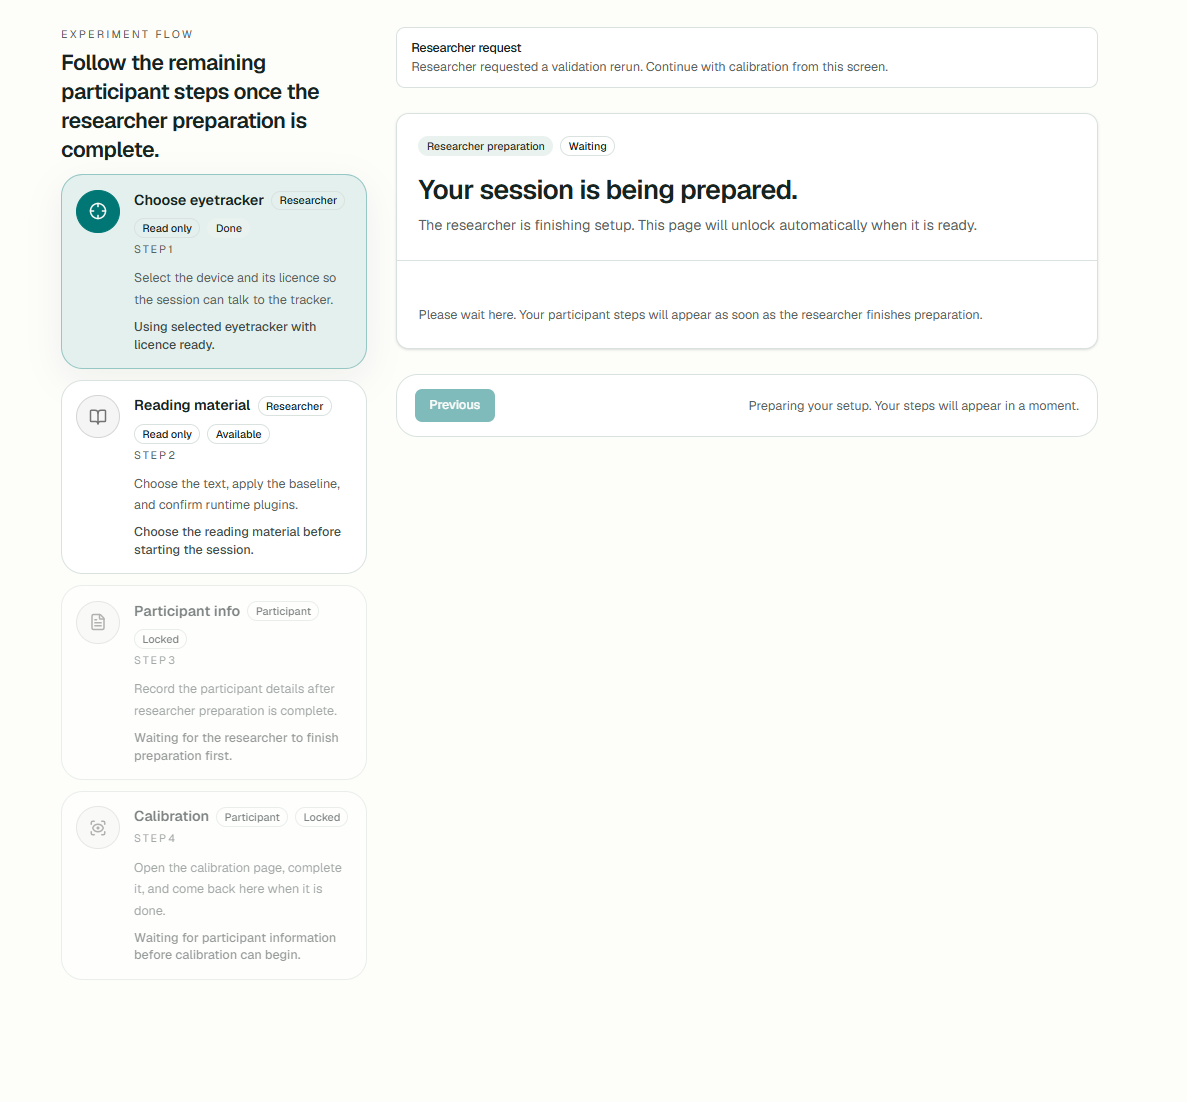
\includegraphics[width=\linewidth,height=0.86\textheight,keepaspectratio]{Backmatter/UserGuideImages/SessionBeingReady.png}}{\guidescreenshotpending{Backmatter/UserGuideImages/SessionBeingReady.png}}
  \caption{Once the researcher begins setup, the participant sees ``Your session is being prepared''.}
  \end{figure}
\item
  Once researcher preparation (Steps 1--2) is ready, the participant's steps (3--4) unlock
  automatically.
\item
  After participant info and calibration are complete, the page shows \textbf{``Waiting for the
  researcher to start the session.''}

\begin{figure}[htbp]
  \centering
\IfFileExists{Backmatter/UserGuideImages/ParticipantWaitingScreen.png}{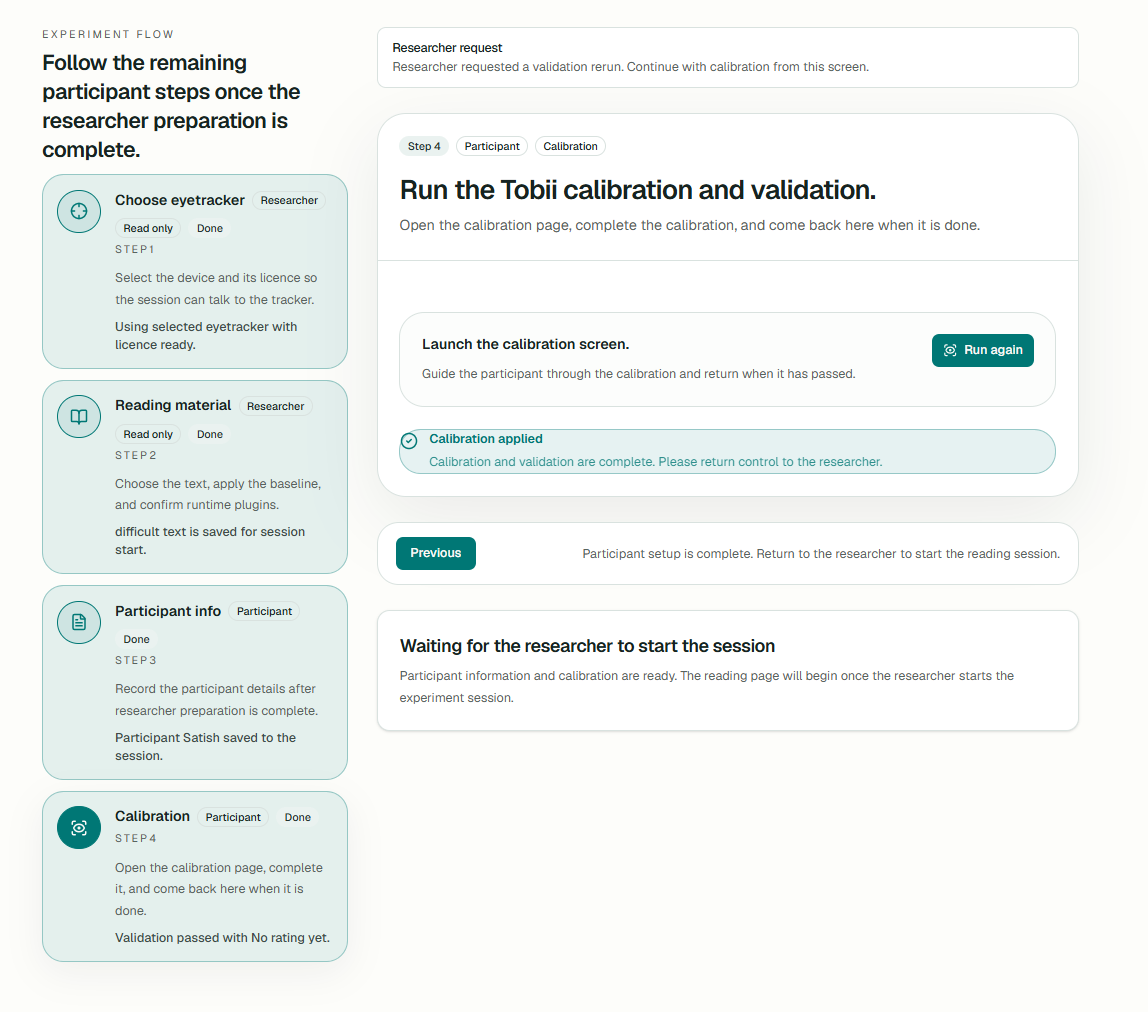
\includegraphics[width=\linewidth,height=0.86\textheight,keepaspectratio]{Backmatter/UserGuideImages/ParticipantWaitingScreen.png}}{\guidescreenshotpending{Backmatter/UserGuideImages/ParticipantWaitingScreen.png}}
  \caption{The participant waiting screen shown once setup is complete, before the session starts.}
  \end{figure}

  The reading page begins automatically when the researcher starts the session.
\end{itemize}

\begin{quote}
\textbf{Re-run calibration:} If the researcher requests a calibration or validation re-run, the
participant sees a notice and is routed back into calibration.
\end{quote}

\subsection{Calibration}\label{55-calibration}

Calibration maps the participant's gaze to the screen and then \textbf{validates} the result against a
quality threshold. It runs in \textbf{full screen} and must stay visible --- leaving full screen or hiding
the tab interrupts the run.

\begin{enumerate}
\def\labelenumi{\arabic{enumi}.}
\item
  On the \textbf{Ready} screen, the participant looks at the center of each target. A gaze-preview
  overlay helps confirm tracking. Click \textbf{Start}.

\begin{figure}[htbp]
  \centering
\IfFileExists{Backmatter/UserGuideImages/CalibrationReadyScreen.png}{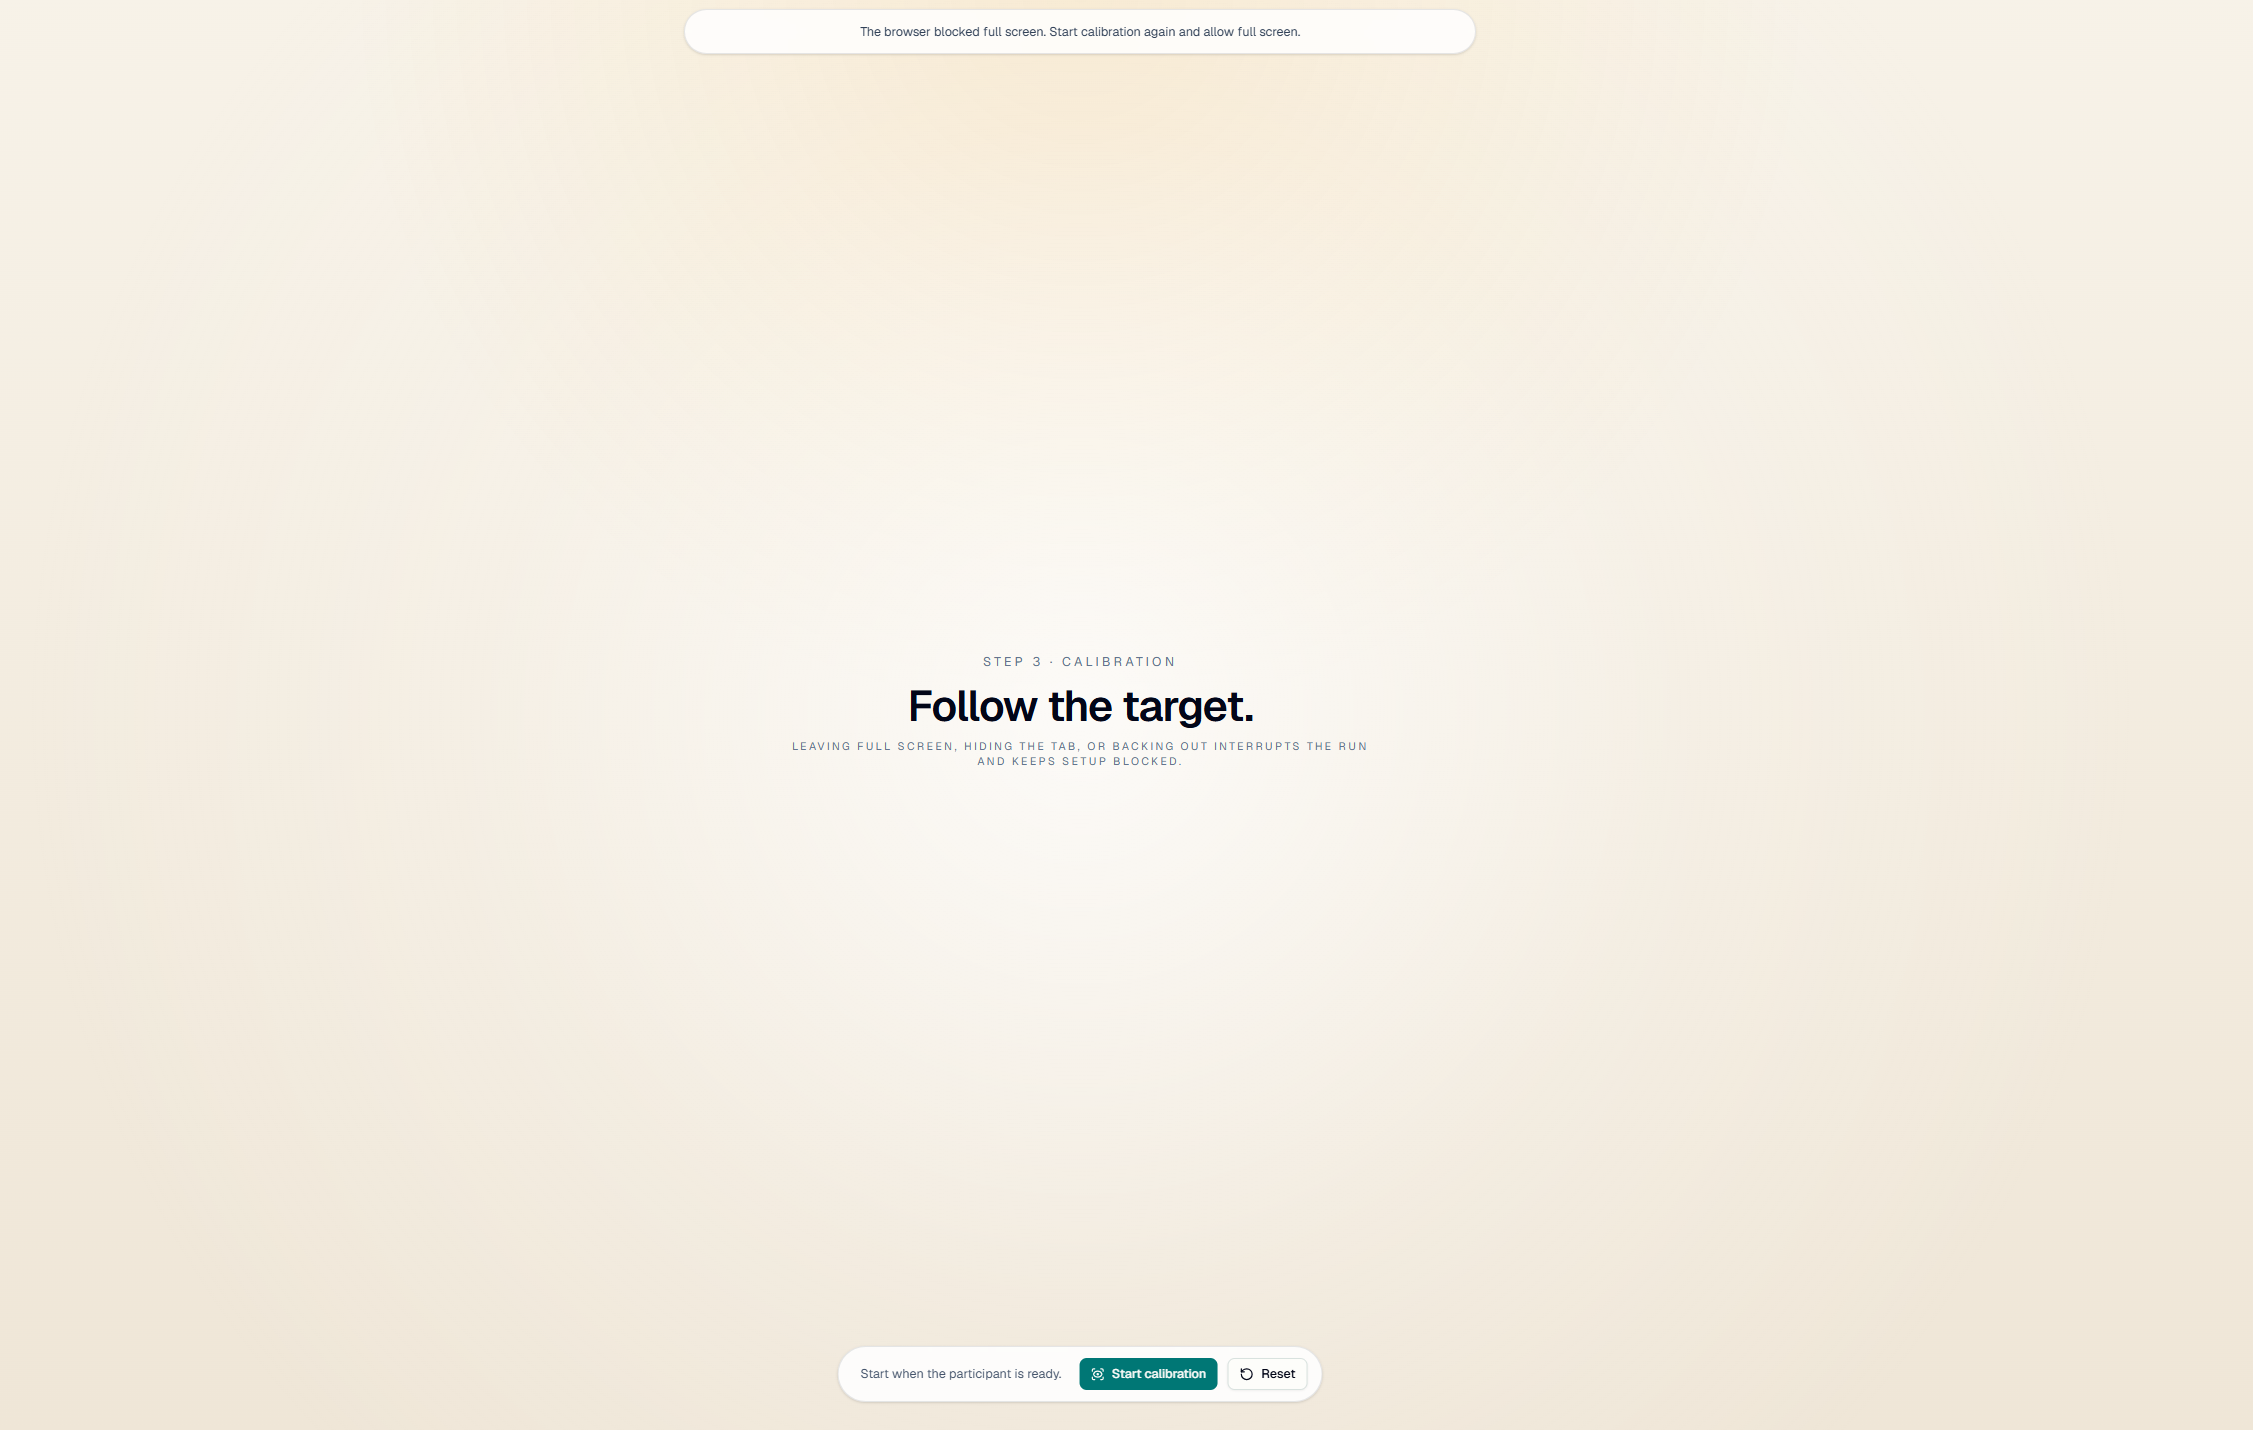
\includegraphics[width=\linewidth,height=0.86\textheight,keepaspectratio]{Backmatter/UserGuideImages/CalibrationReadyScreen.png}}{\guidescreenshotpending{Backmatter/UserGuideImages/CalibrationReadyScreen.png}}
  \caption{The calibration ready screen with the gaze-preview overlay.}
  \end{figure}
\item
  \textbf{Calibration run} --- a target moves point-to-point; the participant holds their gaze on each.

\begin{figure}[htbp]
  \centering
\IfFileExists{Backmatter/UserGuideImages/Calibration.png}{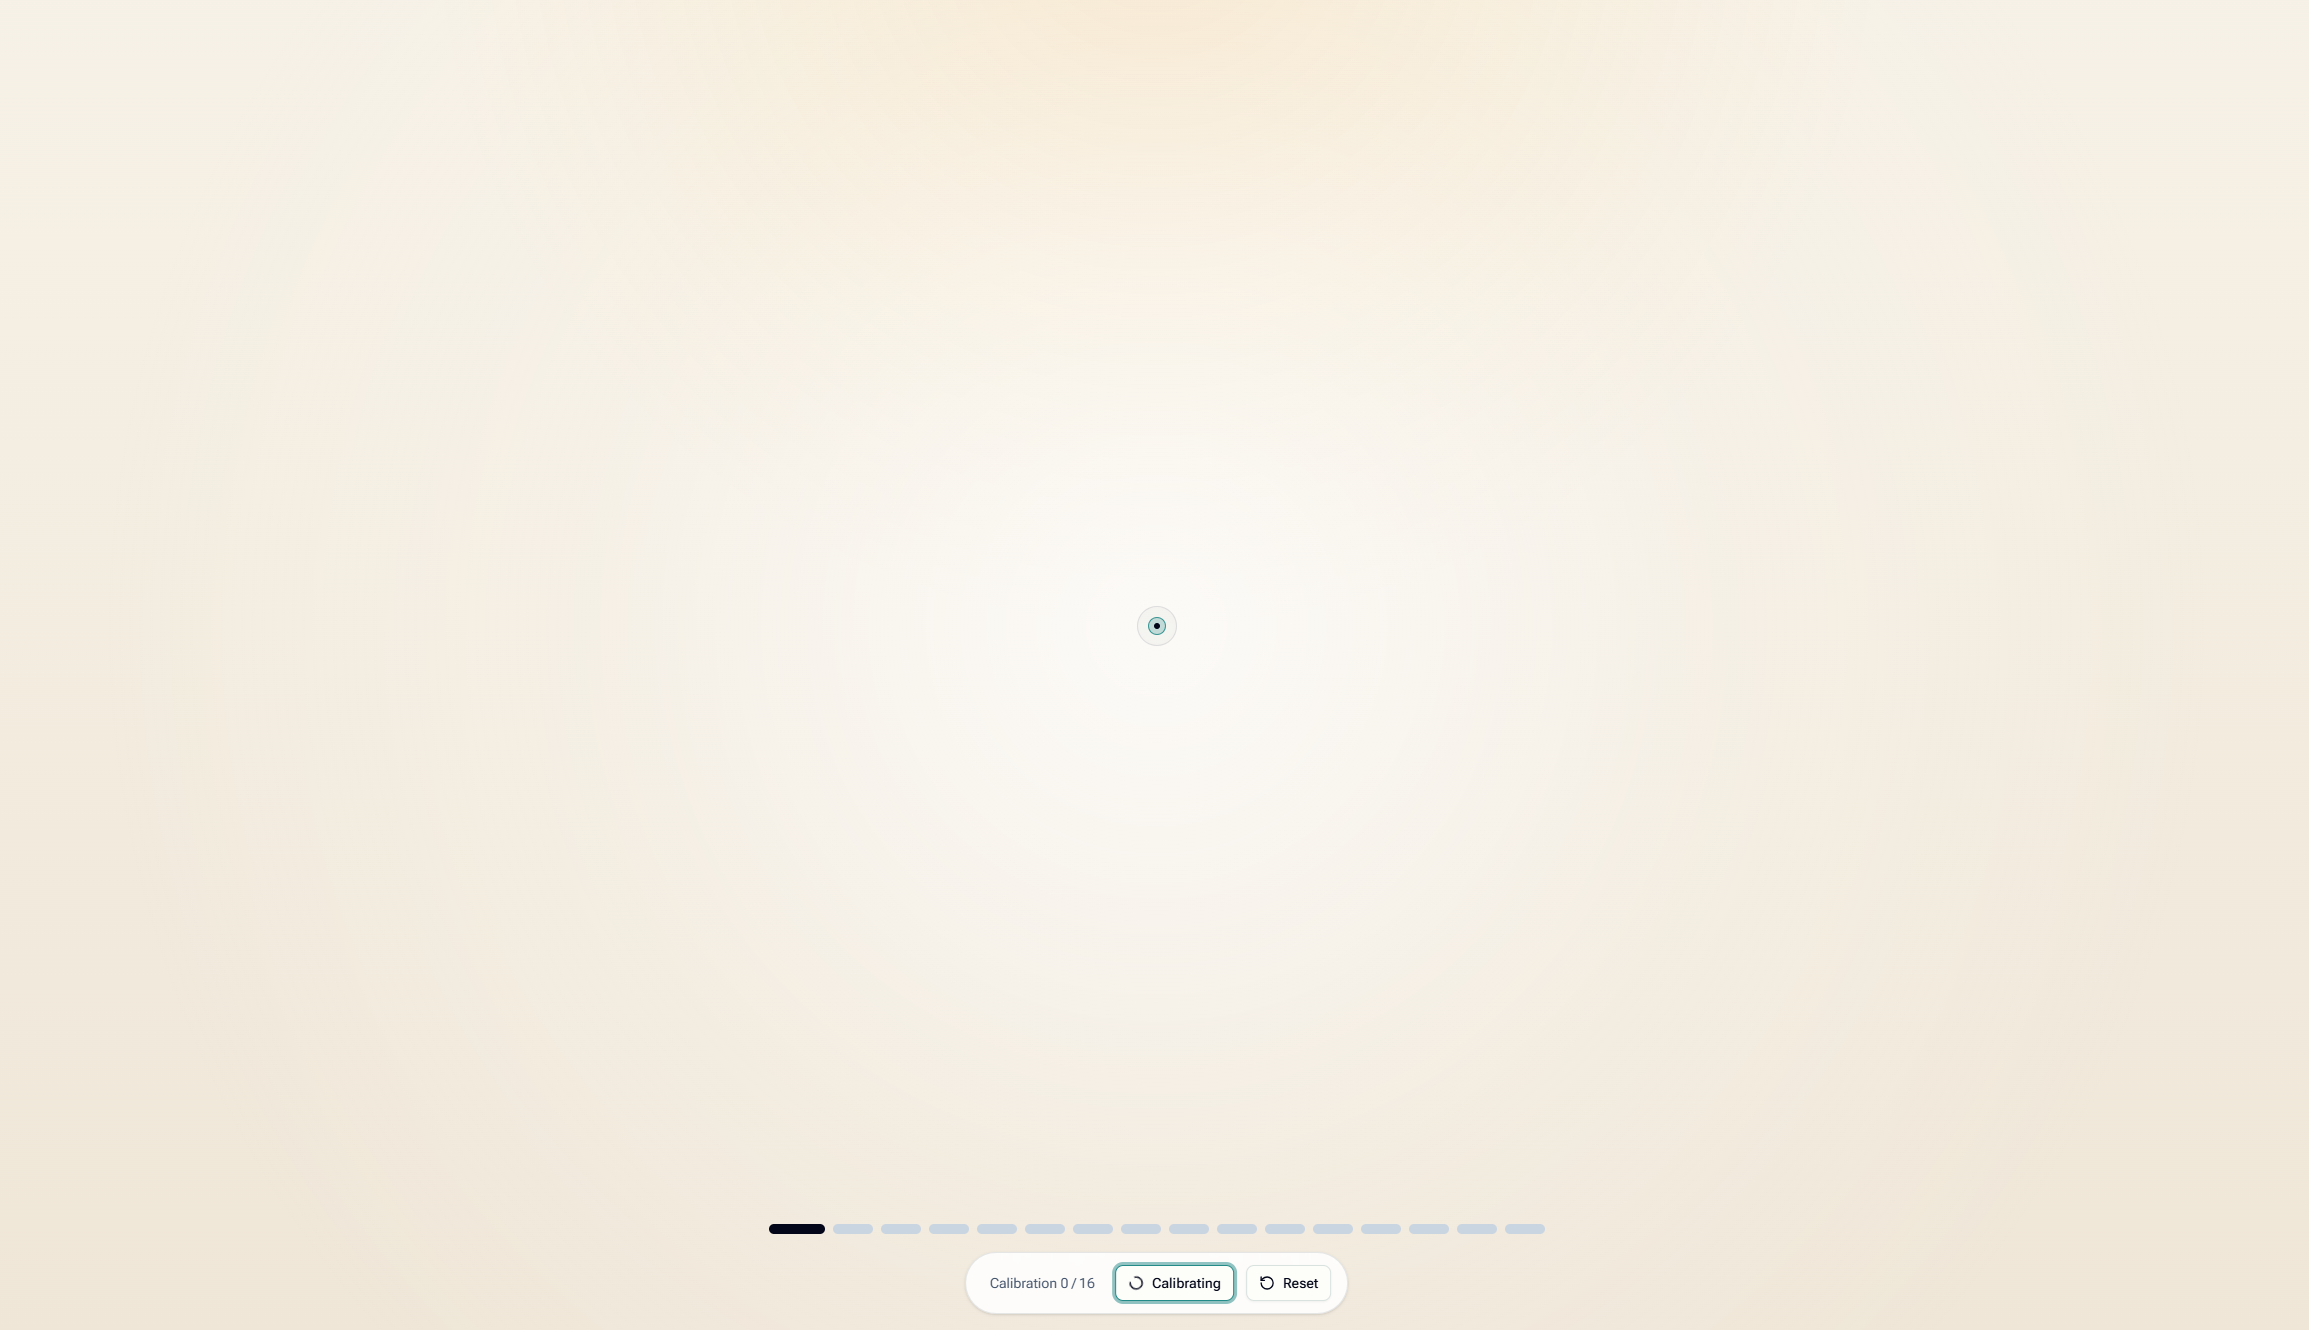
\includegraphics[width=\linewidth,height=0.86\textheight,keepaspectratio]{Backmatter/UserGuideImages/Calibration.png}}{\guidescreenshotpending{Backmatter/UserGuideImages/Calibration.png}}
  \caption{A calibration run in progress: the participant follows the moving target while the progress dots track collected points.}
  \end{figure}
\item
  \textbf{Validation run} --- repeats with validation targets to measure \textbf{accuracy} and \textbf{precision}.
\item
  \textbf{Review} \emph{(researcher mode)} --- shows quality, average accuracy/precision, and sample count.

  \begin{itemize}
  \tightlist
  \item
    If it \textbf{passed}, accept and return to the workflow.
  \item
    If it \textbf{failed}, \textbf{Rerun validation} or \textbf{Start} a fresh calibration.
  \end{itemize}

\begin{figure}[htbp]
  \centering
\IfFileExists{Backmatter/UserGuideImages/CalibrationMetrics.png}{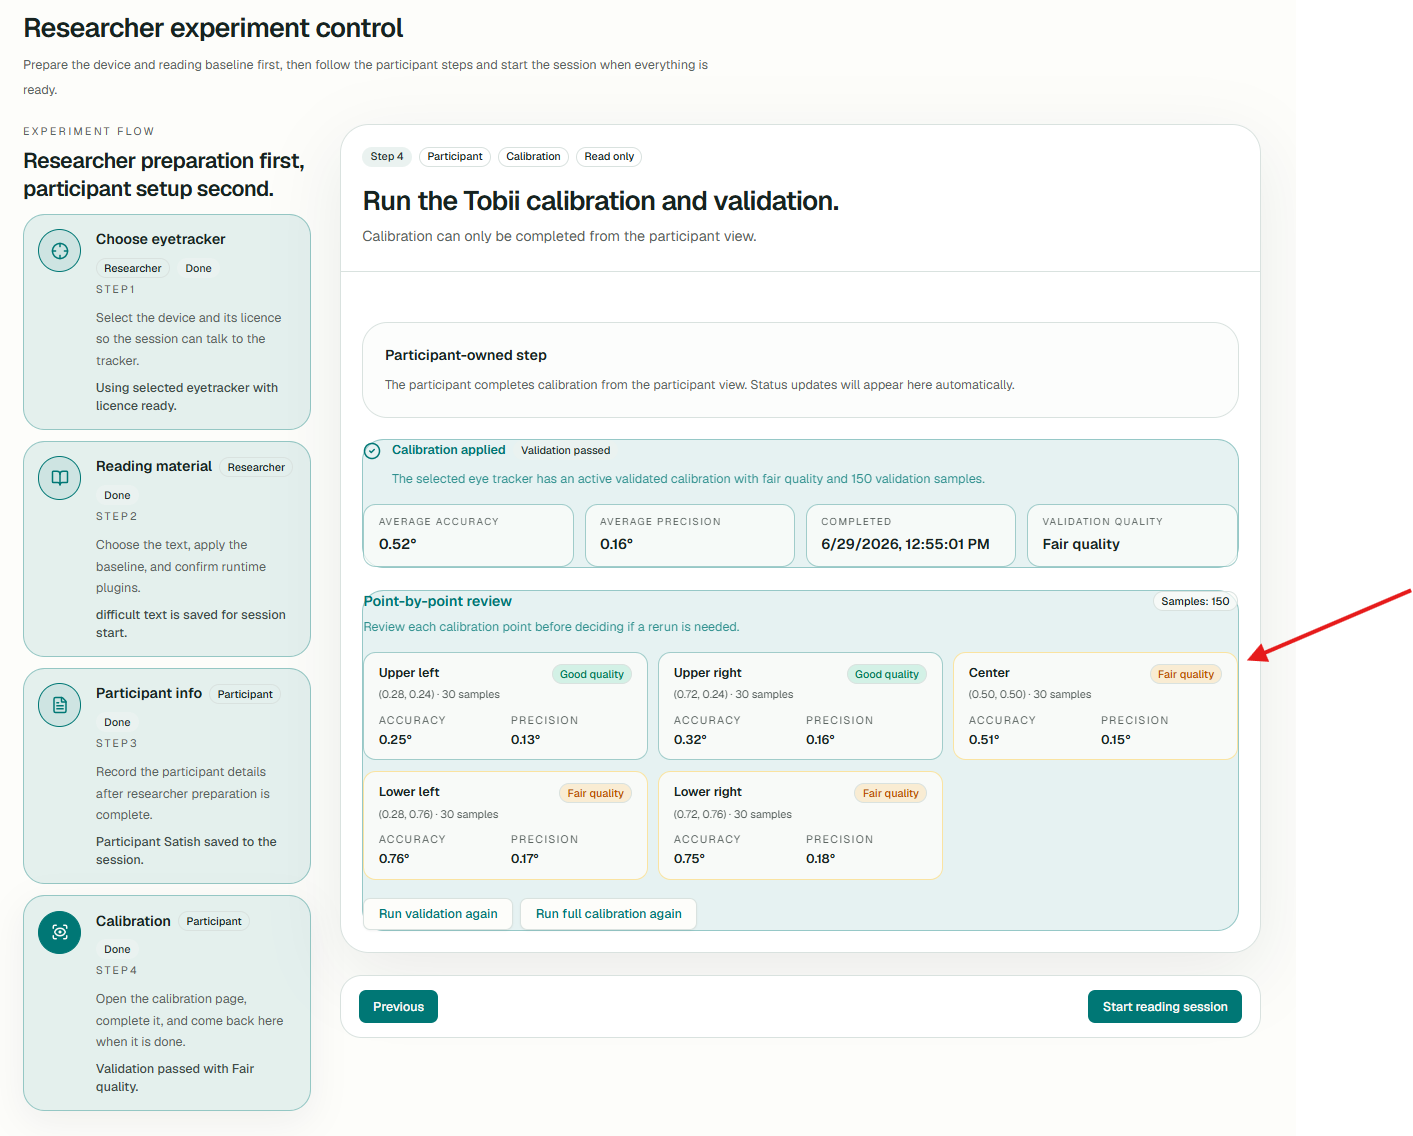
\includegraphics[width=\linewidth,height=0.86\textheight,keepaspectratio]{Backmatter/UserGuideImages/CalibrationMetrics.png}}{\guidescreenshotpending{Backmatter/UserGuideImages/CalibrationMetrics.png}}
  \caption{The calibration review panel showing quality, accuracy, and precision metrics.}
  \end{figure}
\item
  If a run is interrupted or rejected, a \textbf{failure} panel offers \textbf{Reset} or \textbf{Return to setup}.
\end{enumerate}

\begin{quote}
\textbf{Note:} In participant mode, a passing validation routes the participant straight back to their
setup; the metrics review is a researcher-mode step.
\end{quote}

\subsection{The Live Researcher View}\label{56-the-live-researcher-view}

Open \textbf{Researcher Live} to monitor the active session. It runs full screen and is laid out in
three columns.

\begin{figure}[htbp]
\centering
\IfFileExists{Backmatter/UserGuideImages/ResearcherLiveView.png}{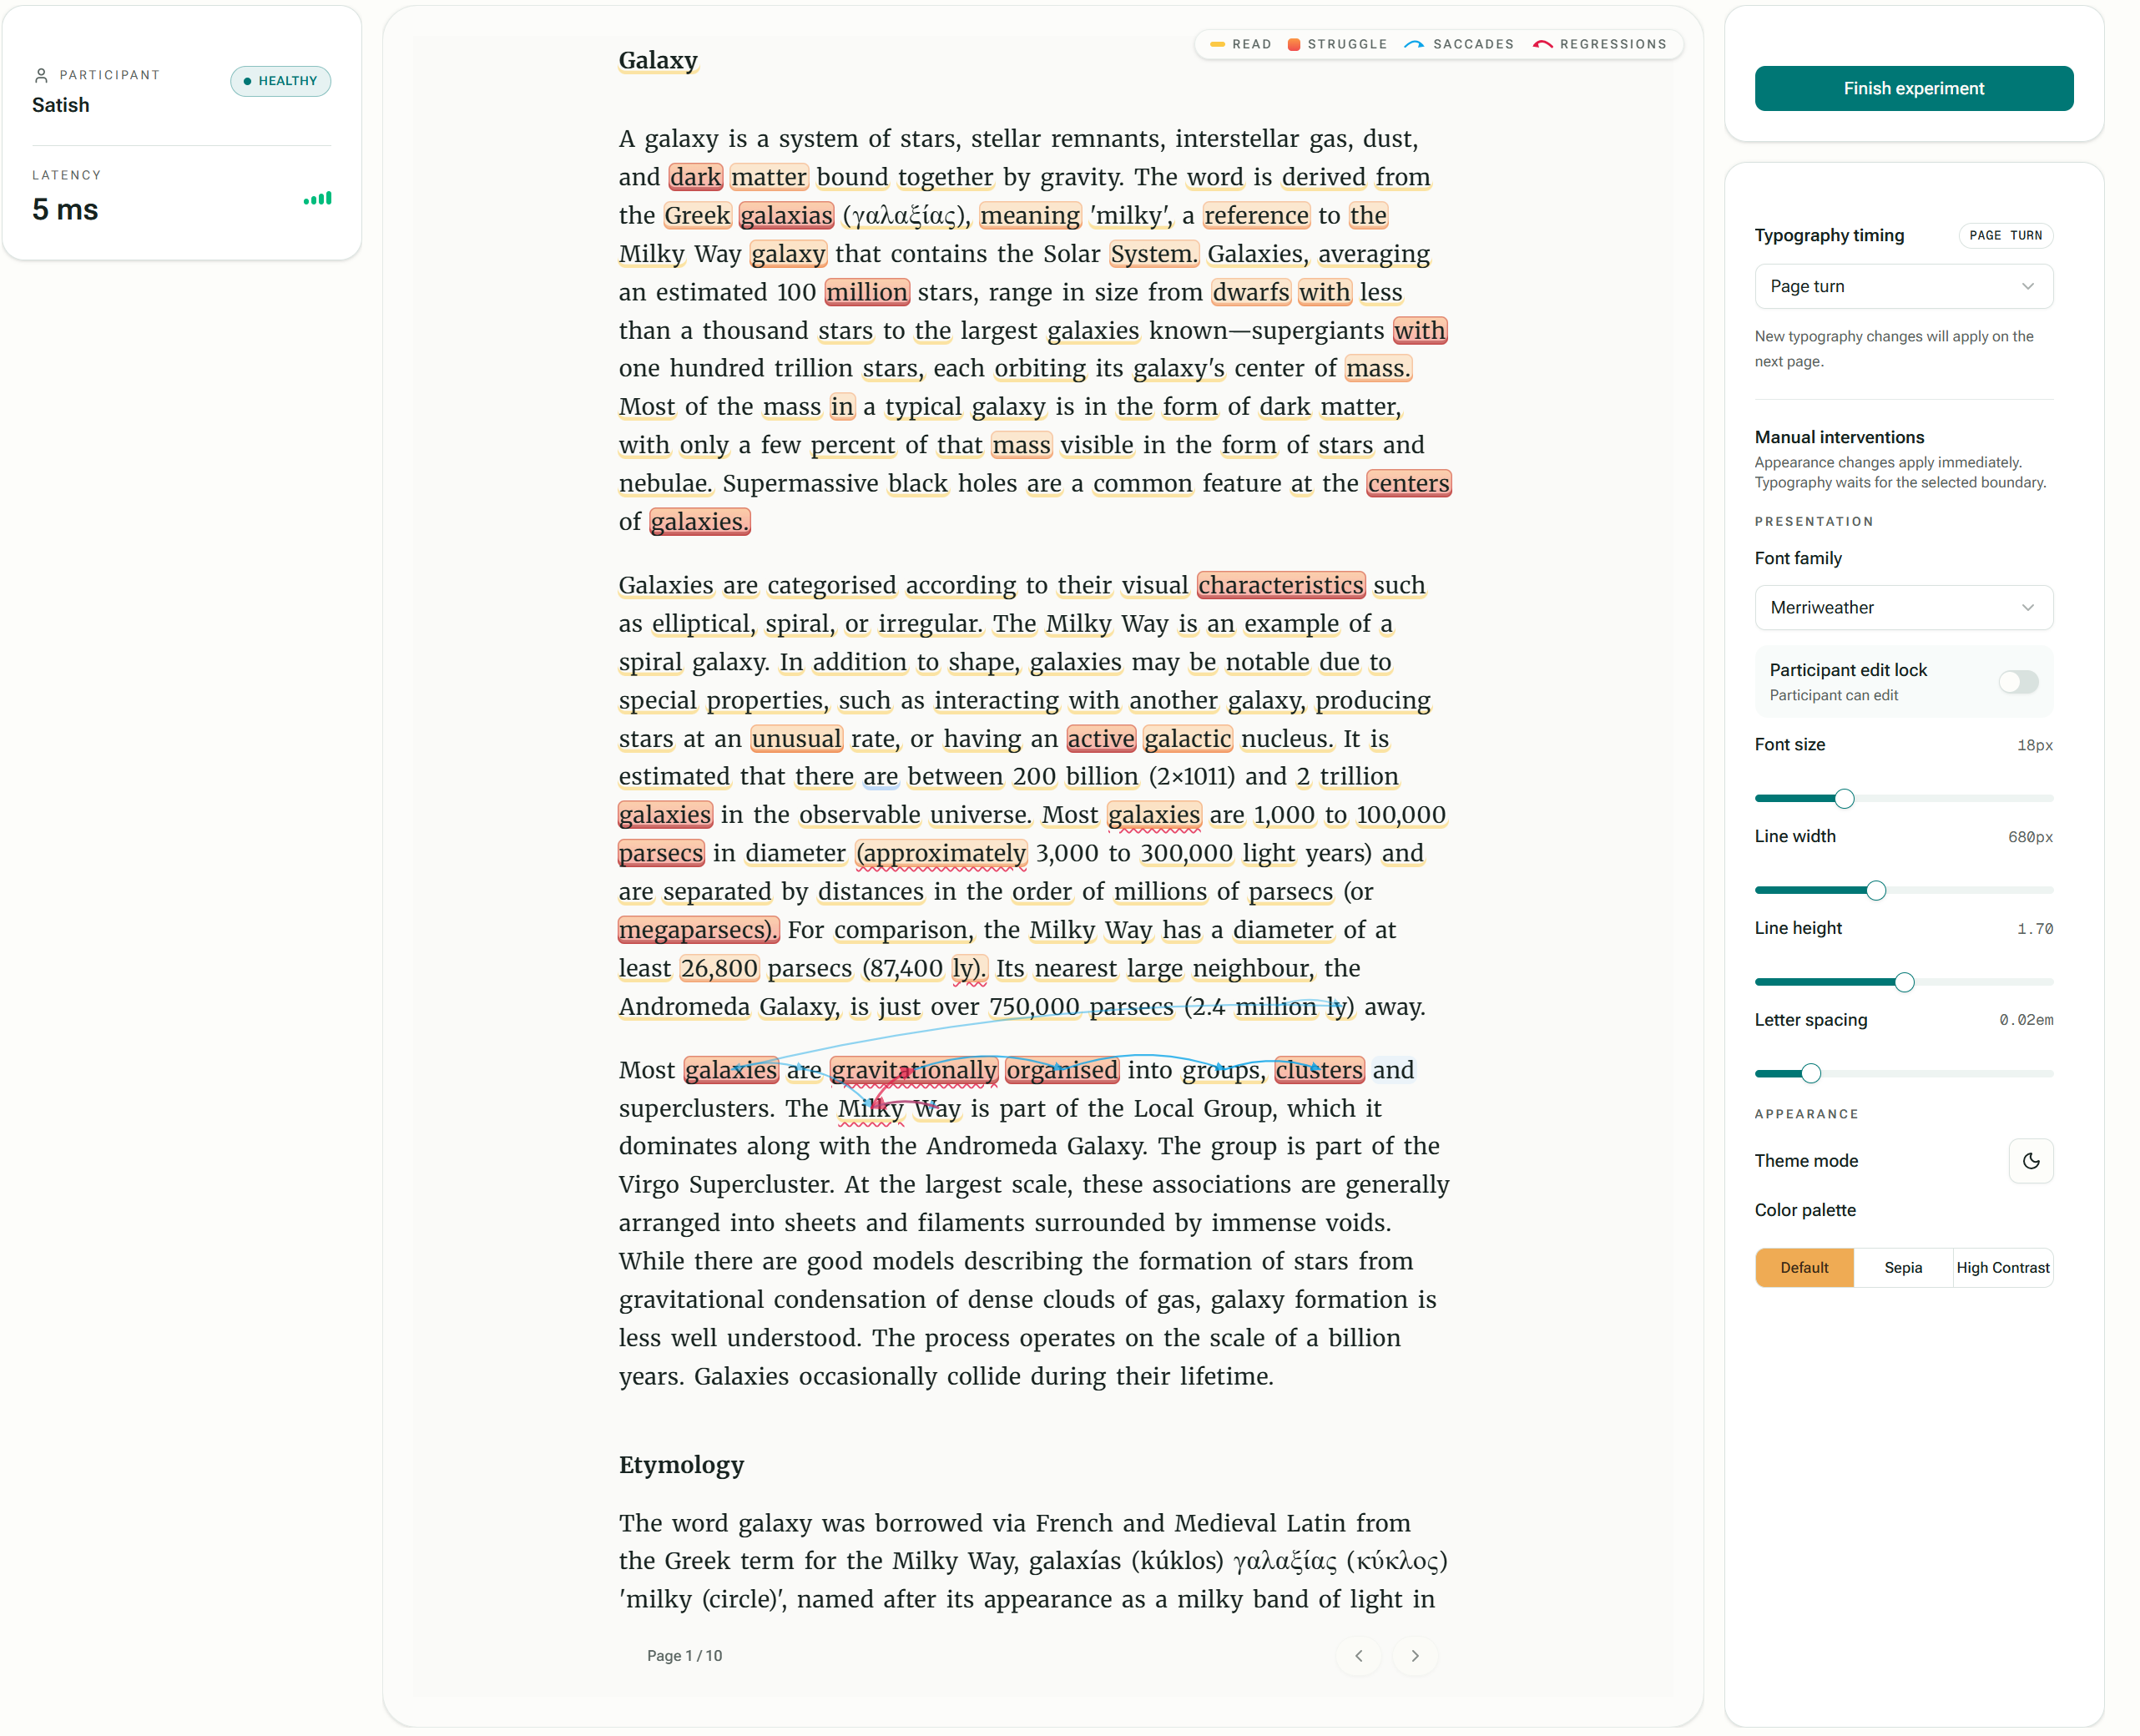
\includegraphics[width=\linewidth,height=0.86\textheight,keepaspectratio]{Backmatter/UserGuideImages/ResearcherLiveView.png}}{\guidescreenshotpending{Backmatter/UserGuideImages/ResearcherLiveView.png}}
\caption{The Researcher Live view: signals on the left, the live participant mirror in the center, and intervention controls on the right.}
\end{figure}

\textbf{Left column --- Live controls \& signals}
- Participant name and connection status.
- \textbf{Sample rate (Hz)}, \textbf{gaze validity rate}, and \textbf{latency (ms)}.
- \textbf{Struggle signals} (when the external eye analyzer is connected and selected).

\textbf{Center column --- Live reader (mirror)}
- A real-time mirror of what the participant sees, with their gaze focus highlighted.
- \textbf{Follow participant} keeps the mirror locked to the participant's scroll position.
- A trust banner appears when the mirror is only \emph{approximate} (e.g.~not full screen) --- click
\textbf{Enter full screen} to restore an exact mirror.
- Optional overlays (fixation heatmap, saccade path / ``reading dynamics'') via the reader controls.

\textbf{Right column --- Interventions}
- \textbf{Trigger an intervention} manually from the available intervention modules (e.g.~typography or
appearance changes), with a reason.
- \textbf{Approve / reject} decision proposals coming from a decision plugin (advisory mode).
- \textbf{Apply pending intervention now} to commit a queued change immediately.
- Set the \textbf{intervention commit boundary} (when a layout change is allowed to take effect).
- \textbf{Advance to the next text} in a multi-text experiment sequence.

\begin{figure}[htbp]
\centering
\IfFileExists{Backmatter/UserGuideImages/DesisionProvider.png}{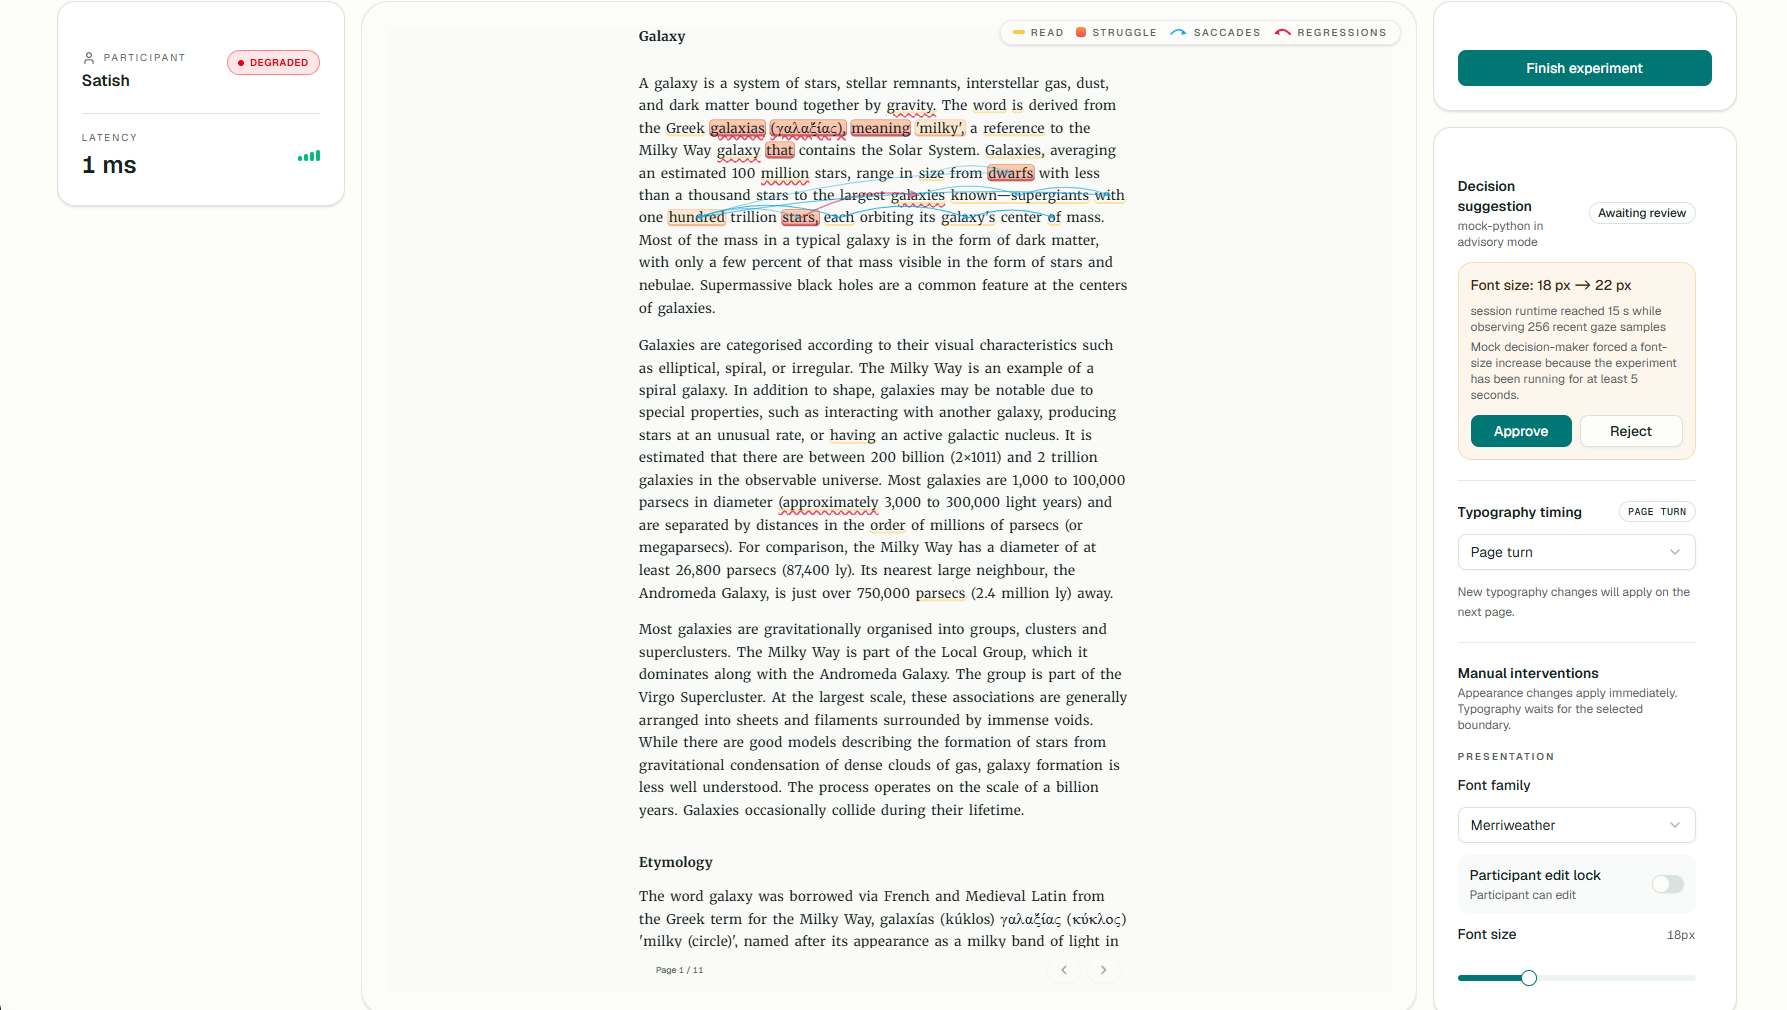
\includegraphics[width=\linewidth,height=0.86\textheight,keepaspectratio]{Backmatter/UserGuideImages/DesisionProvider.png}}{\guidescreenshotpending{Backmatter/UserGuideImages/DesisionProvider.png}}
\caption{The interventions column with the decision-provider proposal awaiting approval.}
\end{figure}

\subsection{Finishing \& Exporting a Session}\label{57-finishing--exporting-a-session}

When the session is finished:

\begin{enumerate}
\def\labelenumi{\arabic{enumi}.}
\item
  In the \textbf{Researcher Live} view (or its empty/complete state), click \textbf{Finish experiment}.

\begin{figure}[htbp]
  \centering
\IfFileExists{Backmatter/UserGuideImages/FInishButton.png}{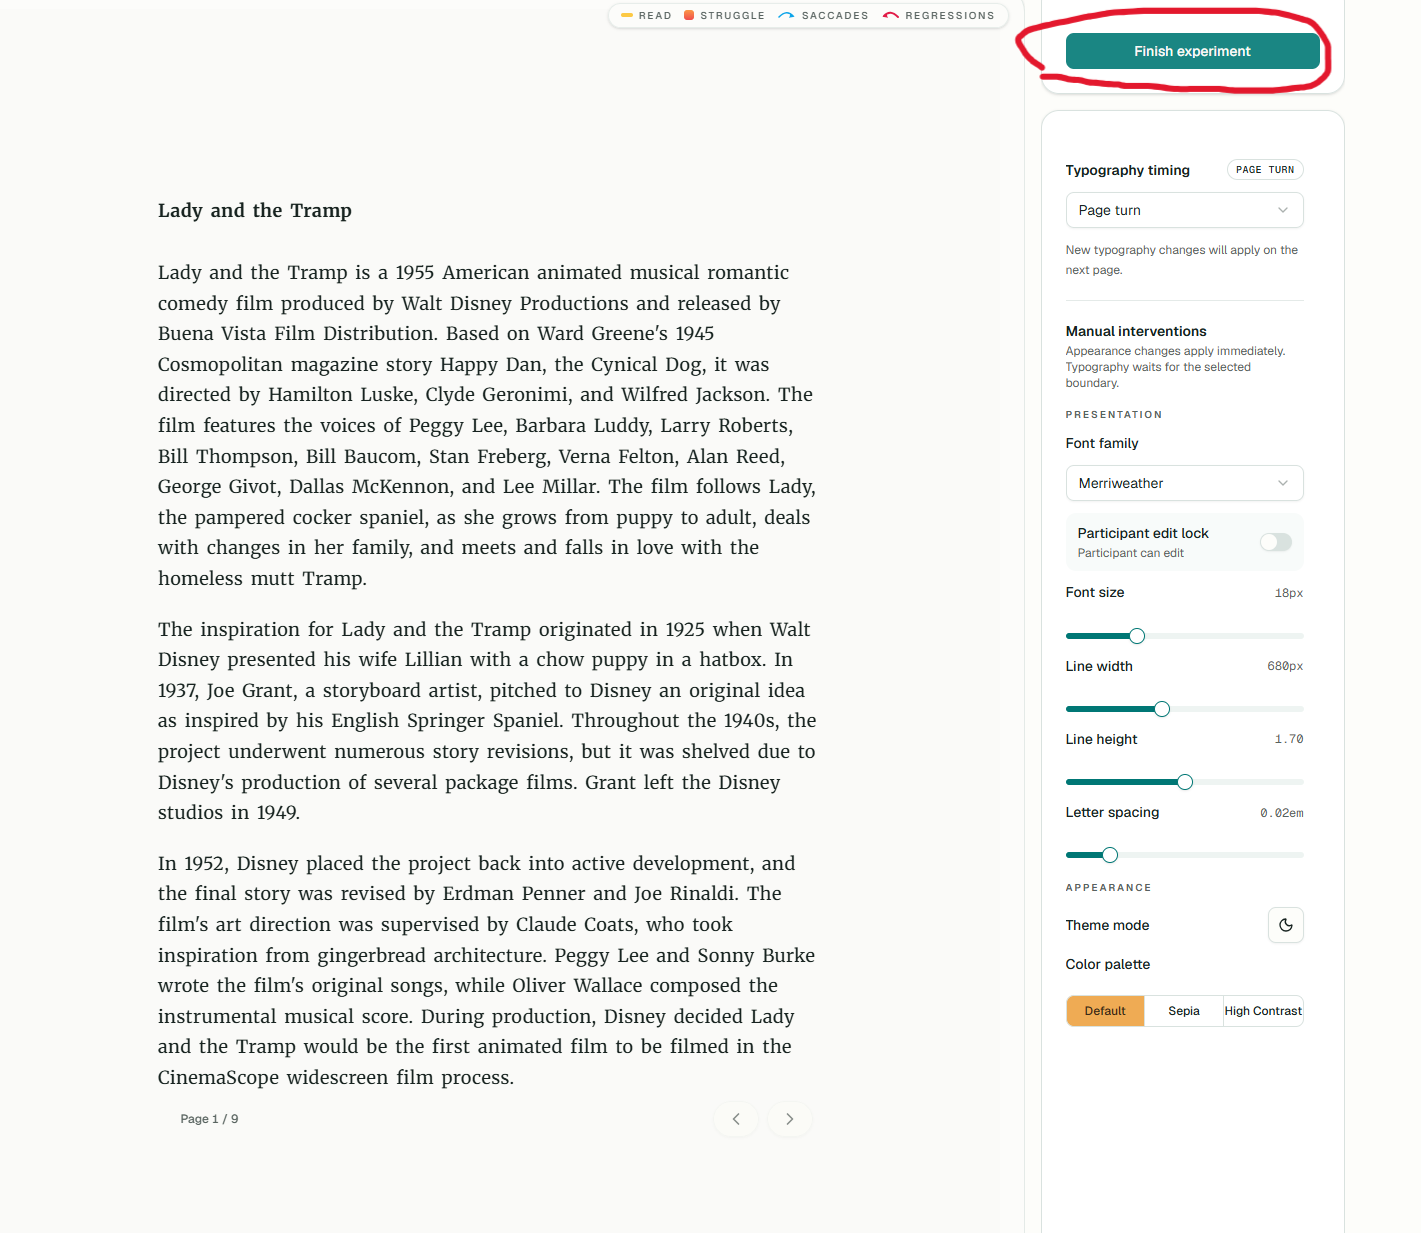
\includegraphics[width=\linewidth,height=0.86\textheight,keepaspectratio]{Backmatter/UserGuideImages/FInishButton.png}}{\guidescreenshotpending{Backmatter/UserGuideImages/FInishButton.png}}
  \caption{The Finish experiment button in the live view, used to end the session.}
  \end{figure}
\item
  After finishing, the completion actions appear. You can:

  \begin{itemize}
  \tightlist
  \item
    \textbf{Start new experiment} --- resets state and returns to the setup flow.
  \item
    \textbf{Download} the data as \textbf{JSON}, \textbf{CSV}, \textbf{Processed}, or \textbf{Telemetry}.
  \item
    \textbf{Save} the replay export (JSON or CSV) into the app under a name, so it appears in \textbf{Replay}.
  \end{itemize}

\begin{figure}[htbp]
  \centering
\IfFileExists{Backmatter/UserGuideImages/ExperimentFinished.png}{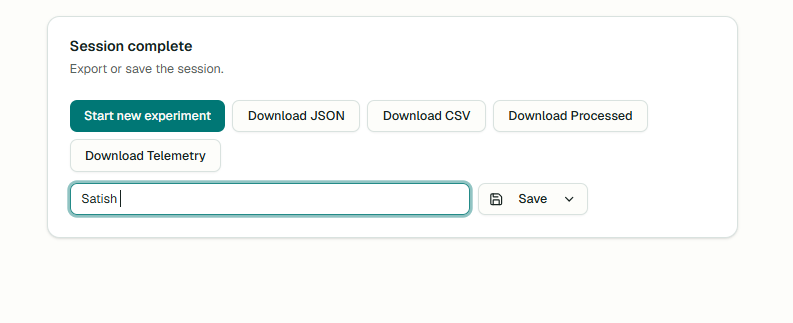
\includegraphics[width=\linewidth,height=0.86\textheight,keepaspectratio]{Backmatter/UserGuideImages/ExperimentFinished.png}}{\guidescreenshotpending{Backmatter/UserGuideImages/ExperimentFinished.png}}
  \caption{The session-complete card: export/download buttons and the export name + Save field.}
  \end{figure}
\end{enumerate}

\begin{quote}
\textbf{Naming:} The export name defaults to the reading title or participant name; edit it before
saving or downloading.
\end{quote}

\subsection{Replay a Saved Session}\label{58-replay-a-saved-session}

Open \textbf{Replay} to review a recorded session.

\begin{enumerate}
\def\labelenumi{\arabic{enumi}.}
\tightlist
\item
  \textbf{Load a session}:

  \begin{itemize}
  \tightlist
  \item
    Drag-and-drop or browse for an exported file, \textbf{or}
  \item
    Pick one of the \textbf{saved exports} listed on the upload screen.
  \item
    You can also \textbf{convert} a saved export into a processed report from here.
  \end{itemize}

\begin{figure}[htbp]
  \centering
\IfFileExists{Backmatter/UserGuideImages/ReplayFIle.png}{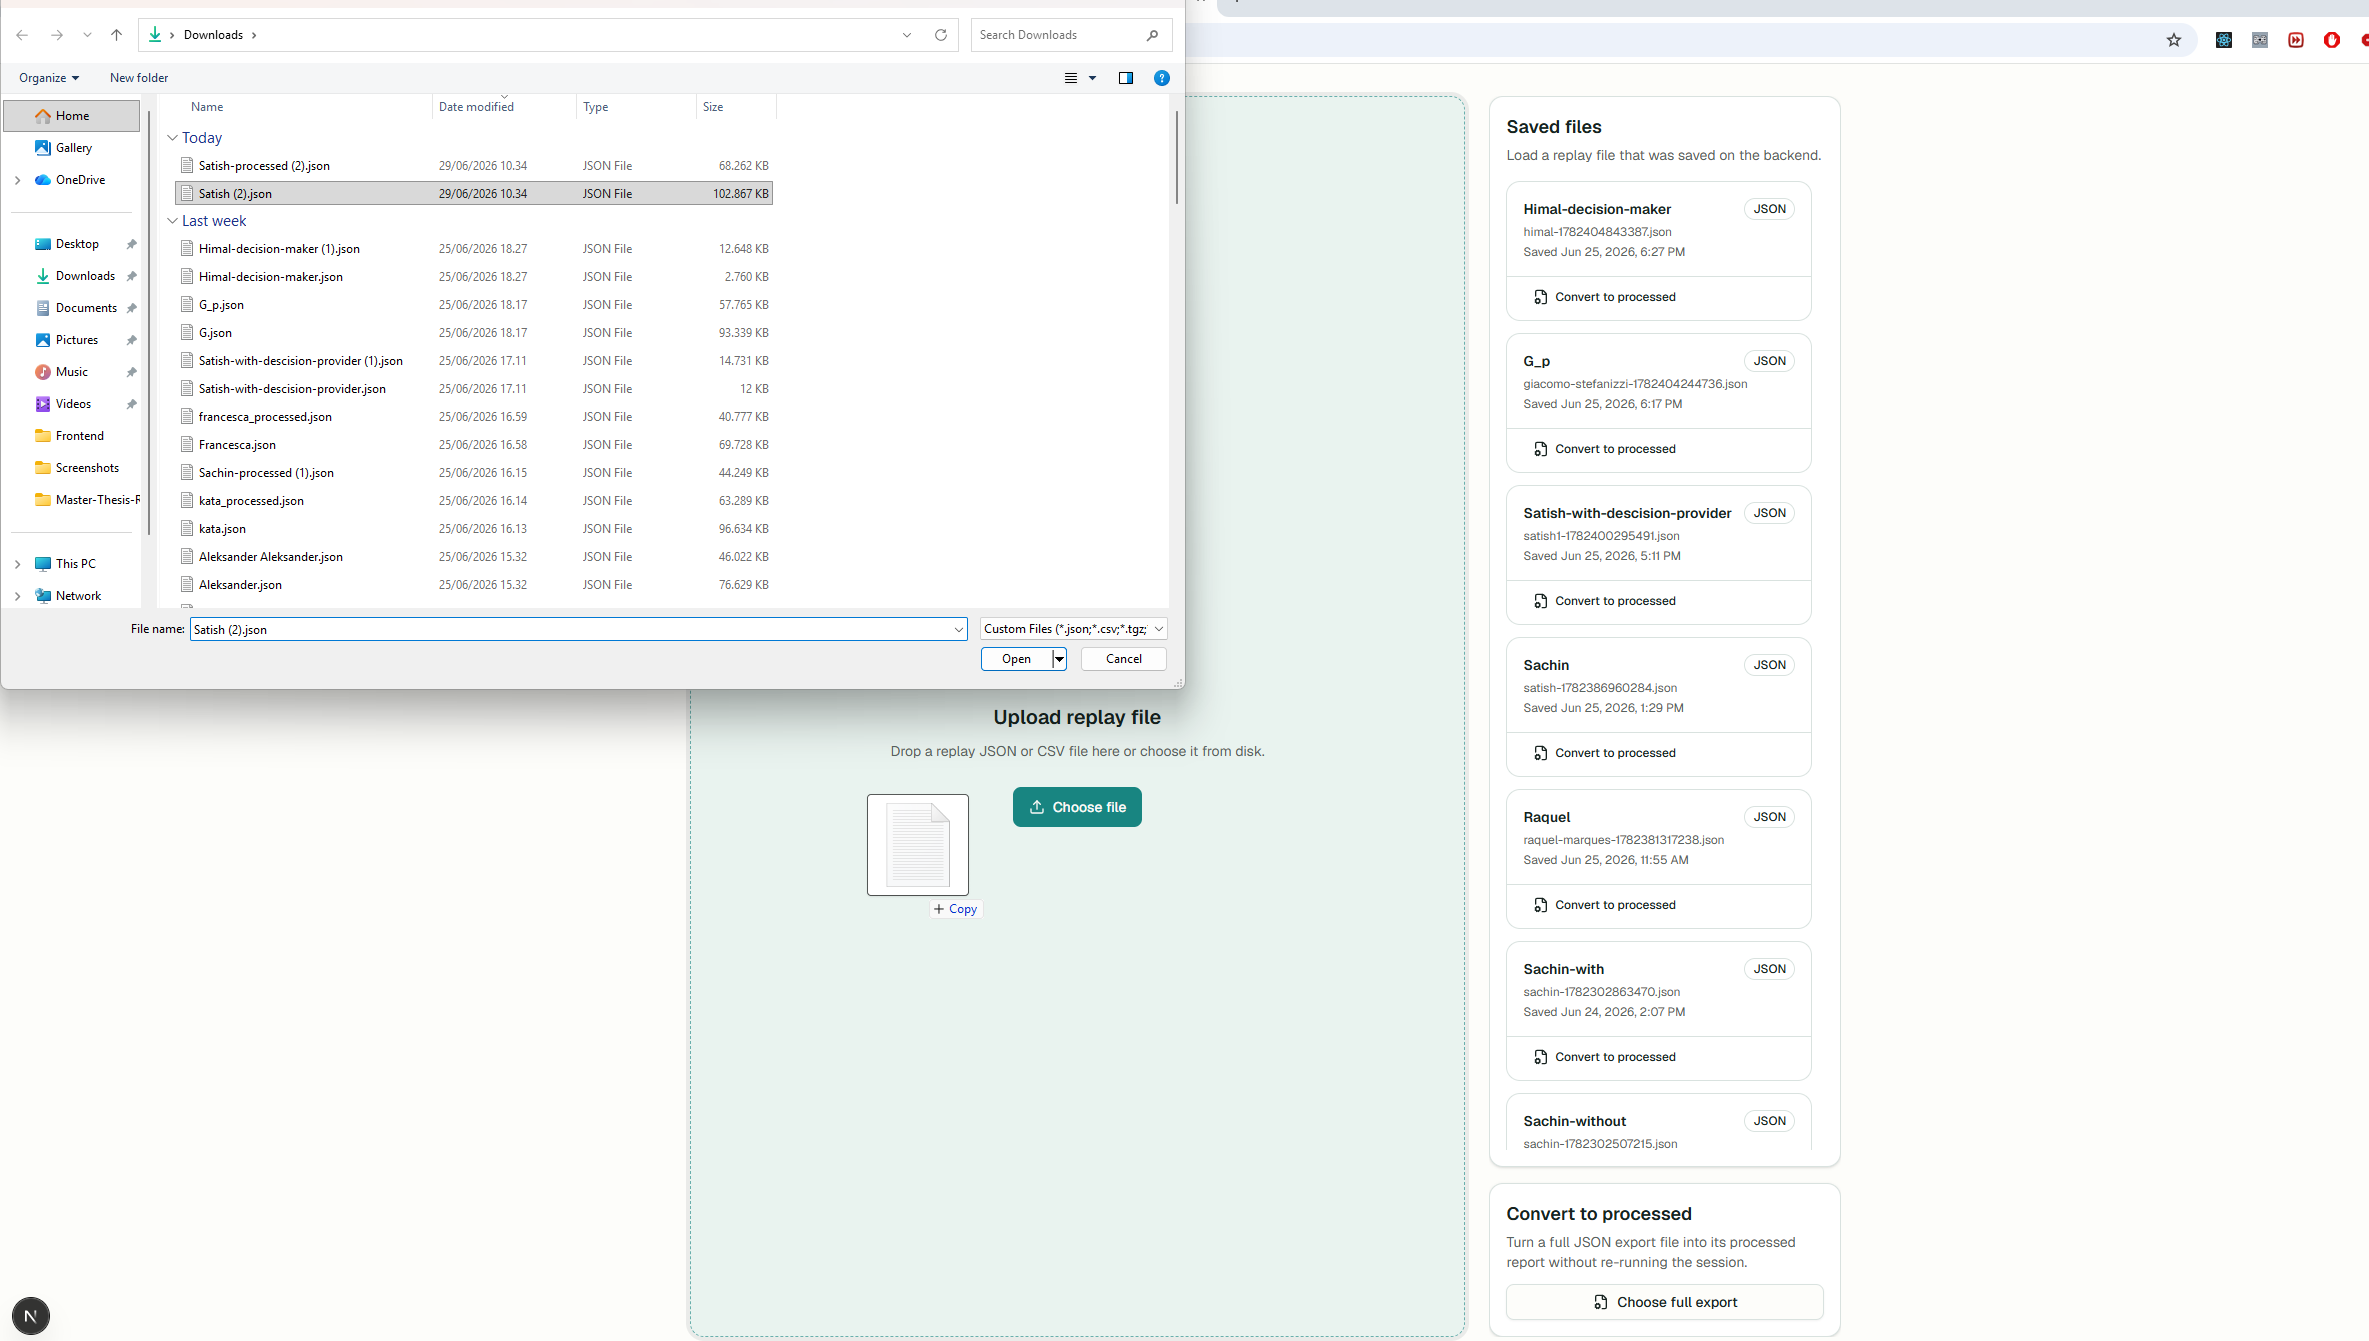
\includegraphics[width=\linewidth,height=0.86\textheight,keepaspectratio]{Backmatter/UserGuideImages/ReplayFIle.png}}{\guidescreenshotpending{Backmatter/UserGuideImages/ReplayFIle.png}}
  \caption{The replay upload screen: drag-and-drop area plus the list of saved exports.}
  \end{figure}
\item
  The replay opens in a three-column layout:

  \begin{itemize}
  \tightlist
  \item
    \textbf{Left} --- playback controls: play/pause, restart, scrubber, \textbf{playback speed}, reader
    overlay options, and load/clear.
  \item
    \textbf{Center} --- the reconstructed reading view at the current time, including gaze focus, saccade
    paths, and any quiz/finish screens that occurred.
  \item
    \textbf{Right} --- metadata and a \textbf{key-events timeline} (click an event to seek), plus oculomotor
    counts (\textbf{fixations, saccades, regressions}).
  \end{itemize}

\begin{figure}[htbp]
  \centering
\IfFileExists{Backmatter/UserGuideImages/Replay.png}{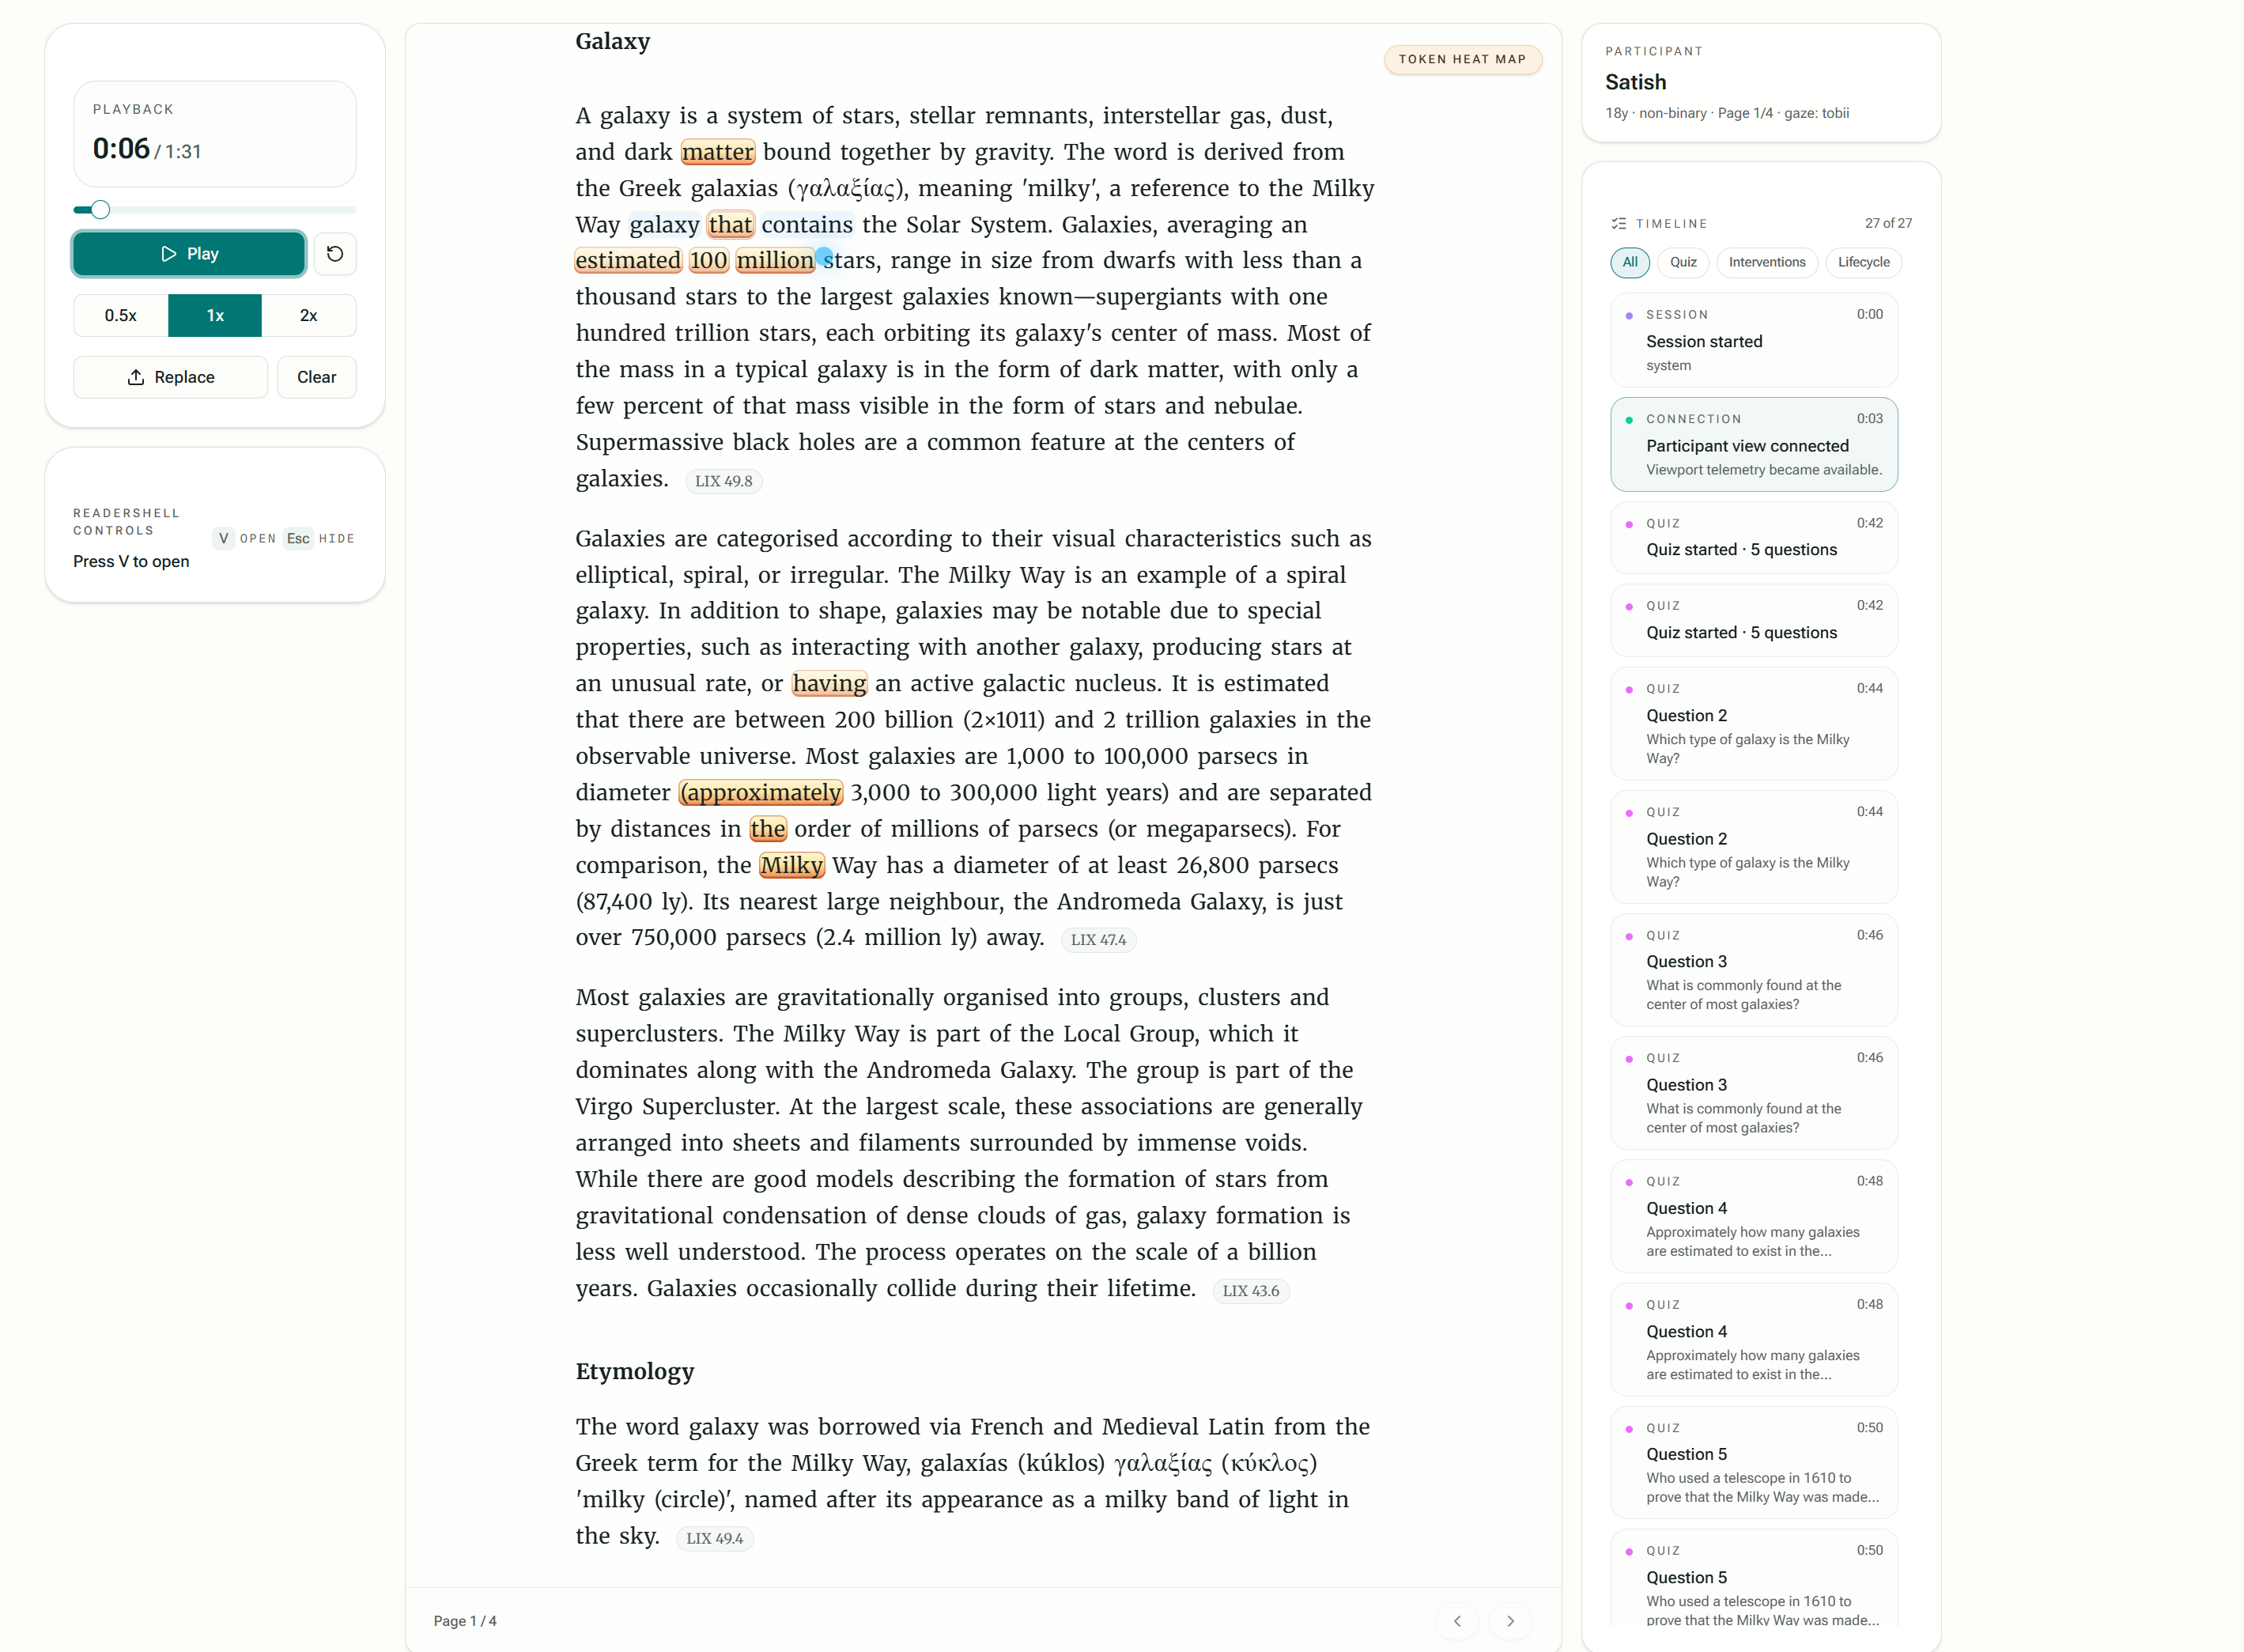
\includegraphics[width=\linewidth,height=0.86\textheight,keepaspectratio]{Backmatter/UserGuideImages/Replay.png}}{\guidescreenshotpending{Backmatter/UserGuideImages/Replay.png}}
  \caption{The replay player: playback controls on the left, the reconstructed reading view in the center, and the key-events timeline on the right.}
  \end{figure}
\end{enumerate}

\FloatBarrier
\section{Settings}\label{6-settings}

Open \textbf{Settings} from the sidebar. There are three sections (tabs):

\begin{figure}[htbp]
\centering
\IfFileExists{Backmatter/UserGuideImages/setingsPage.png}{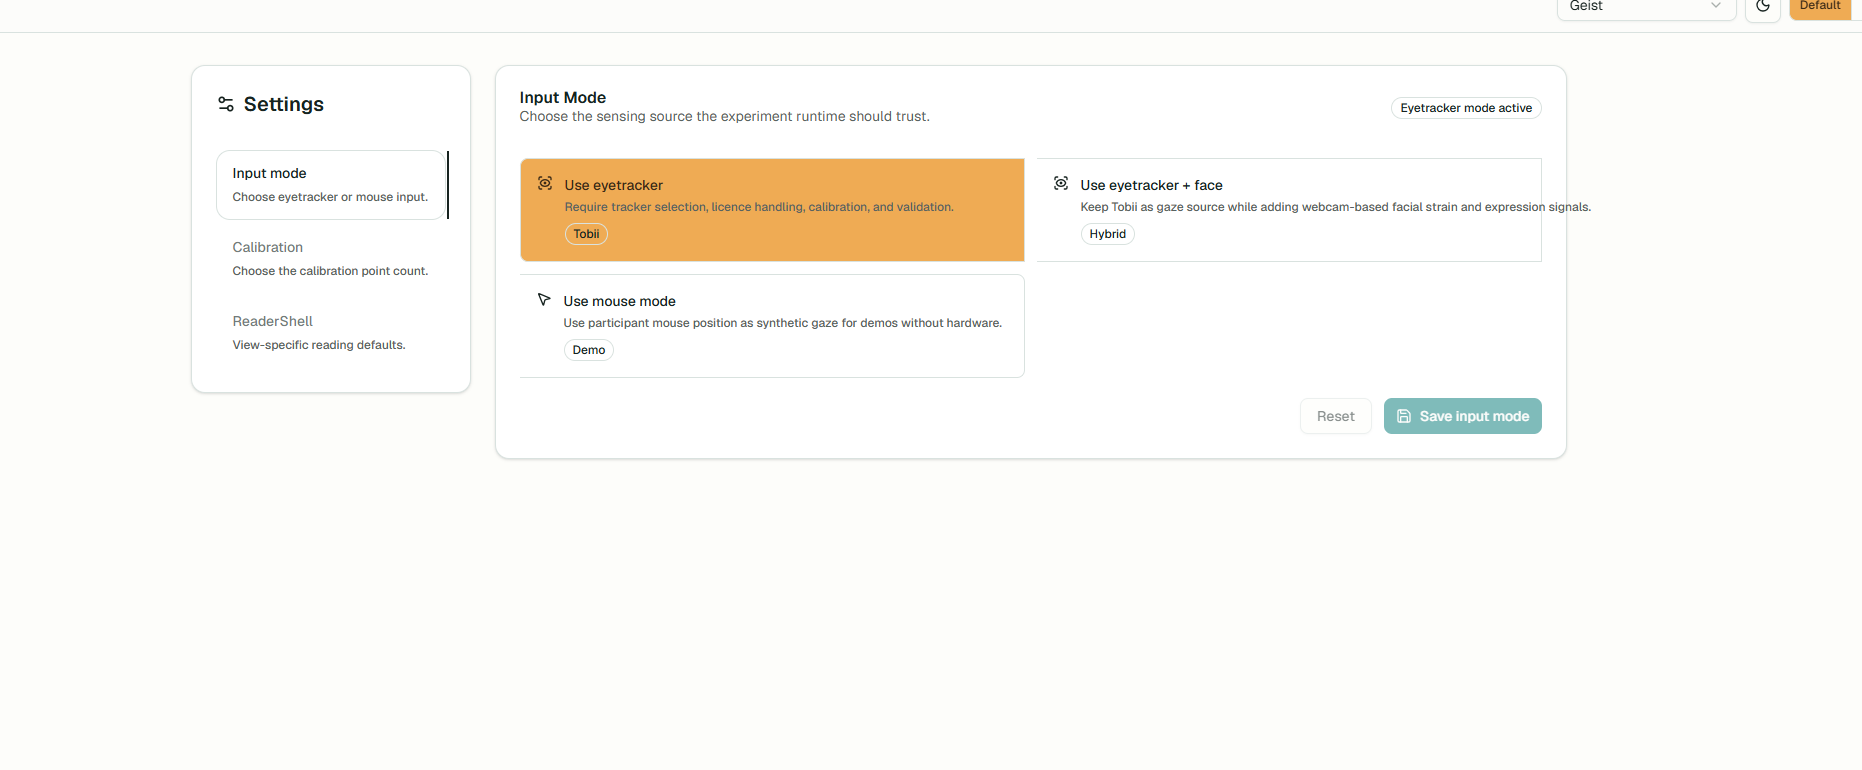
\includegraphics[width=\linewidth,height=0.86\textheight,keepaspectratio]{Backmatter/UserGuideImages/setingsPage.png}}{\guidescreenshotpending{Backmatter/UserGuideImages/setingsPage.png}}
\caption{The Settings page with its section tabs (Input mode, Calibration, ReaderShell).}
\end{figure}

{\small\def\LTcaptype{none} % do not increment counter
\begin{longtable}[]{@{}
  >{\raggedright\arraybackslash}p{(\linewidth - 2\tabcolsep) * \real{0.2500}}
  >{\raggedright\arraybackslash}p{(\linewidth - 2\tabcolsep) * \real{0.7500}}@{}}
\toprule\noalign{}
\begin{minipage}[b]{\linewidth}\raggedright
Section
\end{minipage} & \begin{minipage}[b]{\linewidth}\raggedright
What it controls
\end{minipage} \\
\midrule\noalign{}
\endhead
\bottomrule\noalign{}
\endlastfoot
\textbf{Input mode} & The sensing source: \textbf{Use eyetracker} (Tobii), \textbf{Use eyetracker + face} (Tobii gaze + webcam facial signals), or \textbf{Use mouse mode} (demo). Choose, then \textbf{Save}. See \cref{7-sensing-modes-explained}. \\
\textbf{Calibration} & The number of calibration points used during a calibration run. \\
\textbf{ReaderShell} & View-specific reading defaults for the researcher mirror and the replay reader (e.g.~which overlays are on by default). \\
\end{longtable}
}

\begin{quote}
The chosen input mode changes \textbf{Step 1} of the experiment stepper accordingly.
\end{quote}

\FloatBarrier
\section{Sensing Modes Explained}\label{7-sensing-modes-explained}

{\small\def\LTcaptype{none} % do not increment counter
\begin{longtable}[]{@{}
  >{\raggedright\arraybackslash}p{(\linewidth - 4\tabcolsep) * \real{0.2174}}
  >{\raggedright\arraybackslash}p{(\linewidth - 4\tabcolsep) * \real{0.1304}}
  >{\raggedright\arraybackslash}p{(\linewidth - 4\tabcolsep) * \real{0.6522}}@{}}
\toprule\noalign{}
\begin{minipage}[b]{\linewidth}\raggedright
Mode
\end{minipage} & \begin{minipage}[b]{\linewidth}\raggedright
Badge
\end{minipage} & \begin{minipage}[b]{\linewidth}\raggedright
Behavior
\end{minipage} \\
\midrule\noalign{}
\endhead
\bottomrule\noalign{}
\endlastfoot
\textbf{Use eyetracker} & Tobii & Requires tracker selection, licence handling, calibration, and validation. The standard real-experiment mode. \\
\textbf{Use eyetracker + face} & Hybrid & Tobii stays the authoritative gaze source; a webcam adds facial strain/expression signals. If the webcam is unavailable, gaze still runs but facial signals are degraded. \\
\textbf{Use mouse mode} & Demo & The participant's mouse position is used as synthetic gaze. Skips tracker selection, licence, and hardware checks --- ideal for demos without hardware. \\
\end{longtable}
}

\begin{figure}[htbp]
\centering
\IfFileExists{Backmatter/UserGuideImages/MouseMOdeSelected.png}{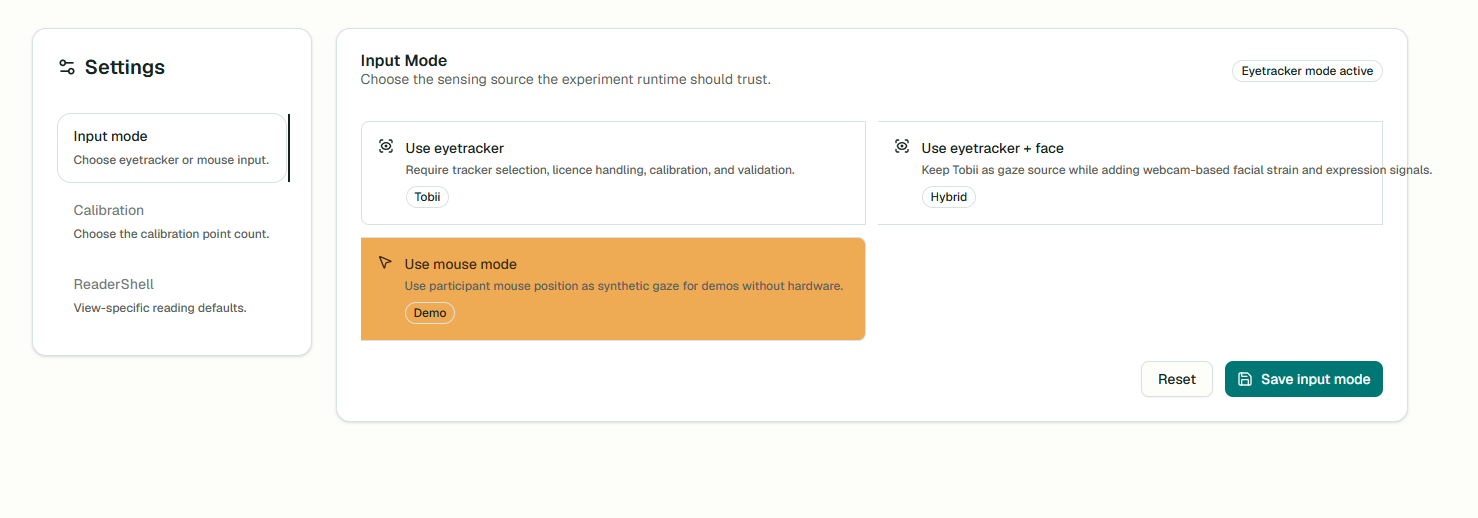
\includegraphics[width=\linewidth,height=0.86\textheight,keepaspectratio]{Backmatter/UserGuideImages/MouseMOdeSelected.png}}{\guidescreenshotpending{Backmatter/UserGuideImages/MouseMOdeSelected.png}}
\caption{Input mode selection with Use mouse mode chosen.}
\end{figure}

\FloatBarrier
\section{Runtime Plugins (Decision \& Eye Analysis)}\label{8-runtime-plugins-decision--eye-analysis}

The platform separates \textbf{who decides on interventions} from \textbf{who analyzes eye movement}. Both are
selectable per session in \textbf{Step 2}, and a default decision strategy is stored on each template.

\textbf{Decision plugin} options:

{\small\def\LTcaptype{none} % do not increment counter
\begin{longtable}[]{@{}
  >{\raggedright\arraybackslash}p{(\linewidth - 2\tabcolsep) * \real{0.2500}}
  >{\raggedright\arraybackslash}p{(\linewidth - 2\tabcolsep) * \real{0.7500}}@{}}
\toprule\noalign{}
\begin{minipage}[b]{\linewidth}\raggedright
Option
\end{minipage} & \begin{minipage}[b]{\linewidth}\raggedright
Meaning
\end{minipage} \\
\midrule\noalign{}
\endhead
\bottomrule\noalign{}
\endlastfoot
\textbf{Manual control} & Interventions stay fully researcher-operated. No decision plugin. \\
\textbf{Rule-based advisory} & Built-in rules \emph{propose} interventions for the researcher to approve. \\
\textbf{Rule-based autonomous} & Built-in rules \emph{apply} supported interventions automatically. \\
\textbf{Decision-maker advisory} & A connected external service proposes interventions. \\
\textbf{Decision-maker autonomous} & A connected external service requests interventions automatically. \\
\end{longtable}
}

\textbf{Eye analyzer} options:

{\small\def\LTcaptype{none} % do not increment counter
\begin{longtable}[]{@{}
  >{\raggedright\arraybackslash}p{(\linewidth - 2\tabcolsep) * \real{0.2500}}
  >{\raggedright\arraybackslash}p{(\linewidth - 2\tabcolsep) * \real{0.7500}}@{}}
\toprule\noalign{}
\begin{minipage}[b]{\linewidth}\raggedright
Option
\end{minipage} & \begin{minipage}[b]{\linewidth}\raggedright
Meaning
\end{minipage} \\
\midrule\noalign{}
\endhead
\bottomrule\noalign{}
\endlastfoot
\textbf{Built-in analyzer} & Backend thresholds provide fixation/saccade state. \\
\textbf{Eye analyzer service} & A connected external service supplies fixation/saccade and struggle state. \\
\end{longtable}
}

\begin{quote}
External options are only selectable when the corresponding service is \textbf{connected} and supports
the chosen mode. Otherwise the option shows \textbf{--- unavailable} and the built-in option remains
active.
\end{quote}

\begin{figure}[htbp]
\centering
\IfFileExists{Backmatter/UserGuideImages/Plugins.png}{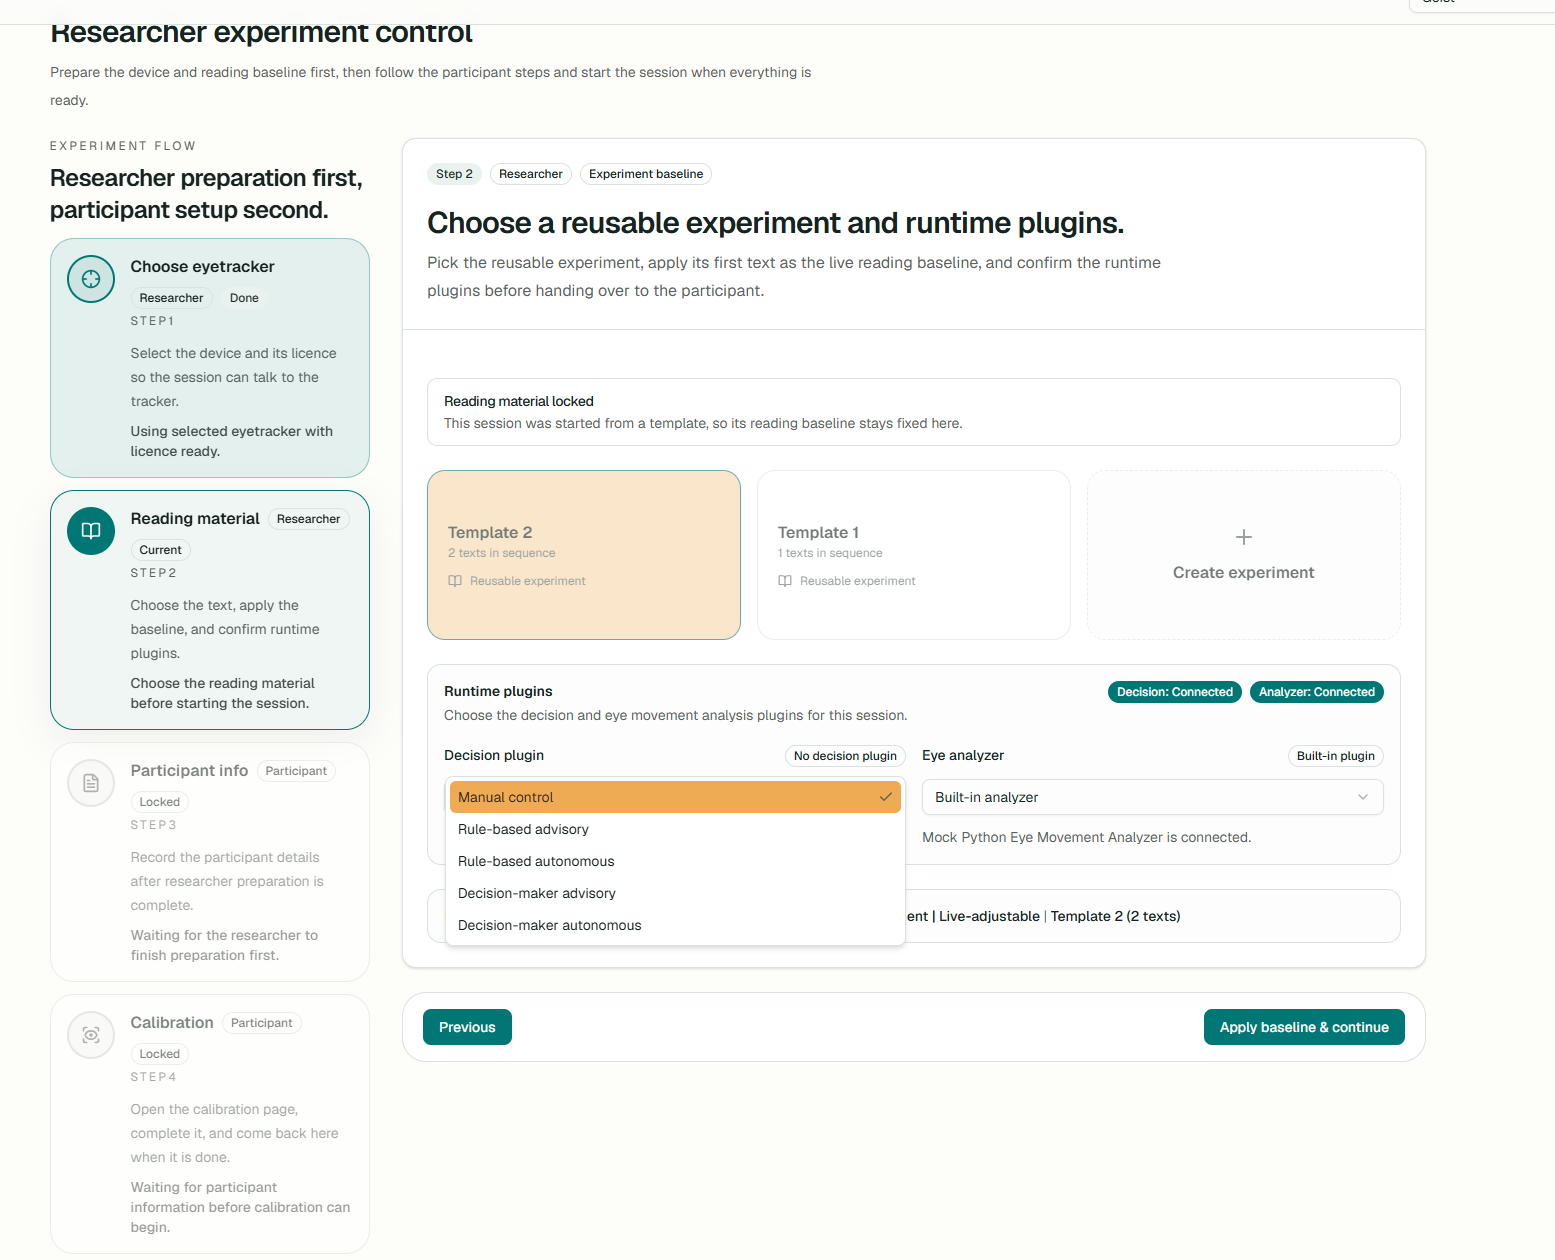
\includegraphics[width=\linewidth,height=0.86\textheight,keepaspectratio]{Backmatter/UserGuideImages/Plugins.png}}{\guidescreenshotpending{Backmatter/UserGuideImages/Plugins.png}}
\caption{The runtime plugin selectors (decision plugin and eye analyzer) with their status badges.}
\end{figure}

\FloatBarrier
\section{Troubleshooting \& FAQ}\label{9-troubleshooting--faq}

\textbf{The participant page is stuck on ``waiting''.}
The researcher hasn't finished Steps 1--2 yet, or the session hasn't started. Complete researcher
preparation; the participant steps unlock automatically.

\textbf{Calibration keeps getting interrupted.}
Calibration must stay in \textbf{full screen} and remain the visible tab for the whole run. If the
browser blocks full screen, start again and allow it. Don't switch tabs or windows during the run.

\textbf{An external decision/analyzer option says ``unavailable''.}
The external service isn't connected (or doesn't support that mode). Reconnect the service, or pick
a built-in option.

\textbf{The live mirror shows an ``approximate'' banner.}
The researcher view isn't in full screen, or participant viewport data is missing. Click \textbf{Enter
full screen} to restore an exact mirror.

\textbf{I can't start a template from Home.}
Only templates with status \textbf{Ready} appear under ``Ready to run''. Open the template, set its status
to \textbf{Ready} (it must contain at least one text), and save.

\textbf{Can I run without hardware?}
Yes --- switch \textbf{Settings → Input mode} to \textbf{Use mouse mode}.

\textbf{What content formats are supported?}
Markdown only. PDF is intentionally not supported.

\textbf{Where do my exports go?}
Downloads save to your browser's download folder. \textbf{Saved} exports live inside the app and appear
in \textbf{Replay}.

\FloatBarrier
\section{Glossary}\label{10-glossary}

{\small\def\LTcaptype{none} % do not increment counter
\begin{longtable}[]{@{}
  >{\raggedright\arraybackslash}p{(\linewidth - 2\tabcolsep) * \real{0.2500}}
  >{\raggedright\arraybackslash}p{(\linewidth - 2\tabcolsep) * \real{0.7500}}@{}}
\toprule\noalign{}
\begin{minipage}[b]{\linewidth}\raggedright
Term
\end{minipage} & \begin{minipage}[b]{\linewidth}\raggedright
Definition
\end{minipage} \\
\midrule\noalign{}
\endhead
\bottomrule\noalign{}
\endlastfoot
\textbf{Reading material} & One Markdown text + comprehension quiz + presentation defaults, saved for reuse. \\
\textbf{Experiment template} & A reusable, ordered sequence of texts with defaults, order mode, and a runtime strategy. \\
\textbf{Baseline} & The text + presentation condition applied at the start of the live reading session. \\
\textbf{Live-adjustable vs Locked} & Whether the researcher may change typography during the live session. \\
\textbf{Sensing / input mode} & The gaze source: eyetracker, eyetracker + face, or mouse. \\
\textbf{Decision plugin} & The component that decides whether/when to apply an intervention. \\
\textbf{Eye analyzer} & The component that derives fixation, saccade, and struggle state from gaze. \\
\textbf{Intervention} & A context-aware micro-change to the reading view (e.g.~typography/appearance). \\
\textbf{Validation} & The post-calibration quality check measuring accuracy and precision. \\
\textbf{Replay} & Frame-by-frame playback of a recorded session. \\
\end{longtable}
}
